% Options for packages loaded elsewhere
\PassOptionsToPackage{unicode}{hyperref}
\PassOptionsToPackage{hyphens}{url}
\PassOptionsToPackage{dvipsnames,svgnames,x11names}{xcolor}
\documentclass[
]{article}
\usepackage{xcolor}
\usepackage[margin=1in]{geometry}
\usepackage{amsmath,amssymb}
\setcounter{secnumdepth}{-\maxdimen} % remove section numbering
\usepackage{iftex}
\ifPDFTeX
  \usepackage[T1]{fontenc}
  \usepackage[utf8]{inputenc}
  \usepackage{textcomp} % provide euro and other symbols
\else % if luatex or xetex
  \usepackage{unicode-math} % this also loads fontspec
  \defaultfontfeatures{Scale=MatchLowercase}
  \defaultfontfeatures[\rmfamily]{Ligatures=TeX,Scale=1}
\fi
\usepackage{lmodern}
\ifPDFTeX\else
  % xetex/luatex font selection
\fi
% Use upquote if available, for straight quotes in verbatim environments
\IfFileExists{upquote.sty}{\usepackage{upquote}}{}
\IfFileExists{microtype.sty}{% use microtype if available
  \usepackage[]{microtype}
  \UseMicrotypeSet[protrusion]{basicmath} % disable protrusion for tt fonts
}{}
\makeatletter
\@ifundefined{KOMAClassName}{% if non-KOMA class
  \IfFileExists{parskip.sty}{%
    \usepackage{parskip}
  }{% else
    \setlength{\parindent}{0pt}
    \setlength{\parskip}{6pt plus 2pt minus 1pt}}
}{% if KOMA class
  \KOMAoptions{parskip=half}}
\makeatother
\usepackage{color}
\usepackage{fancyvrb}
\newcommand{\VerbBar}{|}
\newcommand{\VERB}{\Verb[commandchars=\\\{\}]}
\DefineVerbatimEnvironment{Highlighting}{Verbatim}{commandchars=\\\{\}}
% Add ',fontsize=\small' for more characters per line
\usepackage{framed}
\definecolor{shadecolor}{RGB}{248,248,248}
\newenvironment{Shaded}{\begin{snugshade}}{\end{snugshade}}
\newcommand{\AlertTok}[1]{\textcolor[rgb]{0.94,0.16,0.16}{#1}}
\newcommand{\AnnotationTok}[1]{\textcolor[rgb]{0.56,0.35,0.01}{\textbf{\textit{#1}}}}
\newcommand{\AttributeTok}[1]{\textcolor[rgb]{0.13,0.29,0.53}{#1}}
\newcommand{\BaseNTok}[1]{\textcolor[rgb]{0.00,0.00,0.81}{#1}}
\newcommand{\BuiltInTok}[1]{#1}
\newcommand{\CharTok}[1]{\textcolor[rgb]{0.31,0.60,0.02}{#1}}
\newcommand{\CommentTok}[1]{\textcolor[rgb]{0.56,0.35,0.01}{\textit{#1}}}
\newcommand{\CommentVarTok}[1]{\textcolor[rgb]{0.56,0.35,0.01}{\textbf{\textit{#1}}}}
\newcommand{\ConstantTok}[1]{\textcolor[rgb]{0.56,0.35,0.01}{#1}}
\newcommand{\ControlFlowTok}[1]{\textcolor[rgb]{0.13,0.29,0.53}{\textbf{#1}}}
\newcommand{\DataTypeTok}[1]{\textcolor[rgb]{0.13,0.29,0.53}{#1}}
\newcommand{\DecValTok}[1]{\textcolor[rgb]{0.00,0.00,0.81}{#1}}
\newcommand{\DocumentationTok}[1]{\textcolor[rgb]{0.56,0.35,0.01}{\textbf{\textit{#1}}}}
\newcommand{\ErrorTok}[1]{\textcolor[rgb]{0.64,0.00,0.00}{\textbf{#1}}}
\newcommand{\ExtensionTok}[1]{#1}
\newcommand{\FloatTok}[1]{\textcolor[rgb]{0.00,0.00,0.81}{#1}}
\newcommand{\FunctionTok}[1]{\textcolor[rgb]{0.13,0.29,0.53}{\textbf{#1}}}
\newcommand{\ImportTok}[1]{#1}
\newcommand{\InformationTok}[1]{\textcolor[rgb]{0.56,0.35,0.01}{\textbf{\textit{#1}}}}
\newcommand{\KeywordTok}[1]{\textcolor[rgb]{0.13,0.29,0.53}{\textbf{#1}}}
\newcommand{\NormalTok}[1]{#1}
\newcommand{\OperatorTok}[1]{\textcolor[rgb]{0.81,0.36,0.00}{\textbf{#1}}}
\newcommand{\OtherTok}[1]{\textcolor[rgb]{0.56,0.35,0.01}{#1}}
\newcommand{\PreprocessorTok}[1]{\textcolor[rgb]{0.56,0.35,0.01}{\textit{#1}}}
\newcommand{\RegionMarkerTok}[1]{#1}
\newcommand{\SpecialCharTok}[1]{\textcolor[rgb]{0.81,0.36,0.00}{\textbf{#1}}}
\newcommand{\SpecialStringTok}[1]{\textcolor[rgb]{0.31,0.60,0.02}{#1}}
\newcommand{\StringTok}[1]{\textcolor[rgb]{0.31,0.60,0.02}{#1}}
\newcommand{\VariableTok}[1]{\textcolor[rgb]{0.00,0.00,0.00}{#1}}
\newcommand{\VerbatimStringTok}[1]{\textcolor[rgb]{0.31,0.60,0.02}{#1}}
\newcommand{\WarningTok}[1]{\textcolor[rgb]{0.56,0.35,0.01}{\textbf{\textit{#1}}}}
\usepackage{longtable,booktabs,array}
\usepackage{calc} % for calculating minipage widths
% Correct order of tables after \paragraph or \subparagraph
\usepackage{etoolbox}
\makeatletter
\patchcmd\longtable{\par}{\if@noskipsec\mbox{}\fi\par}{}{}
\makeatother
% Allow footnotes in longtable head/foot
\IfFileExists{footnotehyper.sty}{\usepackage{footnotehyper}}{\usepackage{footnote}}
\makesavenoteenv{longtable}
\usepackage{graphicx}
\makeatletter
\newsavebox\pandoc@box
\newcommand*\pandocbounded[1]{% scales image to fit in text height/width
  \sbox\pandoc@box{#1}%
  \Gscale@div\@tempa{\textheight}{\dimexpr\ht\pandoc@box+\dp\pandoc@box\relax}%
  \Gscale@div\@tempb{\linewidth}{\wd\pandoc@box}%
  \ifdim\@tempb\p@<\@tempa\p@\let\@tempa\@tempb\fi% select the smaller of both
  \ifdim\@tempa\p@<\p@\scalebox{\@tempa}{\usebox\pandoc@box}%
  \else\usebox{\pandoc@box}%
  \fi%
}
% Set default figure placement to htbp
\def\fps@figure{htbp}
\makeatother
\setlength{\emergencystretch}{3em} % prevent overfull lines
\providecommand{\tightlist}{%
  \setlength{\itemsep}{0pt}\setlength{\parskip}{0pt}}
\usepackage{pdflscape}
\usepackage{booktabs}
\usepackage{longtable}
\usepackage{array}
\usepackage{multirow}
\usepackage{wrapfig}
\usepackage{float}
\usepackage{colortbl}
\usepackage{pdflscape}
\usepackage{tabu}
\usepackage{threeparttable}
\usepackage{threeparttablex}
\usepackage[normalem]{ulem}
\usepackage{makecell}
\usepackage{xcolor}
\usepackage{bookmark}
\IfFileExists{xurl.sty}{\usepackage{xurl}}{} % add URL line breaks if available
\urlstyle{same}
\hypersetup{
  pdftitle={DATA 621 - HW4:Auto Insurance Claims},
  colorlinks=true,
  linkcolor={Maroon},
  filecolor={Maroon},
  citecolor={Blue},
  urlcolor={blue},
  pdfcreator={LaTeX via pandoc}}

\title{DATA 621 - HW4:Auto Insurance Claims}
\author{}
\date{\vspace{-2.5em}2025-04-17}

\begin{document}
\maketitle

\subsection{Required Libraries}\label{required-libraries}

\begin{Shaded}
\begin{Highlighting}[]
\FunctionTok{library}\NormalTok{(janitor)}
\FunctionTok{library}\NormalTok{(kableExtra)}
\FunctionTok{library}\NormalTok{(latex2exp)}
\FunctionTok{library}\NormalTok{(psych)}
\FunctionTok{library}\NormalTok{(scales)}
\FunctionTok{library}\NormalTok{(stringr)}
\FunctionTok{library}\NormalTok{(ggcorrplot)}
\FunctionTok{library}\NormalTok{(tidyverse)}
\FunctionTok{library}\NormalTok{(mice)}
\FunctionTok{library}\NormalTok{(ggmice)}
\FunctionTok{library}\NormalTok{(caret)}
\FunctionTok{library}\NormalTok{(bestNormalize)}
\FunctionTok{library}\NormalTok{(e1071)}
\FunctionTok{library}\NormalTok{(car)}
\FunctionTok{library}\NormalTok{(glmnet)}
\FunctionTok{library}\NormalTok{(pROC)}
\FunctionTok{library}\NormalTok{(Metrics)}
\end{Highlighting}
\end{Shaded}

\subsection{Overview}\label{overview}

In this homework assignment, you will explore, analyze and model a data
set containing approximately 8000 records representing a customer at an
auto insurance company. Each record has two response variables. The
first response variable, TARGET\_FLAG, is a 1 or a 0. A ``1'' means that
the person was in a car crash. A zero means that the person was not in a
car crash. The second response variable is TARGET\_AMT. This value is
zero if the person did not crash their car. But if they did crash their
car, this number will be a value greater than zero. Your objective is to
build multiple linear regression and binary logistic regression models
on the training data to predict the probability that a person will crash
their car and also the amount of money it will cost if the person does
crash their car. You can only use the variables given to you (or
variables that you derive from the variables provided).

\subsection{Introduction}\label{introduction}

In this project, we analyze a dataset comprising around 8,000 entries,
each representing a customer from an auto insurance provider. Each entry
includes two key outcome variables. The first, \textbf{TARGET\_FLAG}, is
a binary indicator: a value of 1 indicates that the individual was
involved in an automobile accident, while a value of 0 signifies no
accident. The second variable, \textbf{TARGET\_AMT}, represents the
monetary cost associated with the accident. If no accident occurred,
this amount is recorded as zero; otherwise, it reflects a positive
dollar value.

Our analysis begins with an in-depth examination of the dataset,
focusing on its structure and the nature of its variables. This includes
identifying any missing data, assessing skewness in numerical features,
and analyzing correlations among variables. Following this exploratory
phase, we proceed to data preprocessing---transforming and preparing the
dataset to resolve issues identified earlier.

Next, we develop two types of predictive models. First, we construct
\textbf{logistic regression models} to estimate the likelihood of a
customer being involved in a crash. Then, for those predicted to crash,
we use \textbf{multiple linear regression models} to forecast the
potential cost of the crash. To wrap up the project, we assess the
performance of each model, determine which ones perform best, and use
them to generate predictions on a validation dataset.

\begin{longtable}[]{@{}
  >{\raggedright\arraybackslash}p{(\linewidth - 4\tabcolsep) * \real{0.1188}}
  >{\raggedright\arraybackslash}p{(\linewidth - 4\tabcolsep) * \real{0.2625}}
  >{\raggedright\arraybackslash}p{(\linewidth - 4\tabcolsep) * \real{0.6188}}@{}}
\toprule\noalign{}
\begin{minipage}[b]{\linewidth}\raggedright
\textbf{VARIABLE}
\end{minipage} & \begin{minipage}[b]{\linewidth}\raggedright
\textbf{DEFINITION}
\end{minipage} & \begin{minipage}[b]{\linewidth}\raggedright
\textbf{THEORETICAL EFFECT}
\end{minipage} \\
\midrule\noalign{}
\endhead
\bottomrule\noalign{}
\endlastfoot
\texttt{INDEX} & Identification Variable (do not use) & None \\
\texttt{TARGET\_FLAG} & Was Car in a crash? 1=YES 0=NO & None \\
\texttt{TARGET\_AMT} & If car was in a crash, what was the cost &
None \\
\texttt{AGE} & Age of Driver & Very young people tend to be risky. Maybe
very old people also. \\
\texttt{BLUEBOOK} & Value of Vehicle & Unknown effect on probability of
collision, but probably effect the payout if there is a crash \\
\texttt{CAR\_AGE} & Vehicle Age & Unknown effect on probability of
collision, but probably effect the payout if there is a crash \\
\texttt{CAR\_TYPE} & Type of Car & Unknown effect on probability of
collision, but probably effect the payout if there is a crash \\
\texttt{CAR\_USE} & Vehicle Use & Commercial vehicles are driven more,
so might increase probability of collision \\
\texttt{CLM\_FREQ} & \# Claims (Past 5 Years) & The more claims you
filed in the past, the more you are likely to file in the future \\
\texttt{EDUCATION} & Max Education Level & Unknown effect, but in theory
more educated people tend to drive more safely \\
\texttt{HOMEKIDS} & \# Children at Home & Unknown effect \\
\texttt{HOME\_VAL} & Home Value & In theory, home owners tend to drive
more responsibly \\
\texttt{INCOME} & Income & In theory, rich people tend to get into fewer
crashes \\
\texttt{JOB} & Job Category & In theory, white collar jobs tend to be
safer \\
\texttt{KIDSDRIV} & \# Driving Children & When teenagers drive your car,
you are more likely to get into crashes \\
\texttt{MSTATUS} & Marital Status & In theory, married people drive more
safely \\
\texttt{MVR\_PTS} & Motor Vehicle Record Points & If you get lots of
traffic tickets, you tend to get into more crashes \\
\texttt{OLDCLAIM} & Total Claims (Past 5 Years) & If your total payout
over the past five years was high, this suggests future payouts will be
high \\
\texttt{PARENT1} & Single Parent & Unknown effect \\
\texttt{RED\_CAR} & A Red Car & Urban legend says that red cars
(especially red sports cars) are more risky. Is that true? \\
\texttt{REVOKED} & License Revoked (Past 7 Years) & If your license was
revoked in the past 7 years, you probably are a more risky driver. \\
\texttt{SEX} & Gender & Urban legend says that women have less crashes
then men. Is that true? \\
\texttt{TIF} & Time in Force & People who have been customers for a long
time are usually more safe. \\
\texttt{TRAVTIME} & Distance to Work & Long drives to work usually
suggest greater risk \\
\texttt{URBANICITY} & Home/Work Area & Unknown \\
\texttt{YOJ} & Years on Job & People who stay at a job for a long time
are usually more safe \\
\end{longtable}

\subsection{Data Exploration}\label{data-exploration}

\subsubsection{Import Data}\label{import-data}

Upon importing the training and evaluation datasets, we find that there
are 26 columns, each corresponding to one of the variables described
earlier. The training dataset contains 8,161 observations, while the
evaluation dataset includes 2,141 entries. A preliminary review of the
columns reveals that some data cleaning and preprocessing will be
necessary before we can accurately compute any summary statistics.

\begin{table}[H]
\centering\centering
\caption{\label{tab:data-glance-train}Training Set}
\centering
\begin{tabular}[t]{r|r|r|r|r|r|r|l|l|l|l|l|l|l|r|l|l|r|l|l|l|r|l|r|r|l}
\hline
INDEX & TARGET\_FLAG & TARGET\_AMT & KIDSDRIV & AGE & HOMEKIDS & YOJ & INCOME & PARENT1 & HOME\_VAL & MSTATUS & SEX & EDUCATION & JOB & TRAVTIME & CAR\_USE & BLUEBOOK & TIF & CAR\_TYPE & RED\_CAR & OLDCLAIM & CLM\_FREQ & REVOKED & MVR\_PTS & CAR\_AGE & URBANICITY\\
\hline
1 & 0 & 0 & 0 & 60 & 0 & 11 & \$67,349 & No & \$0 & z\_No & M & PhD & Professional & 14 & Private & \$14,230 & 11 & Minivan & yes & \$4,461 & 2 & No & 3 & 18 & Highly Urban/ Urban\\
\hline
2 & 0 & 0 & 0 & 43 & 0 & 11 & \$91,449 & No & \$257,252 & z\_No & M & z\_High School & z\_Blue Collar & 22 & Commercial & \$14,940 & 1 & Minivan & yes & \$0 & 0 & No & 0 & 1 & Highly Urban/ Urban\\
\hline
4 & 0 & 0 & 0 & 35 & 1 & 10 & \$16,039 & No & \$124,191 & Yes & z\_F & z\_High School & Clerical & 5 & Private & \$4,010 & 4 & z\_SUV & no & \$38,690 & 2 & No & 3 & 10 & Highly Urban/ Urban\\
\hline
5 & 0 & 0 & 0 & 51 & 0 & 14 &  & No & \$306,251 & Yes & M & <High School & z\_Blue Collar & 32 & Private & \$15,440 & 7 & Minivan & yes & \$0 & 0 & No & 0 & 6 & Highly Urban/ Urban\\
\hline
6 & 0 & 0 & 0 & 50 & 0 & NA & \$114,986 & No & \$243,925 & Yes & z\_F & PhD & Doctor & 36 & Private & \$18,000 & 1 & z\_SUV & no & \$19,217 & 2 & Yes & 3 & 17 & Highly Urban/ Urban\\
\hline
7 & 1 & 2946 & 0 & 34 & 1 & 12 & \$125,301 & Yes & \$0 & z\_No & z\_F & Bachelors & z\_Blue Collar & 46 & Commercial & \$17,430 & 1 & Sports Car & no & \$0 & 0 & No & 0 & 7 & Highly Urban/ Urban\\
\hline
\multicolumn{26}{l}{\rule{0pt}{1em}\textit{Dimensions: }}\\
\multicolumn{26}{l}{\rule{0pt}{1em}8161 x 26}\\
\end{tabular}
\end{table}

\begin{table}[H]
\centering\centering
\caption{\label{tab:data-glance-eval}Evaluation Set}
\centering
\begin{tabular}[t]{r|l|l|r|r|r|r|l|l|l|l|l|l|l|r|l|l|r|l|l|l|r|l|r|r|l}
\hline
INDEX & TARGET\_FLAG & TARGET\_AMT & KIDSDRIV & AGE & HOMEKIDS & YOJ & INCOME & PARENT1 & HOME\_VAL & MSTATUS & SEX & EDUCATION & JOB & TRAVTIME & CAR\_USE & BLUEBOOK & TIF & CAR\_TYPE & RED\_CAR & OLDCLAIM & CLM\_FREQ & REVOKED & MVR\_PTS & CAR\_AGE & URBANICITY\\
\hline
3 & NA & NA & 0 & 48 & 0 & 11 & \$52,881 & No & \$0 & z\_No & M & Bachelors & Manager & 26 & Private & \$21,970 & 1 & Van & yes & \$0 & 0 & No & 2 & 10 & Highly Urban/ Urban\\
\hline
9 & NA & NA & 1 & 40 & 1 & 11 & \$50,815 & Yes & \$0 & z\_No & M & z\_High School & Manager & 21 & Private & \$18,930 & 6 & Minivan & no & \$3,295 & 1 & No & 2 & 1 & Highly Urban/ Urban\\
\hline
10 & NA & NA & 0 & 44 & 2 & 12 & \$43,486 & Yes & \$0 & z\_No & z\_F & z\_High School & z\_Blue Collar & 30 & Commercial & \$5,900 & 10 & z\_SUV & no & \$0 & 0 & No & 0 & 10 & z\_Highly Rural/ Rural\\
\hline
18 & NA & NA & 0 & 35 & 2 & NA & \$21,204 & Yes & \$0 & z\_No & M & z\_High School & Clerical & 74 & Private & \$9,230 & 6 & Pickup & no & \$0 & 0 & Yes & 0 & 4 & z\_Highly Rural/ Rural\\
\hline
21 & NA & NA & 0 & 59 & 0 & 12 & \$87,460 & No & \$0 & z\_No & M & z\_High School & Manager & 45 & Private & \$15,420 & 1 & Minivan & yes & \$44,857 & 2 & No & 4 & 1 & Highly Urban/ Urban\\
\hline
30 & NA & NA & 0 & 46 & 0 & 14 &  & No & \$207,519 & Yes & M & Bachelors & Professional & 7 & Commercial & \$25,660 & 1 & Panel Truck & no & \$2,119 & 1 & No & 2 & 12 & Highly Urban/ Urban\\
\hline
\multicolumn{26}{l}{\rule{0pt}{1em}\textit{Dimensions: }}\\
\multicolumn{26}{l}{\rule{0pt}{1em}2141 x 26}\\
\end{tabular}
\end{table}

\subsubsection{Data Wrangling}\label{data-wrangling}

In this section, we begin making initial modifications to the training
dataset. Unless stated otherwise, all adjustments made here will also be
applied to the evaluation dataset to maintain consistency.

To start, we remove the \textbf{INDEX} column, as it does not contribute
any meaningful information to our analysis.

\begin{table}[H]
\centering\centering
\caption{\label{tab:drop-index}Training Set}
\centering
\begin{tabular}[t]{r|r|r|r|r|r|l|l|l|l|l|l|l|r|l|l|r|l|l|l|r|l|r|r|l}
\hline
TARGET\_FLAG & TARGET\_AMT & KIDSDRIV & AGE & HOMEKIDS & YOJ & INCOME & PARENT1 & HOME\_VAL & MSTATUS & SEX & EDUCATION & JOB & TRAVTIME & CAR\_USE & BLUEBOOK & TIF & CAR\_TYPE & RED\_CAR & OLDCLAIM & CLM\_FREQ & REVOKED & MVR\_PTS & CAR\_AGE & URBANICITY\\
\hline
0 & 0 & 0 & 60 & 0 & 11 & \$67,349 & No & \$0 & z\_No & M & PhD & Professional & 14 & Private & \$14,230 & 11 & Minivan & yes & \$4,461 & 2 & No & 3 & 18 & Highly Urban/ Urban\\
\hline
0 & 0 & 0 & 43 & 0 & 11 & \$91,449 & No & \$257,252 & z\_No & M & z\_High School & z\_Blue Collar & 22 & Commercial & \$14,940 & 1 & Minivan & yes & \$0 & 0 & No & 0 & 1 & Highly Urban/ Urban\\
\hline
0 & 0 & 0 & 35 & 1 & 10 & \$16,039 & No & \$124,191 & Yes & z\_F & z\_High School & Clerical & 5 & Private & \$4,010 & 4 & z\_SUV & no & \$38,690 & 2 & No & 3 & 10 & Highly Urban/ Urban\\
\hline
0 & 0 & 0 & 51 & 0 & 14 &  & No & \$306,251 & Yes & M & <High School & z\_Blue Collar & 32 & Private & \$15,440 & 7 & Minivan & yes & \$0 & 0 & No & 0 & 6 & Highly Urban/ Urban\\
\hline
0 & 0 & 0 & 50 & 0 & NA & \$114,986 & No & \$243,925 & Yes & z\_F & PhD & Doctor & 36 & Private & \$18,000 & 1 & z\_SUV & no & \$19,217 & 2 & Yes & 3 & 17 & Highly Urban/ Urban\\
\hline
1 & 2946 & 0 & 34 & 1 & 12 & \$125,301 & Yes & \$0 & z\_No & z\_F & Bachelors & z\_Blue Collar & 46 & Commercial & \$17,430 & 1 & Sports Car & no & \$0 & 0 & No & 0 & 7 & Highly Urban/ Urban\\
\hline
\multicolumn{25}{l}{\rule{0pt}{1em}\textit{Note: }}\\
\multicolumn{25}{l}{\rule{0pt}{1em}Dropped `INDEX` column:}\\
\end{tabular}
\end{table}

Next, we observe that the \textbf{INCOME}, \textbf{HOME\_VAL},
\textbf{BLUEBOOK}, and \textbf{OLDCLAIM} columns are currently formatted
as currency strings. To enable proper analysis, these values must be
converted into a numeric format.

\begin{table}[H]
\centering\centering
\caption{\label{tab:string-dollar-numeric}Training Set: Before}
\centering
\begin{tabular}[t]{l|l|l|l}
\hline
INCOME & HOME\_VAL & BLUEBOOK & OLDCLAIM\\
\hline
\$67,349 & \$0 & \$14,230 & \$4,461\\
\hline
\$91,449 & \$257,252 & \$14,940 & \$0\\
\hline
\$16,039 & \$124,191 & \$4,010 & \$38,690\\
\hline
 & \$306,251 & \$15,440 & \$0\\
\hline
\$114,986 & \$243,925 & \$18,000 & \$19,217\\
\hline
\$125,301 & \$0 & \$17,430 & \$0\\
\hline
\end{tabular}
\end{table}

\begin{table}[H]
\centering\centering
\caption{\label{tab:string-dollar-numeric}Training Set: After}
\centering
\begin{tabular}[t]{r|r|r|r}
\hline
INCOME & HOME\_VAL & BLUEBOOK & OLDCLAIM\\
\hline
67349 & 0 & 14230 & 4461\\
\hline
91449 & 257252 & 14940 & 0\\
\hline
16039 & 124191 & 4010 & 38690\\
\hline
NA & 306251 & 15440 & 0\\
\hline
114986 & 243925 & 18000 & 19217\\
\hline
125301 & 0 & 17430 & 0\\
\hline
\end{tabular}
\end{table}

We also notice that several columns---\textbf{MSTATUS}, \textbf{SEX},
\textbf{EDUCATION}, \textbf{JOB}, \textbf{CAR\_TYPE}, and
\textbf{URBANICITY}---contain values with the prefix ``z\_'' that should
be removed for consistency and clarity.

\begin{table}[H]
\centering\centering
\caption{\label{tab:remove-string}Training Set: Before}
\centering
\begin{tabular}[t]{l|l|l|l|l|l}
\hline
MSTATUS & SEX & EDUCATION & JOB & CAR\_TYPE & URBANICITY\\
\hline
z\_No & M & PhD & Professional & Minivan & Highly Urban/ Urban\\
\hline
z\_No & M & z\_High School & z\_Blue Collar & Minivan & Highly Urban/ Urban\\
\hline
Yes & z\_F & z\_High School & Clerical & z\_SUV & Highly Urban/ Urban\\
\hline
Yes & M & <High School & z\_Blue Collar & Minivan & Highly Urban/ Urban\\
\hline
Yes & z\_F & PhD & Doctor & z\_SUV & Highly Urban/ Urban\\
\hline
z\_No & z\_F & Bachelors & z\_Blue Collar & Sports Car & Highly Urban/ Urban\\
\hline
\end{tabular}
\end{table}

\begin{table}[H]
\centering\centering
\caption{\label{tab:remove-string}Training Set: After}
\centering
\begin{tabular}[t]{l|l|l|l|l|l}
\hline
MSTATUS & SEX & EDUCATION & JOB & CAR\_TYPE & URBANICITY\\
\hline
No & M & PhD & Professional & Minivan & Highly Urban/ Urban\\
\hline
No & M & High School & Blue Collar & Minivan & Highly Urban/ Urban\\
\hline
Yes & F & High School & Clerical & SUV & Highly Urban/ Urban\\
\hline
Yes & M & <High School & Blue Collar & Minivan & Highly Urban/ Urban\\
\hline
Yes & F & PhD & Doctor & SUV & Highly Urban/ Urban\\
\hline
No & F & Bachelors & Blue Collar & Sports Car & Highly Urban/ Urban\\
\hline
\end{tabular}
\end{table}

With the data values now cleaned, the next step is to verify that each
variable has the appropriate data type. In particular, we'll convert
certain variables into categorical types (factors), as they represent
distinct groups or categories. The specific variables to be converted
are:

\begin{itemize}
\tightlist
\item
  \texttt{PARENT1}: Yes/No
\item
  \texttt{MSTATUS}: Yes/No
\item
  \texttt{SEX}: M/F
\item
  \texttt{RED\_CAR}: Yes/No (Fix capital punctuation of these values)
\item
  \texttt{REVOKED}: Yes/No
\item
  \texttt{EDUCATION}: High School, Bachelors, Masters, PhD (Ordered
  Factor as each level has an ordered precedence of completing it.)
\end{itemize}

\begin{table}[H]
\centering\centering
\caption{\label{tab:factors}Training Set: Before}
\centering
\begin{tabular}[t]{l|l|l|l|l|l}
\hline
PARENT1 & MSTATUS & SEX & RED\_CAR & REVOKED & EDUCATION\\
\hline
No & No & M & yes & No & PhD\\
\hline
No & No & M & yes & No & High School\\
\hline
No & Yes & F & no & No & High School\\
\hline
No & Yes & M & yes & No & <High School\\
\hline
No & Yes & F & no & Yes & PhD\\
\hline
Yes & No & F & no & No & Bachelors\\
\hline
\end{tabular}
\end{table}

\begin{table}[H]
\centering\centering
\caption{\label{tab:factors}Training Set: After}
\centering
\begin{tabular}[t]{l|l|l|l|l|l}
\hline
PARENT1 & MSTATUS & SEX & RED\_CAR & REVOKED & EDUCATION\\
\hline
No & No & M & Yes & No & PhD\\
\hline
No & No & M & Yes & No & High School\\
\hline
No & Yes & F & No & No & High School\\
\hline
No & Yes & M & Yes & No & <High School\\
\hline
No & Yes & F & No & Yes & PhD\\
\hline
Yes & No & F & No & No & Bachelors\\
\hline
\end{tabular}
\end{table}

\subsubsection{Summary Statistics}\label{summary-statistics}

With the dataset in good shape, we are now ready to take a deeper look
at the data within.

\begin{landscape}\begin{table}[H]
\centering\centering
\caption{\label{tab:summary}Summary Statistics}
\centering
\begin{tabular}[t]{l|r|r|r|r|r|r|r|r|r|r|r|r|r}
\hline
  & vars & n & mean & sd & median & trimmed & mad & min & max & range & skew & kurtosis & se\\
\hline
TARGET\_FLAG & 1 & 8161 & 0.26 & 0.44 & 0 & 0.20 & 0.00 & 0 & 1.0 & 1.0 & 1.07 & -0.85 & 0.00\\
\hline
TARGET\_AMT & 2 & 8161 & 1504.32 & 4704.03 & 0 & 593.71 & 0.00 & 0 & 107586.1 & 107586.1 & 8.71 & 112.29 & 52.07\\
\hline
KIDSDRIV & 3 & 8161 & 0.17 & 0.51 & 0 & 0.03 & 0.00 & 0 & 4.0 & 4.0 & 3.35 & 11.78 & 0.01\\
\hline
AGE & 4 & 8155 & 44.79 & 8.63 & 45 & 44.83 & 8.90 & 16 & 81.0 & 65.0 & -0.03 & -0.06 & 0.10\\
\hline
HOMEKIDS & 5 & 8161 & 0.72 & 1.12 & 0 & 0.50 & 0.00 & 0 & 5.0 & 5.0 & 1.34 & 0.65 & 0.01\\
\hline
YOJ & 6 & 7707 & 10.50 & 4.09 & 11 & 11.07 & 2.97 & 0 & 23.0 & 23.0 & -1.20 & 1.18 & 0.05\\
\hline
INCOME & 7 & 7716 & 61898.09 & 47572.68 & 54028 & 56840.98 & 41792.27 & 0 & 367030.0 & 367030.0 & 1.19 & 2.13 & 541.58\\
\hline
HOME\_VAL & 9 & 7697 & 154867.29 & 129123.77 & 161160 & 144032.07 & 147867.11 & 0 & 885282.0 & 885282.0 & 0.49 & -0.02 & 1471.79\\
\hline
TRAVTIME & 14 & 8161 & 33.49 & 15.91 & 33 & 33.00 & 16.31 & 5 & 142.0 & 137.0 & 0.45 & 0.66 & 0.18\\
\hline
BLUEBOOK & 16 & 8161 & 15709.90 & 8419.73 & 14440 & 15036.89 & 8450.82 & 1500 & 69740.0 & 68240.0 & 0.79 & 0.79 & 93.20\\
\hline
TIF & 17 & 8161 & 5.35 & 4.15 & 4 & 4.84 & 4.45 & 1 & 25.0 & 24.0 & 0.89 & 0.42 & 0.05\\
\hline
OLDCLAIM & 20 & 8161 & 4037.08 & 8777.14 & 0 & 1719.29 & 0.00 & 0 & 57037.0 & 57037.0 & 3.12 & 9.86 & 97.16\\
\hline
CLM\_FREQ & 21 & 8161 & 0.80 & 1.16 & 0 & 0.59 & 0.00 & 0 & 5.0 & 5.0 & 1.21 & 0.28 & 0.01\\
\hline
MVR\_PTS & 23 & 8161 & 1.70 & 2.15 & 1 & 1.31 & 1.48 & 0 & 13.0 & 13.0 & 1.35 & 1.38 & 0.02\\
\hline
CAR\_AGE & 24 & 7651 & 8.33 & 5.70 & 8 & 7.96 & 7.41 & -3 & 28.0 & 31.0 & 0.28 & -0.75 & 0.07\\
\hline
\end{tabular}
\end{table}
\end{landscape}

The typical customer in our dataset is about 44.79 years old. On
average, they earn nearly \$62,000 annually, and their homes are valued
around \$155,000. For those involved in accidents, the average claim
amount is approximately \$1,500.

\subsubsection{Visualizations}\label{visualizations}

Next, we turn our attention to visualizing the data. Since the dataset
includes both continuous and categorical variables, we will use
different visualization techniques tailored to each type.

\textbf{Density}

We can get a better idea of the distributions and skewness by plotting
our continuous variables:

\pandocbounded{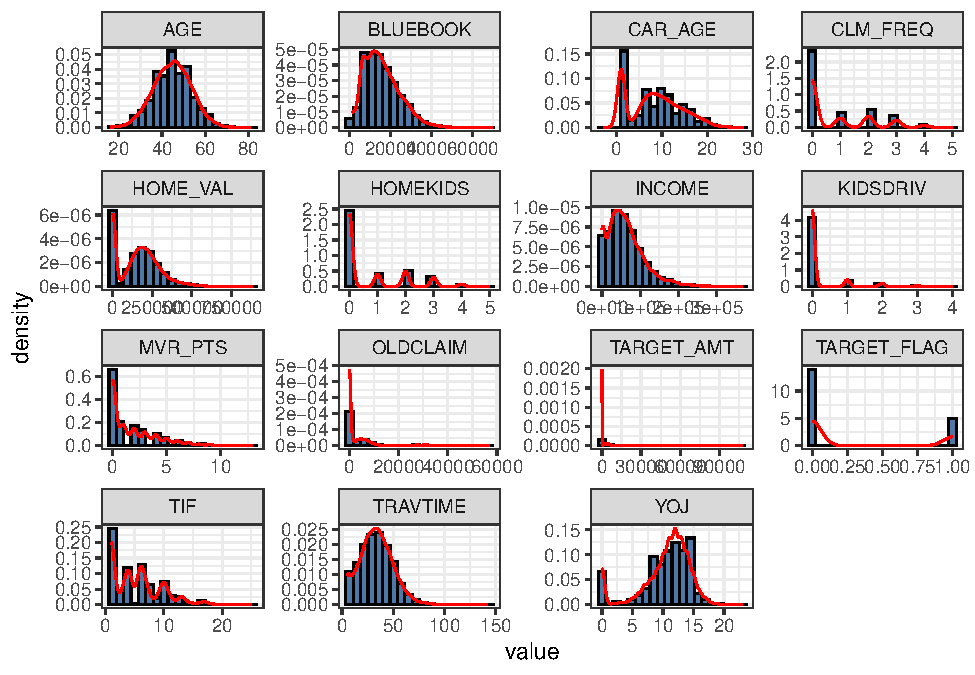
\includegraphics[keepaspectratio]{DATA_621_HW4_Group2_knit_files/figure-latex/density-1.pdf}}

The variable AGE appears to follow a normal distribution. When examining
our first response variable, TARGET\_FLAG, its distribution aligns with
the expected shape of a logit function, ranging between 0 and 1. Several
other variables---such as BLUEBOOK, INCOME, MVR\_PTS, OLDCLAIM,
TARGET\_AMT, TIF, and TRAVTIME---exhibit noticeable right skewness. This
is reasonable, as these values are inherently non-negative and only
restricted on the lower end. Additionally, variables like CAR\_AGE,
HOME\_VAL, and YOJ display bimodal distributions. These patterns suggest
that some transformations may be necessary, and we might also explore
grouping strategies for the bimodal variables.

\textbf{Bar Plots}

Our bar plots show us how our categorical data is divided up.

\pandocbounded{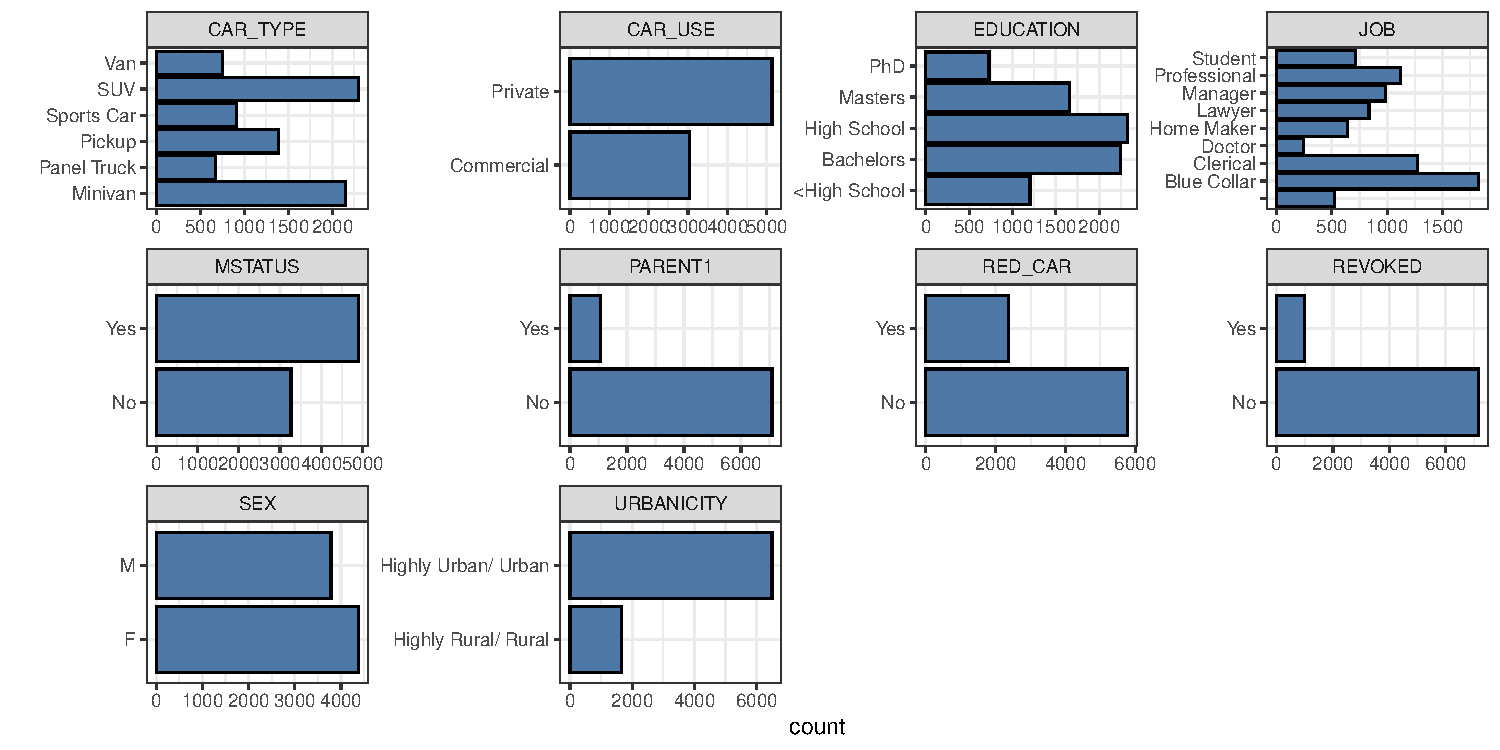
\includegraphics[keepaspectratio]{DATA_621_HW4_Group2_knit_files/figure-latex/bar-1.pdf}}

Additional insights from the data reveal that the majority of vehicles
are either SUVs or Minivans. In terms of education, most drivers have
attained either a High School diploma or a Bachelor's degree. The
dataset also shows that most individuals reside or work in Highly Urban
or Urban environments. Furthermore, vehicle usage is primarily for
personal rather than commercial purposes.

\textbf{Box Plots}

Visualizations can also display the presence of outliers. We expect
quite a few outliers, especially when it comes to the value of cars,
income of drivers, and home values.

\pandocbounded{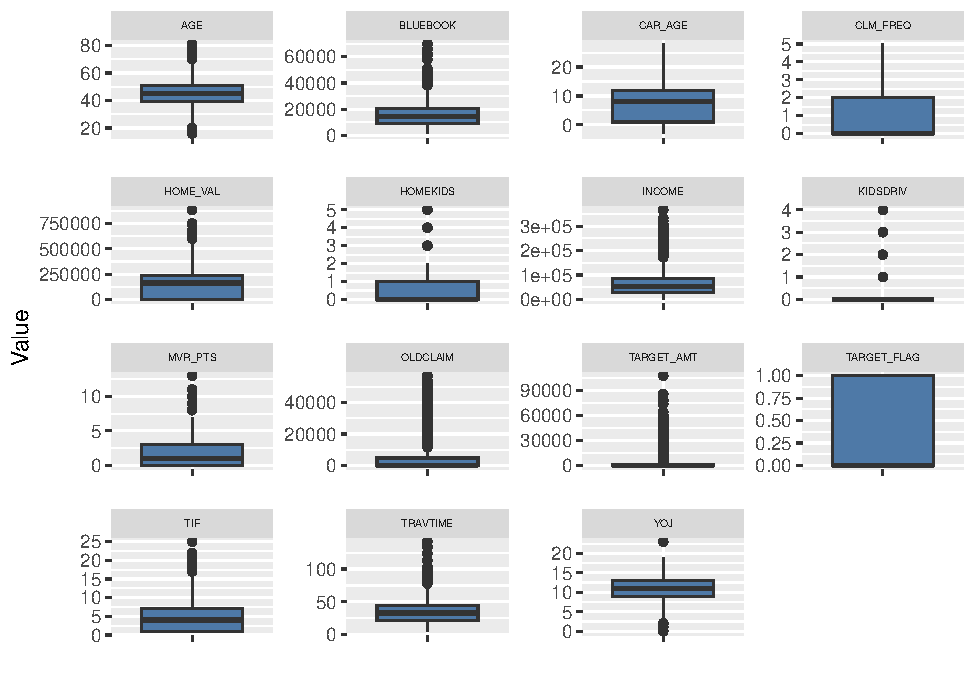
\includegraphics[keepaspectratio]{DATA_621_HW4_Group2_knit_files/figure-latex/boxplot-1.pdf}}

As indicated by the box plots, there are several outliers that need to
be addressed. For instance, BLUEBOOK values show that some insured
vehicles are significantly more expensive than others. Similarly,
HOMEKIDS and KIDSDRIV contain outliers as well---many drivers have no
children, and even fewer have children who drive. Interestingly, the
interquartile range for HOMEKIDS is noticeably higher than that for
KIDSDRIV, which makes sense, as only a portion of the children in a
household are of driving age. Given this relationship, it's reasonable
to expect some correlation between these two variables---an idea we
explore further in the next section.

\textbf{Correlation Matrix}

\pandocbounded{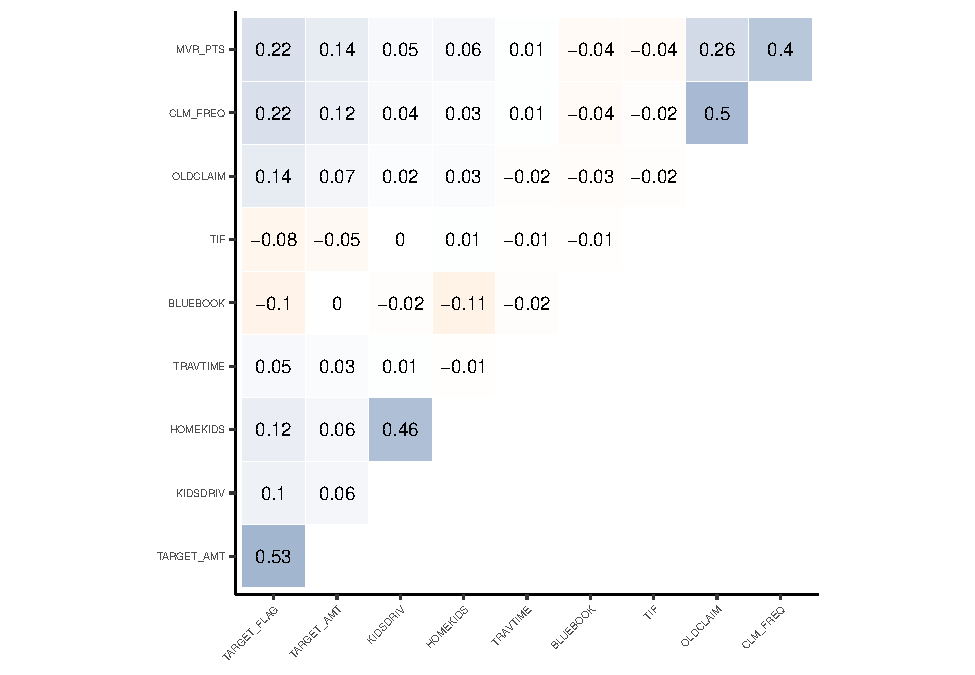
\includegraphics[keepaspectratio]{DATA_621_HW4_Group2_knit_files/figure-latex/corr-plot-1.pdf}}

As expected, we have some moderately strong correlations between some of
our variables. This will have to be addressed with when we build our
models.

\begin{itemize}
\tightlist
\item
  \texttt{KIDSDRIV} and \texttt{HOMEKIDS}: As discussed, we expect
  multicollinearity as if you have children, they may be of age to drive
  already
\item
  \texttt{MVR\_PTS} and \texttt{CLM\_FREQ}: The multicollinearity is
  intuitive as, if you have higher motor vehicle points accumulated from
  negative driving habits, you may be more likely to have accidents and
  require to file more claims than the average driver.
\item
  \texttt{CLM\_FREQ} and \texttt{OLDCLAIM}: There would be some
  multicollinearity since those that file more claims are likely to have
  a higher total claim value over the past 5 years.
\item
  \texttt{TARGET\_AMT} and \texttt{TARGET\_FLAG}: Perhaps most obviously
  of all, since we expect TARGET\_AMT to be zero if the person did not
  crash their car, but greater than zero if they did crash their car.
\end{itemize}

\subsubsection{Missing Values}\label{missing-values}

\begin{table}[H]
\centering\centering
\caption{\label{tab:missing-values}Missing Values Count}
\centering
\begin{tabular}[t]{r|r|r|r|r}
\hline
AGE & YOJ & INCOME & HOME\_VAL & CAR\_AGE\\
\hline
6 & 454 & 445 & 464 & 510\\
\hline
\end{tabular}
\end{table}

We can see we have some columns missing values.

\begin{itemize}
\tightlist
\item
  \texttt{AGE}: This column is only missing a few values and, given that
  it is a normally distributed variable, we have many options to impute
  them
\item
  \texttt{YOJ}: We are missing a lot of values for how many year people
  have been at their job
\item
  \texttt{INCOME}: We don't have how much money they are making in a
  year. It could be that they are not working.
\item
  \texttt{HOME\_VAL}: These missing values may be under the assumption
  they don't own a home and possibly renting. We return to this point in
  a moment.
\item
  \texttt{CAR\_AGE}: The highest amount of values we don't have is how
  old the car is.
\end{itemize}

There is a nuanced point about \texttt{HOME\_VAL}. As aforementioned,
these plausibly represent rentals. However, recall the density plots
earlier; there were many 0s for \texttt{HOME\_VAL}. There cannot
realistically be that many houses actually valued at \$0. It is
possible, then, that the 0s \emph{also} represent rentals. In that case,
we should convert the 0s to missing values, and impute them as we will
the other missing values for this column.

Plotting the \texttt{HOME\_VAL} data without the 0s, we get:

\pandocbounded{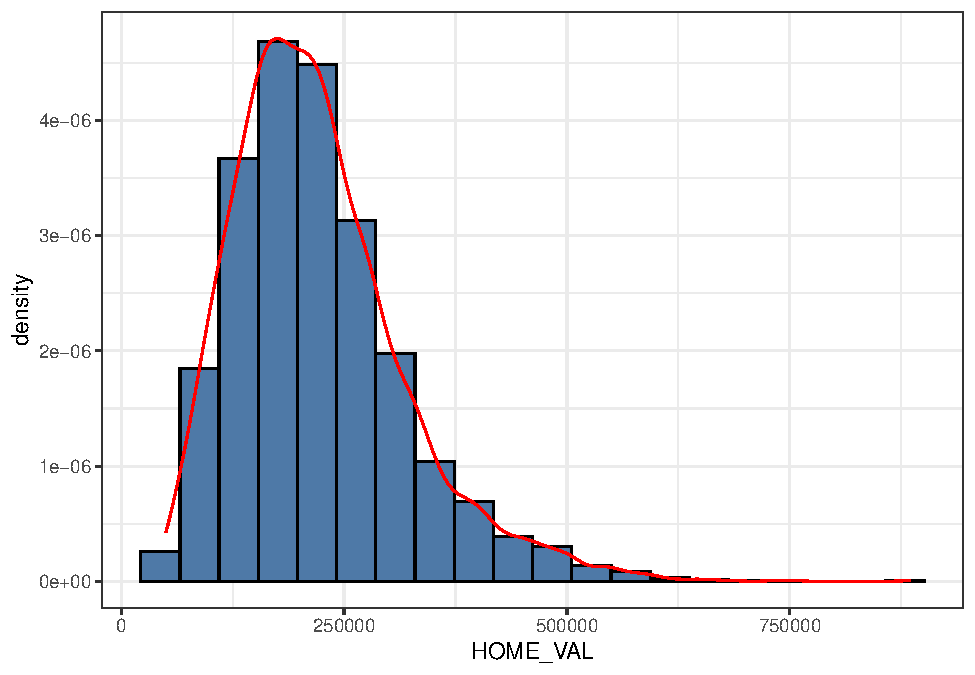
\includegraphics[keepaspectratio]{DATA_621_HW4_Group2_knit_files/figure-latex/unnamed-chunk-2-1.pdf}}

And we can see a much more normal distribution than before.

We now check if there are any other suspect 0s:

\begin{table}[H]
\centering\centering
\caption{\label{tab:Check Zeros}Zero Counts in Training Dataset}
\centering
\begin{tabular}[t]{l|r}
\hline
  & Zero.Count\\
\hline
TARGET\_FLAG & 6008\\
\hline
TARGET\_AMT & 6008\\
\hline
KIDSDRIV & 7180\\
\hline
AGE & 0\\
\hline
HOMEKIDS & 5289\\
\hline
YOJ & 625\\
\hline
INCOME & 615\\
\hline
PARENT1 & 0\\
\hline
HOME\_VAL & 0\\
\hline
MSTATUS & 0\\
\hline
SEX & 0\\
\hline
EDUCATION & 0\\
\hline
JOB & 0\\
\hline
TRAVTIME & 0\\
\hline
CAR\_USE & 0\\
\hline
BLUEBOOK & 0\\
\hline
TIF & 0\\
\hline
CAR\_TYPE & 0\\
\hline
RED\_CAR & 0\\
\hline
OLDCLAIM & 5009\\
\hline
CLM\_FREQ & 5009\\
\hline
REVOKED & 0\\
\hline
MVR\_PTS & 3712\\
\hline
CAR\_AGE & 3\\
\hline
URBANICITY & 0\\
\hline
\end{tabular}
\end{table}

There are no other columns containing suspect 0 values. This concludes
the largely exploratory phase of our analysis; we move now to consider
broader transformations of the data.

\subsection{Data Preparation}\label{data-preparation}

Although we've already carried out some initial data cleaning, this
section focuses on more thorough data transformation to optimize the
performance of both our multiple linear regression and logistic
regression models.

\subsubsection{Missing Values}\label{missing-values-1}

We pick up from the previous section by addressing missing values. As
previously mentioned, the variables with missing data include
\textbf{CAR\_AGE}, \textbf{HOME\_VAL}, \textbf{YOJ}, \textbf{INCOME},
and \textbf{AGE}. It's important to note that we recently increased the
number of missing entries in \textbf{HOME\_VAL} by treating zero values
as \textbf{NAs}. The extent of missing data across these columns is
illustrated below:

\pandocbounded{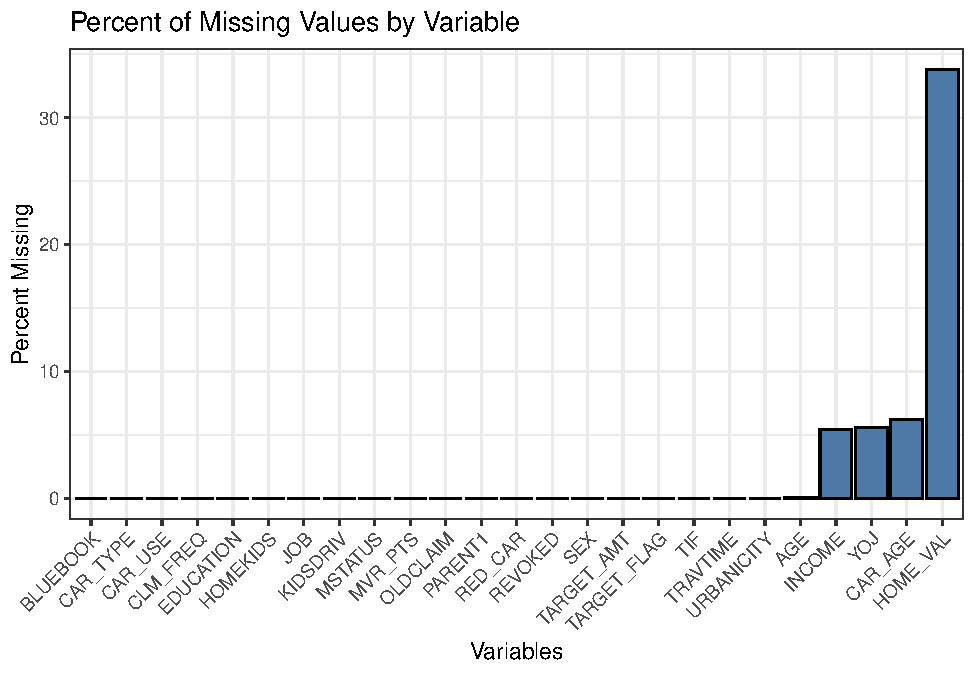
\includegraphics[keepaspectratio]{DATA_621_HW4_Group2_knit_files/figure-latex/percent missing check-1.pdf}}

With the exception of HOME\_VAL, the remaining variables have relatively
few missing values---each with less than 6\% missing. We'll soon move on
to imputing those. However, it's important to take a closer look at
HOME\_VAL again. We've assumed that missing values in this column likely
correspond to renters, which is why we previously replaced zeros with
NAs. Given that the absence of a value here is likely informative, it
would be inappropriate to impute it. Instead, we'll treat HOME\_VAL as a
categorical variable and retain the missing entries as their own
category.

After converting, we can do another bar plot:

\pandocbounded{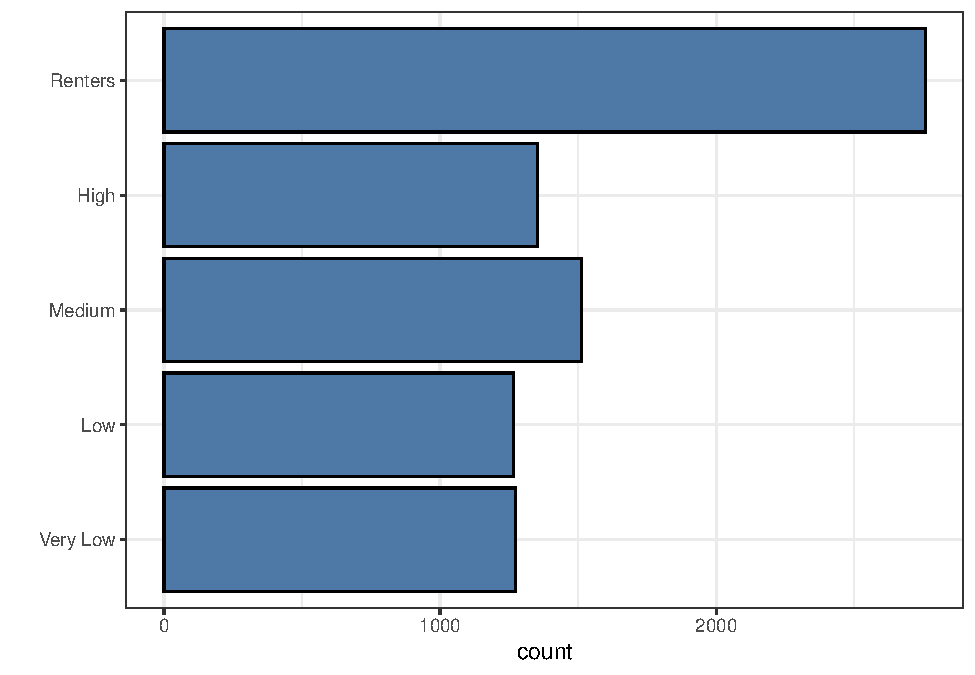
\includegraphics[keepaspectratio]{DATA_621_HW4_Group2_knit_files/figure-latex/unnamed-chunk-3-1.pdf}}

And we see that the data is divided fairly evenly, although ``Missing''
is the largest category.

Let's investigate patterns potentially underlying the missing values:

\begin{Shaded}
\begin{Highlighting}[]
\FunctionTok{plot\_pattern}\NormalTok{(train, }\AttributeTok{square =} \ConstantTok{TRUE}\NormalTok{, }\AttributeTok{rotate =} \ConstantTok{TRUE}\NormalTok{, }\AttributeTok{npat =} \DecValTok{6}\NormalTok{)}
\end{Highlighting}
\end{Shaded}

\pandocbounded{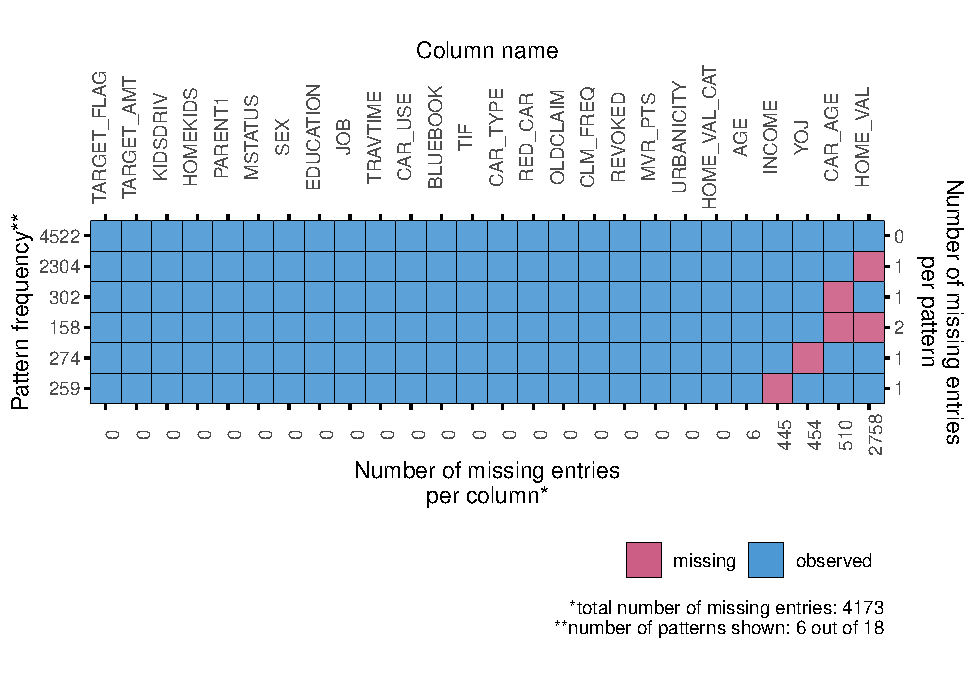
\includegraphics[keepaspectratio]{DATA_621_HW4_Group2_knit_files/figure-latex/missing pattern-1.pdf}}

To begin, we observe that the pattern of missing data is largely
concentrated in \textbf{HOME\_VAL}, which reinforces our earlier
assumption that these missing values likely correspond to renters. This
lends support to the decision to treat HOME\_VAL as a categorical
variable. As a result, we can confidently discard the original
continuous version of HOME\_VAL from our analysis.

Secondly, and on a broader level, the observed missing data patterns
support the use of \textbf{MICE} (Multiple Imputation by Chained
Equations) for handling missing values. Some variables show co-occurring
missingness, indicating possible inter-variable relationships, while
others have missing data in isolation. Given this variability, a uniform
imputation method would be insufficient. MICE is preferred because it
tailors the imputation process to each variable's specific pattern of
missingness.

\subsubsection{Imputations}\label{imputations}

Before we can impute missing values, we perform the train-test split to
avoid data leakage:

We then use MICE to impute. Critically, we ignore the test values when
imputing for both sets, to avoid data leakage.

\begin{verbatim}
## Warning: Number of logged events: 4
## Warning: Number of logged events: 4
\end{verbatim}

\begin{table}[H]
\centering\centering
\caption{\label{tab:summary stats post imputations}Summary Statistics Comparison Across Datasets}
\centering
\begin{tabular}[t]{l|l|l|l}
\hline
Variable\_Stat & Dataset (Pre-Imputations) & Train Imputed & Test Imputed\\
\hline
CAR\_AGE\_min & -3.000000 & -3.000000 & 0.000000\\
\hline
CAR\_AGE\_q1 & 1.000000 & 1.000000 & 1.000000\\
\hline
CAR\_AGE\_median & 8.000000 & 8.000000 & 8.000000\\
\hline
CAR\_AGE\_mean & 8.347639 & 8.365517 & 8.295752\\
\hline
CAR\_AGE\_q3 & 12.000000 & 12.000000 & 12.000000\\
\hline
CAR\_AGE\_max & 27.000000 & 27.000000 & 28.000000\\
\hline
YOJ\_min & 0.000000 & 0.000000 & 0.000000\\
\hline
YOJ\_q1 & 9.000000 & 9.000000 & 9.000000\\
\hline
YOJ\_median & 11.000000 & 11.000000 & 11.000000\\
\hline
YOJ\_mean & 10.499536 & 10.505654 & 10.515441\\
\hline
YOJ\_q3 & 13.000000 & 13.000000 & 13.000000\\
\hline
YOJ\_max & 23.000000 & 23.000000 & 19.000000\\
\hline
INCOME\_min & 0.000000 & 0.000000 & 0.000000\\
\hline
INCOME\_q1 & 28127.500000 & 27907.000000 & 27786.750000\\
\hline
INCOME\_median & 54007.000000 & 53598.000000 & 53841.000000\\
\hline
INCOME\_mean & 62215.300443 & 62089.682514 & 60849.925980\\
\hline
INCOME\_q3 & 85865.500000 & 85752.000000 & 85472.000000\\
\hline
INCOME\_max & 332339.000000 & 332339.000000 & 367030.000000\\
\hline
AGE\_min & 16.000000 & 16.000000 & 17.000000\\
\hline
AGE\_q1 & 39.000000 & 39.000000 & 39.000000\\
\hline
AGE\_median & 45.000000 & 45.000000 & 45.000000\\
\hline
AGE\_mean & 44.781573 & 44.781612 & 44.810733\\
\hline
AGE\_q3 & 51.000000 & 51.000000 & 51.000000\\
\hline
AGE\_max & 81.000000 & 81.000000 & 76.000000\\
\hline
\end{tabular}
\end{table}

The summary statistics are quite promising. For the most part, the
values remain consistent across all three datasets, suggesting that the
distributions in the imputed datasets closely reflect those of the
original. This holds true for both the means and medians. Additionally,
it appears that outliers and edge cases have been managed appropriately.

\subsubsection{Outliers and
Transformations}\label{outliers-and-transformations}

During the data exploration phase, we conducted a preliminary review of
outliers. While the outlier values appeared to be valid, they do
contribute to increased skewness in the data, which can negatively
affect both logistic and linear regression models. To address this, we
applied various data transformations. In evaluating skewness, we
consider values with an absolute skewness above 1 to be \textbf{heavily
skewed}, those between ±0.5 and ±1 to be \textbf{moderately skewed}, and
values between 0 and ±0.5 to be \textbf{lightly skewed}.

We can assess the most appropriate transformations for each variable
using the bestNormalize function.

\begin{table}[H]
\centering\centering
\caption{\label{tab:bestNormalize usage}Best Transformations}
\centering
\begin{tabular}[t]{l|l}
\hline
Variable & Transformation\\
\hline
BLUEBOOK & orderNorm\\
\hline
INCOME & orderNorm\\
\hline
MVR\_PTS & sqrt\_x\\
\hline
OLDCLAIM & center\_scale\\
\hline
TIF & yeojohnson\\
\hline
TRAVTIME & boxcox\\
\hline
YOJ & sqrt\_x\\
\hline
CLM\_FREQ & sqrt\_x\\
\hline
CAR\_AGE & yeojohnson\\
\hline
\end{tabular}
\end{table}

Once again, it's crucial to avoid data leakage by ensuring that all
transformation parameters are derived solely from the training set.
These same parameters should then be applied consistently to the
evaluation and test sets.

\begin{verbatim}
## Warning: There was 1 warning in `summarise()`.
## i In argument: `across(...)`.
## Caused by warning:
## ! The `...` argument of `across()` is deprecated as of dplyr 1.1.0.
## Supply arguments directly to `.fns` through an anonymous function instead.
## 
##   # Previously
##   across(a:b, mean, na.rm = TRUE)
## 
##   # Now
##   across(a:b, \(x) mean(x, na.rm = TRUE))
\end{verbatim}

\begin{table}[H]
\centering\centering
\caption{\label{tab:skew before and after}Pre and Post Transformation Skewness Comparison}
\centering
\begin{tabular}[t]{l|r|r}
\hline
Variable & Pre-Transformation Skew & Post-Transformation Skew\\
\hline
BLUEBOOK & 0.791 & 0.042\\
\hline
INCOME & 1.195 & 0.146\\
\hline
MVR\_PTS & 1.337 & 0.393\\
\hline
OLDCLAIM & 3.190 & 3.190\\
\hline
TIF & 0.890 & -0.034\\
\hline
TRAVTIME & 0.471 & -0.043\\
\hline
YOJ & -1.208 & -2.253\\
\hline
CLM\_FREQ & 1.217 & 0.711\\
\hline
CAR\_AGE & 0.268 & -0.188\\
\hline
\end{tabular}
\end{table}

In general, the applied transformations successfully reduced skewness to
more acceptable levels across most variables. However, OLDCLAIM---the
most skewed variable---showed little to no improvement. Despite this,
the overall distribution of the dataset is now significantly closer to
normality, which should enhance the performance of our models moving
forward.

\subsubsection{Outliers}\label{outliers}

Despite applying transformations, some outliers still remain. To address
this, we will use outlier replacement techniques. As before, it's
essential to calculate the replacement thresholds based solely on the
training set and apply them consistently across all datasets. This
approach ensures we prevent any risk of data leakage.

\subsubsection{Encoding,
Center/Scale/NearZeroVariance}\label{encoding-centerscalenearzerovariance}

The last step in our data preparation process involves encoding
categorical variables using one-hot encoding (OHC). Additionally, we
center and scale (CS) all continuous variables to prevent extreme values
from skewing the model---using statistics derived solely from the
training data to avoid data leakage. We also check continuous variables
for near-zero variance (NZV), as such features provide little predictive
power. For ordinal variables, we treat them as continuous since the
spacing between values is both consistent and meaningful. Both
centering/scaling and NZV filtering can be streamlined through a single
step in a preprocessing pipeline.

The dataframes are now fully processed. We are ready to move on to the
modeling phase.

\subsection{Modeling}\label{modeling}

With preprocessing complete, we're now ready to begin modeling. In the
first phase, we'll develop \textbf{logistic regression models} to
predict the likelihood of a person being involved in a car accident. In
the second phase, we'll construct \textbf{multiple linear regression
models} to estimate the payout amount in cases where a crash has
occurred.

\subsubsection{Logistic regression}\label{logistic-regression}

As a reminder, our initial objective is to predict whether a driver was
involved in a crash. Since our dataset includes both original and
transformed versions of some variables, it's important to ensure we
don't include duplicate information in the model. To maintain clarity
and prevent redundancy, we will explicitly categorize the variables
being used.

\begin{table}[H]
\centering\centering
\caption{\label{tab:unnamed-chunk-8}Variables Summary}
\centering
\begin{tabular}[t]{l|l}
\hline
Category & Variables\\
\hline
Encoded & SEX.F, SEX.M, EDUCATION.L, EDUCATION.Q, EDUCATION.C, JOBBlue Collar, JOBClerical, JOBDoctor, JOBHome Maker, JOBLawyer, JOBManager, JOBProfessional, JOBStudent, CAR\_USECommercial, CAR\_USEPrivate, CAR\_TYPEMinivan, CAR\_TYPEPanel Truck, CAR\_TYPEPickup, CAR\_TYPESports Car, CAR\_TYPESUV, CAR\_TYPEVan, URBANICITYHighly Rural/ Rural, URBANICITYHighly Urban/ Urban, HOME\_VAL\_CAT.Very Low, HOME\_VAL\_CAT.Low, HOME\_VAL\_CAT.Medium, HOME\_VAL\_CAT.High, HOME\_VAL\_CAT.Missing, RED\_CAR.No, RED\_CAR.Yes, REVOKED.No, REVOKED.Yes, PARENT1.No, PARENT1.Yes, MSTATUS.No, MSTATUS.Yes\\
\hline
Original & KIDSDRIV, AGE, HOMEKIDS, YOJ, INCOME, PARENT1, MSTATUS, SEX, EDUCATION, JOB, TRAVTIME, CAR\_USE, BLUEBOOK, TIF, CAR\_TYPE, RED\_CAR, OLDCLAIM, CLM\_FREQ, REVOKED, MVR\_PTS, CAR\_AGE, URBANICITY, HOME\_VAL\_CAT\\
\hline
Transformed & BLUEBOOK\_transformed, INCOME\_transformed, MVR\_PTS\_transformed, OLDCLAIM\_transformed, TIF\_transformed, TRAVTIME\_transformed, YOJ\_transformed, CLM\_FREQ\_transformed, CAR\_AGE\_transformed\\
\hline
\end{tabular}
\end{table}

We must also proceed with caution due to the \textbf{One-Hot Encoding
(OHC)} applied to our categorical variables. This encoding can introduce
\textbf{multicollinearity}, especially among the resulting dummy
variables. For binary categorical variables, we can safely drop one of
the two encoded columns, as the remaining one still captures all
necessary information. However, for variables with more than two
categories, multicollinearity becomes more complex and may require more
advanced handling strategies---which we'll address shortly.

\paragraph{Model 1}\label{model-1}

To begin, we'll construct a straightforward model to establish a
baseline understanding of our data. We'll focus on using the
\textbf{transformed variables}, as they are all continuous and generally
more manageable. Additionally, we expect these transformed features to
outperform their original versions in terms of model effectiveness.

\begin{Shaded}
\begin{Highlighting}[]
\NormalTok{simple\_model1 }\OtherTok{\textless{}{-}} \FunctionTok{glm}\NormalTok{(TARGET\_FLAG }\SpecialCharTok{\textasciitilde{}}\NormalTok{ ., }\AttributeTok{data =}\NormalTok{ train\_final[, }\FunctionTok{c}\NormalTok{(transformed\_columns, encoded\_columns, }\StringTok{"TARGET\_FLAG"}\NormalTok{)], }\AttributeTok{family =} \StringTok{"binomial"}\NormalTok{)}
\FunctionTok{summary}\NormalTok{(simple\_model1)}
\end{Highlighting}
\end{Shaded}

\begin{verbatim}
## 
## Call:
## glm(formula = TARGET_FLAG ~ ., family = "binomial", data = train_final[, 
##     c(transformed_columns, encoded_columns, "TARGET_FLAG")])
## 
## Coefficients: (9 not defined because of singularities)
##                                 Estimate Std. Error z value Pr(>|z|)    
## (Intercept)                      0.05574    0.13818   0.403  0.68666    
## BLUEBOOK_transformed            -0.21664    0.02212  -9.793  < 2e-16 ***
## INCOME_transformed              -0.22395    0.03350  -6.684 2.32e-11 ***
## MVR_PTS_transformed              0.24224    0.01780  13.608  < 2e-16 ***
## OLDCLAIM_transformed            -0.11981    0.01905  -6.288 3.21e-10 ***
## TIF_transformed                 -0.23220    0.01574 -14.755  < 2e-16 ***
## TRAVTIME_transformed             0.26369    0.01626  16.219  < 2e-16 ***
## YOJ_transformed                 -0.08354    0.01940  -4.306 1.67e-05 ***
## CLM_FREQ_transformed             0.36401    0.02708  13.443  < 2e-16 ***
## CAR_AGE_transformed             -0.06006    0.02170  -2.767  0.00565 ** 
## SEX.F                            0.03524    0.05865   0.601  0.54796    
## SEX.M                                 NA         NA      NA       NA    
## EDUCATION.L                     -0.20571    0.08609  -2.390  0.01687 *  
## EDUCATION.Q                      0.27093    0.04915   5.512 3.55e-08 ***
## EDUCATION.C                      0.14289    0.04169   3.427  0.00061 ***
## `JOBBlue Collar`                 0.48525    0.09379   5.174 2.29e-07 ***
## JOBClerical                      0.55794    0.10098   5.525 3.29e-08 ***
## JOBDoctor                       -0.18215    0.13389  -1.361  0.17367    
## `JOBHome Maker`                  0.27626    0.11381   2.427  0.01521 *  
## JOBLawyer                        0.40011    0.09066   4.413 1.02e-05 ***
## JOBManager                      -0.35423    0.08924  -3.970 7.20e-05 ***
## JOBProfessional                  0.29441    0.09082   3.242  0.00119 ** 
## JOBStudent                       0.06058    0.11568   0.524  0.60051    
## CAR_USECommercial                0.80164    0.04921  16.289  < 2e-16 ***
## CAR_USEPrivate                        NA         NA      NA       NA    
## CAR_TYPEMinivan                 -0.66597    0.06764  -9.846  < 2e-16 ***
## `CAR_TYPEPanel Truck`           -0.09080    0.07718  -1.176  0.23943    
## CAR_TYPEPickup                  -0.14177    0.06721  -2.109  0.03492 *  
## `CAR_TYPESports Car`             0.23356    0.09199   2.539  0.01111 *  
## CAR_TYPESUV                      0.05328    0.08380   0.636  0.52493    
## CAR_TYPEVan                           NA         NA      NA       NA    
## `URBANICITYHighly Rural/ Rural` -2.48282    0.06146 -40.399  < 2e-16 ***
## `URBANICITYHighly Urban/ Urban`       NA         NA      NA       NA    
## `HOME_VAL_CAT.Very Low`         -0.39760    0.05783  -6.875 6.18e-12 ***
## HOME_VAL_CAT.Low                -0.37895    0.05656  -6.700 2.08e-11 ***
## HOME_VAL_CAT.Medium             -0.35455    0.05319  -6.665 2.64e-11 ***
## HOME_VAL_CAT.High               -0.38809    0.06561  -5.915 3.32e-09 ***
## HOME_VAL_CAT.Missing                  NA         NA      NA       NA    
## RED_CAR.No                      -0.01745    0.04639  -0.376  0.70686    
## RED_CAR.Yes                           NA         NA      NA       NA    
## REVOKED.No                      -0.88408    0.04934 -17.918  < 2e-16 ***
## REVOKED.Yes                           NA         NA      NA       NA    
## PARENT1.No                      -0.71558    0.04898 -14.610  < 2e-16 ***
## PARENT1.Yes                           NA         NA      NA       NA    
## MSTATUS.No                       0.35077    0.04281   8.193 2.54e-16 ***
## MSTATUS.Yes                           NA         NA      NA       NA    
## ---
## Signif. codes:  0 '***' 0.001 '**' 0.01 '*' 0.05 '.' 0.1 ' ' 1
## 
## (Dispersion parameter for binomial family taken to be 1)
## 
##     Null deviance: 33055  on 28564  degrees of freedom
## Residual deviance: 25417  on 28528  degrees of freedom
## AIC: 25491
## 
## Number of Fisher Scoring iterations: 5
\end{verbatim}

Given the results, we'll proceed by eliminating variables that
contribute to multicollinearity. For binary variables, we can remove
either one of the two encoded columns, as they carry equivalent
information. For variables with more than two categories, we'll drop the
one that shows the weakest correlation with the target variable, under
the assumption that it will have the least influence on the model's
performance.

\begin{table}[H]
\centering\centering
\caption{\label{tab:cor matrix to remove columns}Correlations with TARGET FLAG}
\centering
\begin{tabular}[t]{l|r}
\hline
  & x\\
\hline
SEX.F & 0.0318414\\
\hline
SEX.M & -0.0318414\\
\hline
EDUCATION.L & -0.1316931\\
\hline
EDUCATION.Q & 0.0172592\\
\hline
EDUCATION.C & 0.0841712\\
\hline
JOBBlue Collar & 0.1043799\\
\hline
JOBClerical & 0.0261655\\
\hline
JOBDoctor & -0.0530153\\
\hline
JOBHome Maker & 0.0123769\\
\hline
JOBLawyer & -0.0629416\\
\hline
JOBManager & -0.1006736\\
\hline
JOBProfessional & -0.0337543\\
\hline
JOBStudent & 0.0734056\\
\hline
CAR\_USECommercial & 0.1427534\\
\hline
CAR\_USEPrivate & -0.1427534\\
\hline
CAR\_TYPEMinivan & -0.1339852\\
\hline
CAR\_TYPEPanel Truck & -0.0020186\\
\hline
CAR\_TYPEPickup & 0.0481774\\
\hline
CAR\_TYPESports Car & 0.0574468\\
\hline
CAR\_TYPESUV & 0.0515462\\
\hline
CAR\_TYPEVan & 0.0018546\\
\hline
URBANICITYHighly Rural/ Rural & -0.2342684\\
\hline
URBANICITYHighly Urban/ Urban & 0.2342684\\
\hline
HOME\_VAL\_CAT.Very Low & 0.0047065\\
\hline
HOME\_VAL\_CAT.Low & -0.0167182\\
\hline
HOME\_VAL\_CAT.Medium & -0.0648757\\
\hline
HOME\_VAL\_CAT.High & -0.1241068\\
\hline
HOME\_VAL\_CAT.Missing & 0.1585339\\
\hline
RED\_CAR.No & 0.0093489\\
\hline
RED\_CAR.Yes & -0.0093489\\
\hline
REVOKED.No & -0.1433965\\
\hline
REVOKED.Yes & 0.1433965\\
\hline
PARENT1.No & -0.1697927\\
\hline
PARENT1.Yes & 0.1697927\\
\hline
MSTATUS.No & 0.1473048\\
\hline
MSTATUS.Yes & -0.1473048\\
\hline
TARGET\_FLAG & 1.0000000\\
\hline
\end{tabular}
\end{table}

Again, with the binary columns, we can just remove any one them. Thus,
we'll remove:

\begin{itemize}
\tightlist
\item
  SEX.M
\item
  CAR\_USEPrivate
\item
  \texttt{URBANICITYHighly\ Urban/\ Urban}
\item
  RED\_CAR.Yes
\item
  REVOKED.Yes
\item
  PARENT1.Yes
\item
  MSTATUS.Yes
\end{itemize}

Of the categorical, but not binary, variables we will remove the least
informative:

\begin{itemize}
\tightlist
\item
  EDUCATION.Q
\item
  JOBHome Maker
\item
  CAR\_TYPEVan
\item
  HOME\_VAL\_CAT.Low
\end{itemize}

We now rerun the simple model without these columns to get a look at
some of the coefficients.

\begin{Shaded}
\begin{Highlighting}[]
\NormalTok{simple\_model2 }\OtherTok{\textless{}{-}} \FunctionTok{glm}\NormalTok{(TARGET\_FLAG }\SpecialCharTok{\textasciitilde{}}\NormalTok{ ., }\AttributeTok{data =}\NormalTok{ train\_final[, }\FunctionTok{c}\NormalTok{(transformed\_columns, encoded\_columns\_filtered, }\StringTok{"TARGET\_FLAG"}\NormalTok{)], }\AttributeTok{family =} \StringTok{"binomial"}\NormalTok{)}
\FunctionTok{summary}\NormalTok{(simple\_model2)}
\end{Highlighting}
\end{Shaded}

\begin{verbatim}
## 
## Call:
## glm(formula = TARGET_FLAG ~ ., family = "binomial", data = train_final[, 
##     c(transformed_columns, encoded_columns_filtered, "TARGET_FLAG")])
## 
## Coefficients:
##                                 Estimate Std. Error z value Pr(>|z|)    
## (Intercept)                     -0.14454    0.12461  -1.160  0.24609    
## BLUEBOOK_transformed            -0.21551    0.02211  -9.745  < 2e-16 ***
## INCOME_transformed              -0.22659    0.03194  -7.094 1.30e-12 ***
## MVR_PTS_transformed              0.24349    0.01779  13.685  < 2e-16 ***
## OLDCLAIM_transformed            -0.12331    0.01903  -6.480 9.16e-11 ***
## TIF_transformed                 -0.23204    0.01571 -14.766  < 2e-16 ***
## TRAVTIME_transformed             0.26208    0.01625  16.129  < 2e-16 ***
## YOJ_transformed                 -0.09174    0.01909  -4.806 1.54e-06 ***
## CLM_FREQ_transformed             0.36370    0.02707  13.438  < 2e-16 ***
## CAR_AGE_transformed             -0.06561    0.02163  -3.034  0.00242 ** 
## SEX.F                            0.04996    0.05844   0.855  0.39260    
## EDUCATION.L                     -0.36568    0.08224  -4.446 8.73e-06 ***
## EDUCATION.C                      0.10844    0.04026   2.693  0.00707 ** 
## `JOBBlue Collar`                 0.28450    0.07093   4.011 6.05e-05 ***
## JOBClerical                      0.33886    0.07042   4.812 1.50e-06 ***
## JOBDoctor                       -0.07637    0.12329  -0.619  0.53565    
## JOBLawyer                        0.23378    0.07558   3.093  0.00198 ** 
## JOBManager                      -0.55033    0.07095  -7.757 8.72e-15 ***
## JOBProfessional                  0.04378    0.06672   0.656  0.51174    
## JOBStudent                      -0.16478    0.08038  -2.050  0.04036 *  
## CAR_USECommercial                0.74458    0.04784  15.563  < 2e-16 ***
## CAR_TYPEMinivan                 -0.68327    0.06746 -10.128  < 2e-16 ***
## `CAR_TYPEPanel Truck`           -0.07561    0.07698  -0.982  0.32603    
## CAR_TYPEPickup                  -0.14146    0.06716  -2.106  0.03519 *  
## `CAR_TYPESports Car`             0.20999    0.09178   2.288  0.02215 *  
## CAR_TYPESUV                      0.02517    0.08356   0.301  0.76326    
## `URBANICITYHighly Rural/ Rural` -2.47380    0.06135 -40.321  < 2e-16 ***
## `HOME_VAL_CAT.Very Low`          0.02691    0.05947   0.453  0.65084    
## HOME_VAL_CAT.Medium              0.01552    0.05772   0.269  0.78799    
## HOME_VAL_CAT.High                0.01103    0.07376   0.150  0.88109    
## HOME_VAL_CAT.Missing             0.39769    0.05633   7.060 1.67e-12 ***
## RED_CAR.No                      -0.01573    0.04631  -0.340  0.73411    
## REVOKED.No                      -0.88511    0.04926 -17.967  < 2e-16 ***
## PARENT1.No                      -0.71243    0.04892 -14.563  < 2e-16 ***
## MSTATUS.No                       0.34353    0.04276   8.035 9.38e-16 ***
## ---
## Signif. codes:  0 '***' 0.001 '**' 0.01 '*' 0.05 '.' 0.1 ' ' 1
## 
## (Dispersion parameter for binomial family taken to be 1)
## 
##     Null deviance: 33055  on 28564  degrees of freedom
## Residual deviance: 25449  on 28530  degrees of freedom
## AIC: 25519
## 
## Number of Fisher Scoring iterations: 5
\end{verbatim}

At this point, we've eliminated all singularities from the model.
However, since the \textbf{Deviance} and \textbf{AIC} remain unchanged,
it's clear that the model itself hasn't improved---only the
\textbf{stability and interpretability} of the coefficients has, thanks
to the removal of perfect multicollinearity. That said, several
variables remain statistically insignificant and may be detracting from
model performance. Additionally, although perfect multicollinearity has
been addressed, some degree of \textbf{collinearity} still exists,
particularly among the categorical predictors. To further refine the
model, we'll use a combination of the \textbf{\texttt{vif()} function}
and the previously generated \textbf{correlation matrix}.

\begin{table}[H]
\centering\centering
\caption{\label{tab:VIF simple_model 2}VIF Values simple model 2}
\centering
\begin{tabular}[t]{l|r}
\hline
  & x\\
\hline
BLUEBOOK\_transformed & 1.996188\\
\hline
INCOME\_transformed & 3.785523\\
\hline
MVR\_PTS\_transformed & 1.194844\\
\hline
OLDCLAIM\_transformed & 1.772831\\
\hline
TIF\_transformed & 1.011940\\
\hline
TRAVTIME\_transformed & 1.037135\\
\hline
YOJ\_transformed & 1.646669\\
\hline
CLM\_FREQ\_transformed & 1.668053\\
\hline
CAR\_AGE\_transformed & 1.931736\\
\hline
SEX.F & 3.509678\\
\hline
EDUCATION.L & 3.768989\\
\hline
EDUCATION.C & 1.457579\\
\hline
`JOBBlue Collar` & 3.971995\\
\hline
JOBClerical & 2.765126\\
\hline
JOBDoctor & 1.379093\\
\hline
JOBLawyer & 1.993747\\
\hline
JOBManager & 1.699790\\
\hline
JOBProfessional & 2.082224\\
\hline
JOBStudent & 2.422258\\
\hline
CAR\_USECommercial & 2.319272\\
\hline
CAR\_TYPEMinivan & 3.058352\\
\hline
`CAR\_TYPEPanel Truck` & 1.974441\\
\hline
CAR\_TYPEPickup & 2.854481\\
\hline
`CAR\_TYPESports Car` & 3.725190\\
\hline
CAR\_TYPESUV & 6.081278\\
\hline
`URBANICITYHighly Rural/ Rural` & 1.133181\\
\hline
`HOME\_VAL\_CAT.Very Low` & 1.959488\\
\hline
HOME\_VAL\_CAT.Medium & 1.984954\\
\hline
HOME\_VAL\_CAT.High & 2.342268\\
\hline
HOME\_VAL\_CAT.Missing & 3.149562\\
\hline
RED\_CAR.No & 1.832713\\
\hline
REVOKED.No & 1.328290\\
\hline
PARENT1.No & 1.367305\\
\hline
MSTATUS.No & 1.878037\\
\hline
\end{tabular}
\end{table}

Given this information, we opt to remove CAR\_TYPESUV which has a VIF
value of over 6. We will then fit a new model.

\begin{Shaded}
\begin{Highlighting}[]
\NormalTok{encoded\_columns\_filtered2 }\OtherTok{\textless{}{-}} \FunctionTok{setdiff}\NormalTok{(encoded\_columns\_filtered, }\StringTok{"CAR\_TYPESUV"}\NormalTok{)}

\NormalTok{transformed\_model }\OtherTok{\textless{}{-}} \FunctionTok{glm}\NormalTok{(TARGET\_FLAG }\SpecialCharTok{\textasciitilde{}}\NormalTok{ ., }\AttributeTok{data =}\NormalTok{ train\_final[, }\FunctionTok{c}\NormalTok{(transformed\_columns, encoded\_columns\_filtered2, }\StringTok{"TARGET\_FLAG"}\NormalTok{)], }\AttributeTok{family =} \StringTok{"binomial"}\NormalTok{)}

\FunctionTok{summary}\NormalTok{(transformed\_model)}
\end{Highlighting}
\end{Shaded}

\begin{verbatim}
## 
## Call:
## glm(formula = TARGET_FLAG ~ ., family = "binomial", data = train_final[, 
##     c(transformed_columns, encoded_columns_filtered2, "TARGET_FLAG")])
## 
## Coefficients:
##                                 Estimate Std. Error z value Pr(>|z|)    
## (Intercept)                     -0.13486    0.12038  -1.120 0.262606    
## BLUEBOOK_transformed            -0.21846    0.01983 -11.016  < 2e-16 ***
## INCOME_transformed              -0.22707    0.03190  -7.118 1.09e-12 ***
## MVR_PTS_transformed              0.24338    0.01779  13.682  < 2e-16 ***
## OLDCLAIM_transformed            -0.12339    0.01903  -6.485 8.85e-11 ***
## TIF_transformed                 -0.23197    0.01571 -14.763  < 2e-16 ***
## TRAVTIME_transformed             0.26220    0.01624  16.141  < 2e-16 ***
## YOJ_transformed                 -0.09158    0.01908  -4.800 1.59e-06 ***
## CLM_FREQ_transformed             0.36389    0.02706  13.449  < 2e-16 ***
## CAR_AGE_transformed             -0.06551    0.02163  -3.029 0.002452 ** 
## SEX.F                            0.05975    0.04855   1.231 0.218432    
## EDUCATION.L                     -0.36447    0.08214  -4.437 9.11e-06 ***
## EDUCATION.C                      0.10905    0.04021   2.712 0.006683 ** 
## `JOBBlue Collar`                 0.28776    0.07010   4.105 4.04e-05 ***
## JOBClerical                      0.34011    0.07030   4.838 1.31e-06 ***
## JOBDoctor                       -0.07424    0.12309  -0.603 0.546425    
## JOBLawyer                        0.23564    0.07533   3.128 0.001758 ** 
## JOBManager                      -0.54900    0.07081  -7.753 8.99e-15 ***
## JOBProfessional                  0.04506    0.06658   0.677 0.498533    
## JOBStudent                      -0.16294    0.08014  -2.033 0.042038 *  
## CAR_USECommercial                0.74176    0.04691  15.812  < 2e-16 ***
## CAR_TYPEMinivan                 -0.69796    0.04657 -14.988  < 2e-16 ***
## `CAR_TYPEPanel Truck`           -0.08034    0.07533  -1.066 0.286207    
## CAR_TYPEPickup                  -0.15544    0.04853  -3.203 0.001359 ** 
## `CAR_TYPESports Car`             0.18730    0.05244   3.572 0.000355 ***
## `URBANICITYHighly Rural/ Rural` -2.47381    0.06136 -40.320  < 2e-16 ***
## `HOME_VAL_CAT.Very Low`          0.02674    0.05946   0.450 0.652928    
## HOME_VAL_CAT.Medium              0.01535    0.05772   0.266 0.790247    
## HOME_VAL_CAT.High                0.01053    0.07375   0.143 0.886487    
## HOME_VAL_CAT.Missing             0.39714    0.05630   7.054 1.74e-12 ***
## RED_CAR.No                      -0.01522    0.04629  -0.329 0.742239    
## REVOKED.No                      -0.88532    0.04926 -17.973  < 2e-16 ***
## PARENT1.No                      -0.71215    0.04891 -14.561  < 2e-16 ***
## MSTATUS.No                       0.34373    0.04275   8.041 8.94e-16 ***
## ---
## Signif. codes:  0 '***' 0.001 '**' 0.01 '*' 0.05 '.' 0.1 ' ' 1
## 
## (Dispersion parameter for binomial family taken to be 1)
## 
##     Null deviance: 33055  on 28564  degrees of freedom
## Residual deviance: 25449  on 28531  degrees of freedom
## AIC: 25517
## 
## Number of Fisher Scoring iterations: 5
\end{verbatim}

Now let's remove SEX and RED\_CAR, both of which are not significant
predictors.

\begin{verbatim}
## 
## Call:
## glm(formula = TARGET_FLAG ~ ., family = "binomial", data = train_final[, 
##     c(transformed_columns, encoded_columns_filtered3, "TARGET_FLAG")])
## 
## Coefficients:
##                                 Estimate Std. Error z value Pr(>|z|)    
## (Intercept)                     -0.09091    0.11204  -0.811 0.417150    
## BLUEBOOK_transformed            -0.21442    0.01955 -10.965  < 2e-16 ***
## INCOME_transformed              -0.22798    0.03189  -7.149 8.73e-13 ***
## MVR_PTS_transformed              0.24358    0.01778  13.696  < 2e-16 ***
## OLDCLAIM_transformed            -0.12355    0.01902  -6.495 8.31e-11 ***
## TIF_transformed                 -0.23195    0.01571 -14.767  < 2e-16 ***
## TRAVTIME_transformed             0.26232    0.01624  16.150  < 2e-16 ***
## YOJ_transformed                 -0.09194    0.01908  -4.820 1.44e-06 ***
## CLM_FREQ_transformed             0.36392    0.02706  13.450  < 2e-16 ***
## CAR_AGE_transformed             -0.06465    0.02162  -2.991 0.002781 ** 
## EDUCATION.L                     -0.36410    0.08214  -4.433 9.31e-06 ***
## EDUCATION.C                      0.11331    0.04006   2.828 0.004683 ** 
## `JOBBlue Collar`                 0.28869    0.07008   4.120 3.80e-05 ***
## JOBClerical                      0.33431    0.07015   4.766 1.88e-06 ***
## JOBDoctor                       -0.08245    0.12286  -0.671 0.502173    
## JOBLawyer                        0.23140    0.07523   3.076 0.002099 ** 
## JOBManager                      -0.55354    0.07061  -7.840 4.52e-15 ***
## JOBProfessional                  0.03995    0.06643   0.601 0.547566    
## JOBStudent                      -0.16463    0.08006  -2.056 0.039756 *  
## CAR_USECommercial                0.73046    0.04600  15.879  < 2e-16 ***
## CAR_TYPEMinivan                 -0.72056    0.04293 -16.785  < 2e-16 ***
## `CAR_TYPEPanel Truck`           -0.11359    0.07050  -1.611 0.107166    
## CAR_TYPEPickup                  -0.17425    0.04605  -3.784 0.000155 ***
## `CAR_TYPESports Car`             0.19852    0.05170   3.840 0.000123 ***
## `URBANICITYHighly Rural/ Rural` -2.47207    0.06133 -40.309  < 2e-16 ***
## `HOME_VAL_CAT.Very Low`          0.02883    0.05942   0.485 0.627578    
## HOME_VAL_CAT.Medium              0.01525    0.05768   0.264 0.791497    
## HOME_VAL_CAT.High                0.00832    0.07372   0.113 0.910138    
## HOME_VAL_CAT.Missing             0.39809    0.05628   7.074 1.51e-12 ***
## REVOKED.No                      -0.88599    0.04925 -17.989  < 2e-16 ***
## PARENT1.No                      -0.71671    0.04877 -14.696  < 2e-16 ***
## MSTATUS.No                       0.34244    0.04272   8.016 1.09e-15 ***
## ---
## Signif. codes:  0 '***' 0.001 '**' 0.01 '*' 0.05 '.' 0.1 ' ' 1
## 
## (Dispersion parameter for binomial family taken to be 1)
## 
##     Null deviance: 33055  on 28564  degrees of freedom
## Residual deviance: 25450  on 28533  degrees of freedom
## AIC: 25514
## 
## Number of Fisher Scoring iterations: 5
\end{verbatim}

At this stage, all predictors in our model are statistically
significant, and collinearity is minimal. However, because this model
was built using transformed variables, interpretation becomes more
complex, and applying it to new data requires replicating the exact same
transformation steps. This limitation leads us to the development of our
next model.

\paragraph{Model 2}\label{model-2}

Now that we have found the predictors we would like to include in our
model, we can try using the non-transformed versions of the variables
and recreating the model.

\begin{verbatim}
## 
## Call:
## glm(formula = TARGET_FLAG ~ ., family = "binomial", data = train_final[, 
##     c(original_non_cat, encoded_columns_filtered3, "TARGET_FLAG")])
## 
## Coefficients:
##                                  Estimate Std. Error z value Pr(>|z|)    
## (Intercept)                     -0.205525   0.098698  -2.082 0.037310 *  
## KIDSDRIV                         0.234527   0.017074  13.736  < 2e-16 ***
## AGE                             -0.064419   0.018835  -3.420 0.000626 ***
## HOMEKIDS                        -0.001323   0.023109  -0.057 0.954338    
## YOJ                              0.036972   0.017055   2.168 0.030168 *  
## INCOME                          -0.232389   0.026699  -8.704  < 2e-16 ***
## TRAVTIME                         0.275148   0.015947  17.254  < 2e-16 ***
## BLUEBOOK                        -0.214624   0.019445 -11.037  < 2e-16 ***
## TIF                             -0.212673   0.016063 -13.240  < 2e-16 ***
## OLDCLAIM                         0.195236   0.018516  10.544  < 2e-16 ***
## CLM_FREQ                         0.092819   0.018992   4.887 1.02e-06 ***
## MVR_PTS                          0.113073   0.015692   7.206 5.78e-13 ***
## CAR_AGE                         -0.033059   0.022812  -1.449 0.147282    
## EDUCATION.L                     -0.494919   0.081152  -6.099 1.07e-09 ***
## EDUCATION.C                      0.112578   0.040256   2.797 0.005166 ** 
## `JOBBlue Collar`                 0.142905   0.068588   2.084 0.037204 *  
## JOBClerical                      0.191983   0.067864   2.829 0.004670 ** 
## JOBDoctor                       -0.124792   0.122001  -1.023 0.306366    
## JOBLawyer                        0.212103   0.074933   2.831 0.004647 ** 
## JOBManager                      -0.651884   0.070061  -9.304  < 2e-16 ***
## JOBProfessional                 -0.013433   0.065758  -0.204 0.838132    
## JOBStudent                      -0.162008   0.079937  -2.027 0.042694 *  
## CAR_USECommercial                0.793163   0.046358  17.109  < 2e-16 ***
## CAR_TYPEMinivan                 -0.708268   0.043001 -16.471  < 2e-16 ***
## `CAR_TYPEPanel Truck`           -0.183841   0.070609  -2.604 0.009223 ** 
## CAR_TYPEPickup                  -0.184491   0.046126  -4.000 6.34e-05 ***
## `CAR_TYPESports Car`             0.252429   0.051729   4.880 1.06e-06 ***
## `URBANICITYHighly Rural/ Rural` -2.517245   0.061708 -40.793  < 2e-16 ***
## `HOME_VAL_CAT.Very Low`          0.048042   0.059496   0.807 0.419384    
## HOME_VAL_CAT.Medium              0.045126   0.057828   0.780 0.435180    
## HOME_VAL_CAT.High               -0.007048   0.071965  -0.098 0.921987    
## HOME_VAL_CAT.Missing             0.429493   0.056278   7.632 2.32e-14 ***
## REVOKED.No                      -0.857060   0.045375 -18.888  < 2e-16 ***
## PARENT1.No                      -0.487039   0.058667  -8.302  < 2e-16 ***
## MSTATUS.No                       0.471772   0.045261  10.423  < 2e-16 ***
## ---
## Signif. codes:  0 '***' 0.001 '**' 0.01 '*' 0.05 '.' 0.1 ' ' 1
## 
## (Dispersion parameter for binomial family taken to be 1)
## 
##     Null deviance: 33055  on 28564  degrees of freedom
## Residual deviance: 25396  on 28530  degrees of freedom
## AIC: 25466
## 
## Number of Fisher Scoring iterations: 5
\end{verbatim}

HOMEKIDS does not seem very predictive at all; we remove it:

\begin{verbatim}
## 
## Call:
## glm(formula = TARGET_FLAG ~ ., family = "binomial", data = train_final[, 
##     c(non_cat2, encoded_columns_filtered3, "TARGET_FLAG")])
## 
## Coefficients:
##                                  Estimate Std. Error z value Pr(>|z|)    
## (Intercept)                     -0.207135   0.094608  -2.189 0.028568 *  
## KIDSDRIV                         0.234099   0.015348  15.253  < 2e-16 ***
## AGE                             -0.063996   0.017330  -3.693 0.000222 ***
## YOJ                              0.036693   0.016343   2.245 0.024754 *  
## INCOME                          -0.232420   0.026694  -8.707  < 2e-16 ***
## TRAVTIME                         0.275162   0.015944  17.258  < 2e-16 ***
## BLUEBOOK                        -0.214623   0.019445 -11.037  < 2e-16 ***
## TIF                             -0.212702   0.016055 -13.248  < 2e-16 ***
## OLDCLAIM                         0.195228   0.018515  10.544  < 2e-16 ***
## CLM_FREQ                         0.092817   0.018992   4.887 1.02e-06 ***
## MVR_PTS                          0.113067   0.015692   7.205 5.79e-13 ***
## CAR_AGE                         -0.033055   0.022812  -1.449 0.147328    
## EDUCATION.L                     -0.494804   0.081126  -6.099 1.07e-09 ***
## EDUCATION.C                      0.112538   0.040250   2.796 0.005175 ** 
## `JOBBlue Collar`                 0.142938   0.068586   2.084 0.037153 *  
## JOBClerical                      0.191958   0.067862   2.829 0.004675 ** 
## JOBDoctor                       -0.124814   0.122001  -1.023 0.306280    
## JOBLawyer                        0.212142   0.074930   2.831 0.004638 ** 
## JOBManager                      -0.651785   0.070040  -9.306  < 2e-16 ***
## JOBProfessional                 -0.013336   0.065736  -0.203 0.839233    
## JOBStudent                      -0.162252   0.079823  -2.033 0.042088 *  
## CAR_USECommercial                0.793166   0.046358  17.109  < 2e-16 ***
## CAR_TYPEMinivan                 -0.708184   0.042976 -16.479  < 2e-16 ***
## `CAR_TYPEPanel Truck`           -0.183779   0.070601  -2.603 0.009239 ** 
## CAR_TYPEPickup                  -0.184368   0.046076  -4.001 6.30e-05 ***
## `CAR_TYPESports Car`             0.252378   0.051721   4.880 1.06e-06 ***
## `URBANICITYHighly Rural/ Rural` -2.517268   0.061706 -40.794  < 2e-16 ***
## `HOME_VAL_CAT.Very Low`          0.047954   0.059476   0.806 0.420089    
## HOME_VAL_CAT.Medium              0.045197   0.057815   0.782 0.434359    
## HOME_VAL_CAT.High               -0.007028   0.071964  -0.098 0.922203    
## HOME_VAL_CAT.Missing             0.429444   0.056272   7.632 2.32e-14 ***
## REVOKED.No                      -0.856993   0.045360 -18.893  < 2e-16 ***
## PARENT1.No                      -0.485556   0.052639  -9.224  < 2e-16 ***
## MSTATUS.No                       0.472360   0.044084  10.715  < 2e-16 ***
## ---
## Signif. codes:  0 '***' 0.001 '**' 0.01 '*' 0.05 '.' 0.1 ' ' 1
## 
## (Dispersion parameter for binomial family taken to be 1)
## 
##     Null deviance: 33055  on 28564  degrees of freedom
## Residual deviance: 25396  on 28531  degrees of freedom
## AIC: 25464
## 
## Number of Fisher Scoring iterations: 5
\end{verbatim}

And we can safely remove CAR\_AGE as well:

\begin{verbatim}
## 
## Call:
## glm(formula = TARGET_FLAG ~ ., family = "binomial", data = train_final[, 
##     c(non_cat3, encoded_columns_filtered3, "TARGET_FLAG")])
## 
## Coefficients:
##                                  Estimate Std. Error z value Pr(>|z|)    
## (Intercept)                     -0.210877   0.094575  -2.230 0.025765 *  
## KIDSDRIV                         0.234221   0.015344  15.265  < 2e-16 ***
## AGE                             -0.064003   0.017330  -3.693 0.000222 ***
## YOJ                              0.036937   0.016342   2.260 0.023806 *  
## INCOME                          -0.234588   0.026655  -8.801  < 2e-16 ***
## TRAVTIME                         0.275327   0.015945  17.267  < 2e-16 ***
## BLUEBOOK                        -0.214138   0.019443 -11.014  < 2e-16 ***
## TIF                             -0.213139   0.016049 -13.280  < 2e-16 ***
## OLDCLAIM                         0.195577   0.018518  10.561  < 2e-16 ***
## CLM_FREQ                         0.092674   0.018994   4.879 1.07e-06 ***
## MVR_PTS                          0.112396   0.015686   7.166 7.74e-13 ***
## EDUCATION.L                     -0.549977   0.071694  -7.671 1.70e-14 ***
## EDUCATION.C                      0.127315   0.038934   3.270 0.001075 ** 
## `JOBBlue Collar`                 0.143051   0.068580   2.086 0.036987 *  
## JOBClerical                      0.192950   0.067852   2.844 0.004459 ** 
## JOBDoctor                       -0.123855   0.122017  -1.015 0.310075    
## JOBLawyer                        0.210671   0.074911   2.812 0.004919 ** 
## JOBManager                      -0.652421   0.070041  -9.315  < 2e-16 ***
## JOBProfessional                 -0.012739   0.065726  -0.194 0.846323    
## JOBStudent                      -0.165111   0.079802  -2.069 0.038544 *  
## CAR_USECommercial                0.792679   0.046363  17.097  < 2e-16 ***
## CAR_TYPEMinivan                 -0.708507   0.042972 -16.488  < 2e-16 ***
## `CAR_TYPEPanel Truck`           -0.185209   0.070593  -2.624 0.008700 ** 
## CAR_TYPEPickup                  -0.184729   0.046078  -4.009 6.10e-05 ***
## `CAR_TYPESports Car`             0.251993   0.051723   4.872 1.10e-06 ***
## `URBANICITYHighly Rural/ Rural` -2.517142   0.061697 -40.798  < 2e-16 ***
## `HOME_VAL_CAT.Very Low`          0.049015   0.059467   0.824 0.409805    
## HOME_VAL_CAT.Medium              0.048687   0.057766   0.843 0.399323    
## HOME_VAL_CAT.High               -0.000682   0.071831  -0.009 0.992424    
## HOME_VAL_CAT.Missing             0.431009   0.056263   7.661 1.85e-14 ***
## REVOKED.No                      -0.857398   0.045361 -18.902  < 2e-16 ***
## PARENT1.No                      -0.486373   0.052638  -9.240  < 2e-16 ***
## MSTATUS.No                       0.471786   0.044080  10.703  < 2e-16 ***
## ---
## Signif. codes:  0 '***' 0.001 '**' 0.01 '*' 0.05 '.' 0.1 ' ' 1
## 
## (Dispersion parameter for binomial family taken to be 1)
## 
##     Null deviance: 33055  on 28564  degrees of freedom
## Residual deviance: 25398  on 28532  degrees of freedom
## AIC: 25464
## 
## Number of Fisher Scoring iterations: 5
\end{verbatim}

On initial evaluation, the model using non-transformed data performs
comparably to the one using transformed variables. We'll revisit this
comparison in more detail later.

Up to this point, we've built two models with largely overlapping
predictors, relying heavily on manual judgment to decide which variables
to include. Moving forward, we'll implement an \textbf{automated
variable selection} technique to guide this process more systematically.

\paragraph{Model 3}\label{model-3}

To further streamline the variable selection process, we'll now turn to
an automated approach using Lasso regression. This technique not only
performs feature selection by shrinking some coefficients to zero but
also helps prevent overfitting, making it well-suited for refining our
model.

\pandocbounded{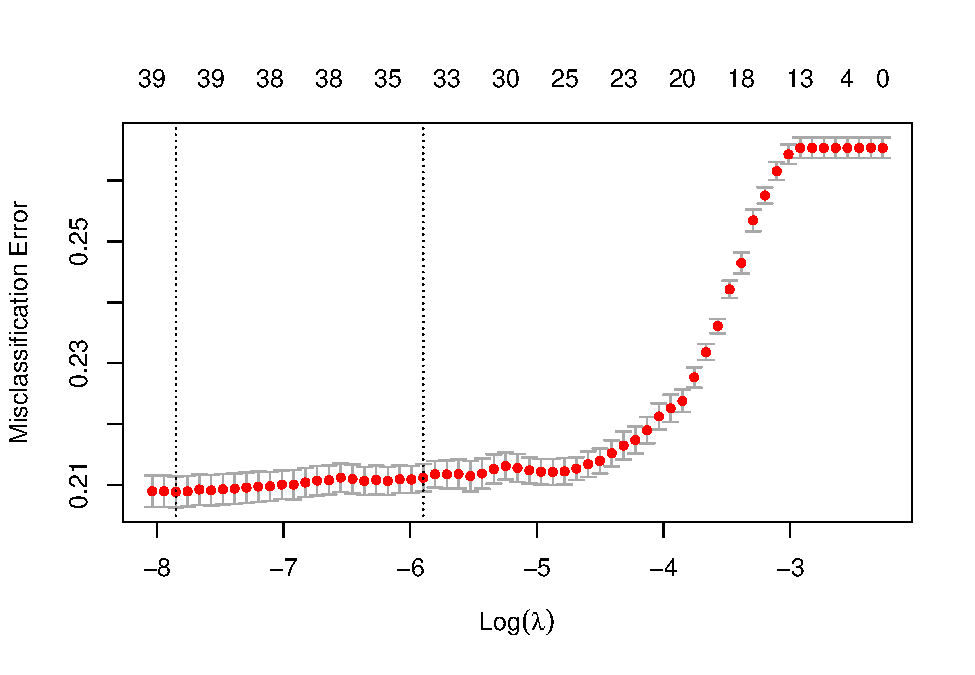
\includegraphics[keepaspectratio]{DATA_621_HW4_Group2_knit_files/figure-latex/unnamed-chunk-11-1.pdf}}

\begin{verbatim}
## 46 x 1 sparse Matrix of class "dgCMatrix"
##                                          s1
## (Intercept)                   -3.582686e-01
## BLUEBOOK_transformed          -2.136373e-01
## INCOME_transformed            -2.225871e-01
## MVR_PTS_transformed            2.411654e-01
## OLDCLAIM_transformed          -1.137712e-01
## TIF_transformed               -2.296326e-01
## TRAVTIME_transformed           2.600776e-01
## YOJ_transformed               -8.220575e-02
## CLM_FREQ_transformed           3.577001e-01
## CAR_AGE_transformed           -5.891536e-02
## SEX.F                          2.577099e-02
## SEX.M                         -7.644467e-13
## EDUCATION.L                   -2.319275e-01
## EDUCATION.Q                    2.413108e-01
## EDUCATION.C                    1.392531e-01
## JOBBlue Collar                 4.185922e-01
## JOBClerical                    4.744570e-01
## JOBDoctor                     -1.989135e-01
## JOBHome Maker                  1.945416e-01
## JOBLawyer                      3.270194e-01
## JOBManager                    -4.096388e-01
## JOBProfessional                2.179706e-01
## JOBStudent                     .           
## CAR_USECommercial              7.774901e-01
## CAR_USEPrivate                -3.667568e-12
## CAR_TYPEMinivan               -5.725101e-01
## CAR_TYPEPanel Truck            .           
## CAR_TYPEPickup                -4.678947e-02
## CAR_TYPESports Car             3.149258e-01
## CAR_TYPESUV                    1.373379e-01
## CAR_TYPEVan                    7.984963e-02
## URBANICITYHighly Rural/ Rural -2.459208e+00
## URBANICITYHighly Urban/ Urban  1.979274e-12
## HOME_VAL_CAT.Very Low         -9.471697e-03
## HOME_VAL_CAT.Low               .           
## HOME_VAL_CAT.Medium            1.179678e-02
## HOME_VAL_CAT.High             -1.294599e-02
## HOME_VAL_CAT.Missing           3.728283e-01
## RED_CAR.No                    -2.054552e-03
## RED_CAR.Yes                    .           
## REVOKED.No                    -8.701874e-01
## REVOKED.Yes                    9.253545e-13
## PARENT1.No                    -7.113841e-01
## PARENT1.Yes                    .           
## MSTATUS.No                     3.472215e-01
## MSTATUS.Yes                   -3.862138e-12
\end{verbatim}

\begin{verbatim}
## [1] "Best Lambda:  0.000323309244257453"
\end{verbatim}

The results from the model yield some notable insights. For example, the
variable CAR\_USECommercial shows a strong positive association with
crash likelihood---an intuitive finding, as commercial drivers may be
less cautious when the vehicle isn't personally owned, and they may also
spend more time on the road. Similarly, URBANICITYHighly Rural/Rural has
a strong negative correlation with crashes, which makes sense given the
lower traffic density in rural areas, reducing the chance of collisions.
As expected, REVOKED.No (i.e., not having a revoked license) is linked
to a reduced probability of being involved in a crash.

\paragraph{Model Comparison}\label{model-comparison}

We now run our three models on the test data and compare the results.

\begin{verbatim}
## Setting levels: control = 0, case = 1
\end{verbatim}

\begin{verbatim}
## Setting direction: controls < cases
\end{verbatim}

\begin{verbatim}
## Setting levels: control = 0, case = 1
\end{verbatim}

\begin{verbatim}
## Setting direction: controls < cases
\end{verbatim}

\begin{verbatim}
## Setting levels: control = 0, case = 1
\end{verbatim}

\begin{verbatim}
## Warning in roc.default(test_final$TARGET_FLAG, lasso_model_predictions):
## Deprecated use a matrix as predictor. Unexpected results may be produced,
## please pass a numeric vector.
\end{verbatim}

\begin{verbatim}
## Setting direction: controls < cases
\end{verbatim}

\begin{table}[H]
\centering\centering
\caption{\label{tab:unnamed-chunk-12}Comparison of Logistic Models}
\centering
\begin{tabular}[t]{l|r|r|r|r|r|r|r}
\hline
Model & RMSE & AIC & Accuracy & Precision & Recall & F1\_Score & ROC\_AUC\\
\hline
Model\_Transformed & 0.4653869 & 25514.47 & 0.7834150 & 0.3915228 & 0.6362245 & 0.4847425 & 0.7942114\\
\hline
Model\_Untransformed & 0.4638042 & 25464.04 & 0.7848856 & 0.4128728 & 0.6328200 & 0.4997150 & 0.7984942\\
\hline
Lasso Model & 0.4638923 & NA & 0.7848039 & 0.3946625 & 0.6403464 & 0.4883450 & 0.7929631\\
\hline
\end{tabular}
\end{table}

It's important to note that we haven't reported the AIC for the Lasso
model, as its use of regularization complicates the assumptions
underlying AIC calculations. That said, one of the most striking
observations is how similar the performance metrics are across all three
models.

The untransformed model shows the lowest RMSE, suggesting it yields the
smallest prediction error. It also has the lowest AIC, meaning it
performs best in terms of balancing model fit and complexity. When it
comes to classification metrics---accuracy, precision, and recall---the
untransformed model holds a slight lead in accuracy and precision, while
the Lasso model edges out in recall. This could be significant in
contexts where identifying true positives is especially important.

Interestingly, the second model (non-transformed, manually refined)
leads in both F1 score and ROC-AUC, indicating strong overall
performance and good class discrimination across various thresholds.

While the differences among the models are relatively small, the second
model stands out for its consistency across nearly all metrics. Although
it doesn't have the highest recall, its shortfall compared to the Lasso
model is minimal (only 0.0072004), and thus not particularly concerning.
Most importantly, the second model is \textbf{highly interpretable},
making it the preferred choice---especially in scenarios where
understanding the model's decision-making process is critical.

\textbf{Therefore, we select the second
model---``final\_non-transformed\_model''---as our final choice.}

\subsubsection{Multiple Linear
Regression}\label{multiple-linear-regression}

Up to this point, we've focused on modeling the likelihood of a car
crash and have chosen the most effective model for that task. We now
shift our attention to predicting the payout amount in cases where a
crash has occurred. To start, we'll manually select predictors based on
their correlation with the response variable and domain knowledge. We'll
then refine this initial model using a stepwise regression approach.
Finally, we'll compare the performance of both models---manual and
stepwise---using key evaluation metrics such as RMSE and R-squared to
determine which model more accurately predicts TARGET\_AMT.

\paragraph{Model 1}\label{model-1-1}

When selecting variables, it's reasonable to assume that predictors
which were significant in determining whether a crash occurred may also
be relevant in estimating the payout following a crash. We'll now put
that intuition to the test by evaluating their effectiveness in this new
context.

\begin{Shaded}
\begin{Highlighting}[]
\CommentTok{\#have to add back ticks or it just won\textquotesingle{}t work}
\NormalTok{predictors }\OtherTok{\textless{}{-}} \FunctionTok{c}\NormalTok{(}\StringTok{"KIDSDRIV"}\NormalTok{, }\StringTok{"AGE"}\NormalTok{, }\StringTok{"YOJ"}\NormalTok{, }\StringTok{"INCOME"}\NormalTok{, }\StringTok{"TRAVTIME"}\NormalTok{, }\StringTok{"BLUEBOOK"}\NormalTok{, }\StringTok{"TIF"}\NormalTok{,}
                \StringTok{"OLDCLAIM"}\NormalTok{, }\StringTok{"CLM\_FREQ"}\NormalTok{, }\StringTok{"MVR\_PTS"}\NormalTok{, }\StringTok{"EDUCATION.L"}\NormalTok{, }\StringTok{"EDUCATION.C"}\NormalTok{,}
                \StringTok{"\textasciigrave{}JOBBlue Collar\textasciigrave{}"}\NormalTok{, }\StringTok{"JOBClerical"}\NormalTok{, }\StringTok{"JOBDoctor"}\NormalTok{, }\StringTok{"JOBLawyer"}\NormalTok{,}
                \StringTok{"JOBManager"}\NormalTok{, }\StringTok{"JOBProfessional"}\NormalTok{, }\StringTok{"JOBStudent"}\NormalTok{, }\StringTok{"CAR\_USECommercial"}\NormalTok{,}
                \StringTok{"CAR\_TYPEMinivan"}\NormalTok{, }\StringTok{"\textasciigrave{}CAR\_TYPEPanel Truck\textasciigrave{}"}\NormalTok{, }\StringTok{"CAR\_TYPEPickup"}\NormalTok{,}
                \StringTok{"\textasciigrave{}CAR\_TYPESports Car\textasciigrave{}"}\NormalTok{, }\StringTok{"\textasciigrave{}URBANICITYHighly Rural/ Rural\textasciigrave{}"}\NormalTok{,}
                \StringTok{"\textasciigrave{}HOME\_VAL\_CAT.Very Low\textasciigrave{}"}\NormalTok{, }\StringTok{"HOME\_VAL\_CAT.Medium"}\NormalTok{, }\StringTok{"HOME\_VAL\_CAT.High"}\NormalTok{,}
                \StringTok{"HOME\_VAL\_CAT.Missing"}\NormalTok{, }\StringTok{"REVOKED.No"}\NormalTok{, }\StringTok{"PARENT1.No"}\NormalTok{, }\StringTok{"MSTATUS.No"}\NormalTok{)}

\NormalTok{formula }\OtherTok{\textless{}{-}} \FunctionTok{as.formula}\NormalTok{(}\FunctionTok{paste}\NormalTok{(}\StringTok{"TARGET\_AMT \textasciitilde{}"}\NormalTok{, }\FunctionTok{paste}\NormalTok{(predictors, }\AttributeTok{collapse=}\StringTok{" + "}\NormalTok{)))}
\NormalTok{mlr1 }\OtherTok{\textless{}{-}} \FunctionTok{lm}\NormalTok{(formula, }\AttributeTok{data =}\NormalTok{ train\_final)}
\FunctionTok{summary}\NormalTok{(mlr1)}
\end{Highlighting}
\end{Shaded}

\begin{verbatim}
## 
## Call:
## lm(formula = formula, data = train_final)
## 
## Residuals:
##    Min     1Q Median     3Q    Max 
##  -5661  -1775   -784    381 103949 
## 
## Coefficients:
##                                  Estimate Std. Error t value Pr(>|t|)    
## (Intercept)                      2810.494    177.476  15.836  < 2e-16 ***
## KIDSDRIV                          217.511     29.002   7.500 6.58e-14 ***
## AGE                                35.855     31.173   1.150 0.250067    
## YOJ                                 4.837     29.072   0.166 0.867849    
## INCOME                           -180.845     46.505  -3.889 0.000101 ***
## TRAVTIME                          234.589     28.267   8.299  < 2e-16 ***
## BLUEBOOK                           27.282     33.866   0.806 0.420490    
## TIF                              -215.067     27.989  -7.684 1.59e-14 ***
## OLDCLAIM                           43.167     37.785   1.142 0.253280    
## CLM_FREQ                          136.293     38.112   3.576 0.000349 ***
## MVR_PTS                           208.682     30.575   6.825 8.96e-12 ***
## EDUCATION.L                      -583.498    126.675  -4.606 4.12e-06 ***
## EDUCATION.C                        40.731     70.617   0.577 0.564087    
## `JOBBlue Collar`                  -31.867    125.246  -0.254 0.799164    
## JOBClerical                        49.615    122.464   0.405 0.685377    
## JOBDoctor                        -376.141    196.140  -1.918 0.055156 .  
## JOBLawyer                         110.513    131.855   0.838 0.401957    
## JOBManager                       -924.749    119.735  -7.723 1.17e-14 ***
## JOBProfessional                   111.068    117.848   0.942 0.345960    
## JOBStudent                       -239.272    147.475  -1.622 0.104715    
## CAR_USECommercial                 954.853     85.347  11.188  < 2e-16 ***
## CAR_TYPEMinivan                  -577.629     72.456  -7.972 1.62e-15 ***
## `CAR_TYPEPanel Truck`            -509.313    132.321  -3.849 0.000119 ***
## CAR_TYPEPickup                   -209.171     85.318  -2.452 0.014226 *  
## `CAR_TYPESports Car`              114.244     97.386   1.173 0.240765    
## `URBANICITYHighly Rural/ Rural` -1881.873     76.195 -24.698  < 2e-16 ***
## `HOME_VAL_CAT.Very Low`          -267.017    107.529  -2.483 0.013026 *  
## HOME_VAL_CAT.Medium              -234.421    102.376  -2.290 0.022040 *  
## HOME_VAL_CAT.High                -196.478    123.380  -1.592 0.111294    
## HOME_VAL_CAT.Missing              116.660    103.714   1.125 0.260673    
## REVOKED.No                       -312.336     89.595  -3.486 0.000491 ***
## PARENT1.No                       -838.618    101.260  -8.282  < 2e-16 ***
## MSTATUS.No                        404.501     79.407   5.094 3.53e-07 ***
## ---
## Signif. codes:  0 '***' 0.001 '**' 0.01 '*' 0.05 '.' 0.1 ' ' 1
## 
## Residual standard error: 4717 on 28532 degrees of freedom
## Multiple R-squared:  0.06831,    Adjusted R-squared:  0.06726 
## F-statistic: 65.37 on 32 and 28532 DF,  p-value: < 2.2e-16
\end{verbatim}

While the overall model is statistically significant, the Adjusted
R-squared remains quite low, indicating limited explanatory power.
However, it's important to emphasize that our primary interest lies in
predicting payouts only when a crash has actually occurred---that is,
when \textbf{TARGET\_FLAG =1}. In all other cases, the payout is simply
zero. With this in mind, let's assess model performance by multiplying
the predicted values by the TARGET\_FLAG, effectively filtering
predictions to only those instances where a payout would apply.

\begin{verbatim}
## 
## Call:
## lm(formula = formula, data = train_final)
## 
## Residuals:
##    Min     1Q Median     3Q    Max 
##  -9772   -407    -50    182  98182 
## 
## Coefficients:
##                                               Estimate Std. Error t value
## (Intercept)                                  1970.4638   158.0469  12.468
## KIDSDRIV:TARGET_FLAG0                         -28.4489    32.5642  -0.874
## KIDSDRIV:TARGET_FLAG1                         144.0430    40.8194   3.529
## TARGET_FLAG0:AGE                               51.2883    32.7545   1.566
## TARGET_FLAG1:AGE                              176.7488    48.5476   3.641
## TARGET_FLAG0:YOJ                              -21.6436    29.0844  -0.744
## TARGET_FLAG1:YOJ                               83.1716    51.9167   1.602
## TARGET_FLAG0:INCOME                            87.3026    46.4044   1.881
## TARGET_FLAG1:INCOME                          -292.3788    82.4195  -3.547
## TARGET_FLAG0:TRAVTIME                          14.0717    28.6553   0.491
## TARGET_FLAG1:TRAVTIME                          70.4384    49.3442   1.427
## TARGET_FLAG0:BLUEBOOK                          -0.4141    34.0365  -0.012
## TARGET_FLAG1:BLUEBOOK                         774.2379    60.2575  12.849
## TARGET_FLAG0:TIF                               -2.1602    28.3742  -0.076
## TARGET_FLAG1:TIF                             -211.0707    48.6265  -4.341
## TARGET_FLAG0:OLDCLAIM                          34.4627    42.4430   0.812
## TARGET_FLAG1:OLDCLAIM                        -612.3448    53.2366 -11.502
## TARGET_FLAG0:CLM_FREQ                         -24.1086    42.3402  -0.569
## TARGET_FLAG1:CLM_FREQ                         323.1709    54.6081   5.918
## TARGET_FLAG0:MVR_PTS                          -11.1591    33.2745  -0.335
## TARGET_FLAG1:MVR_PTS                          231.6953    45.1832   5.128
## TARGET_FLAG0:EDUCATION.L                     -115.9451   129.0330  -0.899
## TARGET_FLAG1:EDUCATION.L                       43.1633   215.6166   0.200
## TARGET_FLAG0:EDUCATION.C                        1.2804    72.4887   0.018
## TARGET_FLAG1:EDUCATION.C                     -357.6296   118.3050  -3.023
## TARGET_FLAG0:`JOBBlue Collar`                -419.4723   126.7119  -3.310
## TARGET_FLAG1:`JOBBlue Collar`                 492.8868   199.1576   2.475
## TARGET_FLAG0:JOBClerical                     -495.8922   122.8803  -4.036
## TARGET_FLAG1:JOBClerical                      858.8200   190.6683   4.504
## TARGET_FLAG0:JOBDoctor                       -366.2016   187.5902  -1.952
## TARGET_FLAG1:JOBDoctor                       -805.2224   428.7391  -1.878
## TARGET_FLAG0:JOBLawyer                       -435.4200   128.7557  -3.382
## TARGET_FLAG1:JOBLawyer                       1208.2596   236.9814   5.099
## TARGET_FLAG0:JOBManager                      -455.1447   115.1203  -3.954
## TARGET_FLAG1:JOBManager                      -925.9004   229.4867  -4.035
## TARGET_FLAG0:JOBProfessional                 -451.0646   116.0287  -3.888
## TARGET_FLAG1:JOBProfessional                 1763.1868   195.9964   8.996
## TARGET_FLAG0:JOBStudent                      -314.3454   155.4414  -2.022
## TARGET_FLAG1:JOBStudent                       508.7804   226.4465   2.247
## TARGET_FLAG0:CAR_USECommercial               -100.4509    88.8942  -1.130
## TARGET_FLAG1:CAR_USECommercial               1252.4709   139.2479   8.995
## TARGET_FLAG0:CAR_TYPEMinivan                  -85.6880    71.6873  -1.195
## TARGET_FLAG1:CAR_TYPEMinivan                  258.2139   138.6647   1.862
## TARGET_FLAG0:`CAR_TYPEPanel Truck`           -109.2627   136.5449  -0.800
## TARGET_FLAG1:`CAR_TYPEPanel Truck`           -785.3666   217.8553  -3.605
## TARGET_FLAG0:CAR_TYPEPickup                   -93.7736    88.5081  -1.059
## TARGET_FLAG1:CAR_TYPEPickup                   -60.0866   138.0882  -0.435
## TARGET_FLAG0:`CAR_TYPESports Car`            -125.2667   103.3371  -1.212
## TARGET_FLAG1:`CAR_TYPESports Car`              66.6815   147.6361   0.452
## TARGET_FLAG0:`URBANICITYHighly Rural/ Rural`  -73.8745    74.7444  -0.988
## TARGET_FLAG1:`URBANICITYHighly Rural/ Rural` -734.6768   220.3300  -3.334
## TARGET_FLAG0:`HOME_VAL_CAT.Very Low`         -354.4719   107.0368  -3.312
## TARGET_FLAG1:`HOME_VAL_CAT.Very Low`         -271.6505   176.7837  -1.537
## TARGET_FLAG0:HOME_VAL_CAT.Medium             -342.4793   100.6463  -3.403
## TARGET_FLAG1:HOME_VAL_CAT.Medium              -22.1083   177.4310  -0.125
## TARGET_FLAG0:HOME_VAL_CAT.High               -448.6537   119.8643  -3.743
## TARGET_FLAG1:HOME_VAL_CAT.High                737.6524   231.0058   3.193
## TARGET_FLAG0:HOME_VAL_CAT.Missing            -329.6272   104.8792  -3.143
## TARGET_FLAG1:HOME_VAL_CAT.Missing            -250.2335   166.2395  -1.505
## TARGET_FLAG0:REVOKED.No                      -482.8913    97.2306  -4.966
## TARGET_FLAG1:REVOKED.No                      2409.2792   122.3963  19.684
## TARGET_FLAG0:PARENT1.No                      -684.8673   106.7114  -6.418
## TARGET_FLAG1:PARENT1.No                       457.7510   131.8742   3.471
## TARGET_FLAG0:MSTATUS.No                      -254.6131    78.9919  -3.223
## TARGET_FLAG1:MSTATUS.No                      1114.8123   133.7245   8.337
##                                              Pr(>|t|)    
## (Intercept)                                   < 2e-16 ***
## KIDSDRIV:TARGET_FLAG0                        0.382330    
## KIDSDRIV:TARGET_FLAG1                        0.000418 ***
## TARGET_FLAG0:AGE                             0.117398    
## TARGET_FLAG1:AGE                             0.000272 ***
## TARGET_FLAG0:YOJ                             0.456784    
## TARGET_FLAG1:YOJ                             0.109162    
## TARGET_FLAG0:INCOME                          0.059936 .  
## TARGET_FLAG1:INCOME                          0.000390 ***
## TARGET_FLAG0:TRAVTIME                        0.623383    
## TARGET_FLAG1:TRAVTIME                        0.153449    
## TARGET_FLAG0:BLUEBOOK                        0.990294    
## TARGET_FLAG1:BLUEBOOK                         < 2e-16 ***
## TARGET_FLAG0:TIF                             0.939315    
## TARGET_FLAG1:TIF                             1.43e-05 ***
## TARGET_FLAG0:OLDCLAIM                        0.416812    
## TARGET_FLAG1:OLDCLAIM                         < 2e-16 ***
## TARGET_FLAG0:CLM_FREQ                        0.569088    
## TARGET_FLAG1:CLM_FREQ                        3.30e-09 ***
## TARGET_FLAG0:MVR_PTS                         0.737352    
## TARGET_FLAG1:MVR_PTS                         2.95e-07 ***
## TARGET_FLAG0:EDUCATION.L                     0.368890    
## TARGET_FLAG1:EDUCATION.L                     0.841337    
## TARGET_FLAG0:EDUCATION.C                     0.985908    
## TARGET_FLAG1:EDUCATION.C                     0.002506 ** 
## TARGET_FLAG0:`JOBBlue Collar`                0.000933 ***
## TARGET_FLAG1:`JOBBlue Collar`                0.013335 *  
## TARGET_FLAG0:JOBClerical                     5.46e-05 ***
## TARGET_FLAG1:JOBClerical                     6.69e-06 ***
## TARGET_FLAG0:JOBDoctor                       0.050932 .  
## TARGET_FLAG1:JOBDoctor                       0.060375 .  
## TARGET_FLAG0:JOBLawyer                       0.000721 ***
## TARGET_FLAG1:JOBLawyer                       3.44e-07 ***
## TARGET_FLAG0:JOBManager                      7.72e-05 ***
## TARGET_FLAG1:JOBManager                      5.48e-05 ***
## TARGET_FLAG0:JOBProfessional                 0.000102 ***
## TARGET_FLAG1:JOBProfessional                  < 2e-16 ***
## TARGET_FLAG0:JOBStudent                      0.043157 *  
## TARGET_FLAG1:JOBStudent                      0.024660 *  
## TARGET_FLAG0:CAR_USECommercial               0.258484    
## TARGET_FLAG1:CAR_USECommercial                < 2e-16 ***
## TARGET_FLAG0:CAR_TYPEMinivan                 0.231979    
## TARGET_FLAG1:CAR_TYPEMinivan                 0.062593 .  
## TARGET_FLAG0:`CAR_TYPEPanel Truck`           0.423604    
## TARGET_FLAG1:`CAR_TYPEPanel Truck`           0.000313 ***
## TARGET_FLAG0:CAR_TYPEPickup                  0.289385    
## TARGET_FLAG1:CAR_TYPEPickup                  0.663470    
## TARGET_FLAG0:`CAR_TYPESports Car`            0.225440    
## TARGET_FLAG1:`CAR_TYPESports Car`            0.651516    
## TARGET_FLAG0:`URBANICITYHighly Rural/ Rural` 0.322984    
## TARGET_FLAG1:`URBANICITYHighly Rural/ Rural` 0.000856 ***
## TARGET_FLAG0:`HOME_VAL_CAT.Very Low`         0.000929 ***
## TARGET_FLAG1:`HOME_VAL_CAT.Very Low`         0.124396    
## TARGET_FLAG0:HOME_VAL_CAT.Medium             0.000668 ***
## TARGET_FLAG1:HOME_VAL_CAT.Medium             0.900840    
## TARGET_FLAG0:HOME_VAL_CAT.High               0.000182 ***
## TARGET_FLAG1:HOME_VAL_CAT.High               0.001408 ** 
## TARGET_FLAG0:HOME_VAL_CAT.Missing            0.001674 ** 
## TARGET_FLAG1:HOME_VAL_CAT.Missing            0.132269    
## TARGET_FLAG0:REVOKED.No                      6.86e-07 ***
## TARGET_FLAG1:REVOKED.No                       < 2e-16 ***
## TARGET_FLAG0:PARENT1.No                      1.40e-10 ***
## TARGET_FLAG1:PARENT1.No                      0.000519 ***
## TARGET_FLAG0:MSTATUS.No                      0.001269 ** 
## TARGET_FLAG1:MSTATUS.No                       < 2e-16 ***
## ---
## Signif. codes:  0 '***' 0.001 '**' 0.01 '*' 0.05 '.' 0.1 ' ' 1
## 
## Residual standard error: 4107 on 28500 degrees of freedom
## Multiple R-squared:  0.2945, Adjusted R-squared:  0.2929 
## F-statistic: 185.9 on 64 and 28500 DF,  p-value: < 2.2e-16
\end{verbatim}

This adjusted model shows a notable improvement and aligns well with
intuition---it ensures that only cases predicted as crashes yield a
positive \textbf{TARGET\_AMT}. This logic adds a layer of practical
accuracy to our predictions. That said, we'll now explore whether we can
retain this intuitive structure while enhancing the model's performance
by refining our set of predictors.

\paragraph{Model 2}\label{model-2-1}

Once again, we plan to incorporate TARGET\_FLAG into our modeling
strategy. However, this time we'll apply an automated stepwise
regression approach. This iterative process evaluates predictors based
on their statistical significance, systematically adding or removing
variables to arrive at the most optimal model fit.

From the stepwise process, we learn that our best model is:

TARGET\_AMT \textasciitilde{} AGE:TARGET\_FLAG + TARGET\_FLAG:INCOME +
TARGET\_FLAG:TIF + TARGET\_FLAG:YOJ + TARGET\_FLAG:HOMEKIDS +
TARGET\_FLAG:CLM\_FREQ + TARGET\_FLAG:CAR\_AGE + TARGET\_FLAG:OLDCLAIM +
TARGET\_FLAG:BLUEBOOK\_transformed + TARGET\_FLAG:INCOME\_transformed +
TARGET\_FLAG:MVR\_PTS\_transformed + TARGET\_FLAG:TIF\_transformed +
TARGET\_FLAG:YOJ\_transformed + TARGET\_FLAG:CLM\_FREQ\_transformed +
TARGET\_FLAG:CAR\_AGE\_transformed + TARGET\_FLAG:SEX.F +
TARGET\_FLAG:SEX.M + TARGET\_FLAG:EDUCATION.L + TARGET\_FLAG:EDUCATION.Q
+ TARGET\_FLAG:\texttt{EDUCATION\^{}4} +
TARGET\_FLAG:\texttt{JOBBlue\ Collar} + TARGET\_FLAG:JOBClerical +
TARGET\_FLAG:JOBDoctor + TARGET\_FLAG:\texttt{JOBHome\ Maker} +
TARGET\_FLAG:JOBLawyer + TARGET\_FLAG:JOBManager +
TARGET\_FLAG:JOBStudent + TARGET\_FLAG:CAR\_USECommercial +
TARGET\_FLAG:\texttt{CAR\_TYPEPanel\ Truck} +
TARGET\_FLAG:CAR\_TYPEPickup +
TARGET\_FLAG:\texttt{CAR\_TYPESports\ Car} + TARGET\_FLAG:CAR\_TYPESUV +
TARGET\_FLAG:\texttt{URBANICITYHighly\ Rural/\ Rural} +
TARGET\_FLAG:HOME\_VAL\_CAT.Low + TARGET\_FLAG:HOME\_VAL\_CAT.Medium +
TARGET\_FLAG:HOME\_VAL\_CAT.High + TARGET\_FLAG:REVOKED.No +
TARGET\_FLAG:PARENT1.No + TARGET\_FLAG:MSTATUS.No

Now, this seems quite involved. But it's worth repeating--the constant
presence of \texttt{TARGET\_FLAG} is simply to guarantee that only
observations with a \texttt{TARGET\_FLAG} of 1 will have a non-zero
value for \texttt{TARGET\_AMT.} Let us now print the summary:

\begin{verbatim}
## 
## Call:
## lm(formula = best_stepwise_formula, data = train_final)
## 
## Residuals:
##    Min     1Q Median     3Q    Max 
##  -9680      0      0      0  98577 
## 
## Coefficients: (1 not defined because of singularities)
##                                                Estimate Std. Error t value
## (Intercept)                                   4.134e+03  3.963e+02  10.431
## AGE:TARGET_FLAG0                              3.526e-11  3.534e+01   0.000
## AGE:TARGET_FLAG1                              2.918e+02  5.137e+01   5.682
## TARGET_FLAG0:INCOME                           7.154e-12  5.735e+01   0.000
## TARGET_FLAG1:INCOME                           3.948e+02  1.247e+02   3.166
## TARGET_FLAG0:TIF                             -1.241e-11  6.672e+01   0.000
## TARGET_FLAG1:TIF                             -6.371e+02  1.329e+02  -4.794
## TARGET_FLAG0:YOJ                              6.131e-12  3.503e+01   0.000
## TARGET_FLAG1:YOJ                             -1.881e+02  5.945e+01  -3.164
## TARGET_FLAG0:HOMEKIDS                        -2.727e-12  3.864e+01   0.000
## TARGET_FLAG1:HOMEKIDS                         3.126e+02  6.182e+01   5.057
## TARGET_FLAG0:CLM_FREQ                        -1.942e-12  1.389e+02   0.000
## TARGET_FLAG1:CLM_FREQ                        -6.856e+02  1.735e+02  -3.951
## TARGET_FLAG0:CAR_AGE                         -2.095e-11  2.042e+02   0.000
## TARGET_FLAG1:CAR_AGE                         -3.420e+03  3.594e+02  -9.518
## TARGET_FLAG0:OLDCLAIM                        -4.013e-12  4.605e+01   0.000
## TARGET_FLAG1:OLDCLAIM                        -6.453e+02  5.971e+01 -10.806
## TARGET_FLAG0:BLUEBOOK_transformed             2.973e-12  3.846e+01   0.000
## TARGET_FLAG1:BLUEBOOK_transformed             9.770e+02  6.426e+01  15.205
## TARGET_FLAG0:INCOME_transformed               8.900e-12  7.218e+01   0.000
## TARGET_FLAG1:INCOME_transformed              -9.076e+02  1.502e+02  -6.044
## TARGET_FLAG0:MVR_PTS_transformed              8.522e-12  3.570e+01   0.000
## TARGET_FLAG1:MVR_PTS_transformed              2.356e+02  5.059e+01   4.657
## TARGET_FLAG0:TIF_transformed                  8.488e-12  6.719e+01   0.000
## TARGET_FLAG1:TIF_transformed                  4.480e+02  1.310e+02   3.419
## TARGET_FLAG0:YOJ_transformed                 -1.099e-11  4.389e+01   0.000
## TARGET_FLAG1:YOJ_transformed                  2.321e+02  6.503e+01   3.569
## TARGET_FLAG0:CLM_FREQ_transformed            -7.629e-12  2.115e+02   0.000
## TARGET_FLAG1:CLM_FREQ_transformed             1.554e+03  2.761e+02   5.629
## TARGET_FLAG0:CAR_AGE_transformed              1.997e-11  2.009e+02   0.000
## TARGET_FLAG1:CAR_AGE_transformed              3.124e+03  3.348e+02   9.330
## TARGET_FLAG0:SEX.F                           -4.134e+03  4.778e+02  -8.652
## TARGET_FLAG1:SEX.F                           -1.095e+03  1.617e+02  -6.770
## TARGET_FLAG0:SEX.M                           -4.134e+03  4.744e+02  -8.714
## TARGET_FLAG1:SEX.M                                   NA         NA      NA
## TARGET_FLAG0:EDUCATION.L                     -4.836e-11  1.468e+02   0.000
## TARGET_FLAG1:EDUCATION.L                      1.451e+03  2.653e+02   5.470
## TARGET_FLAG0:EDUCATION.Q                     -2.636e-11  8.260e+01   0.000
## TARGET_FLAG1:EDUCATION.Q                      1.682e+03  1.426e+02  11.793
## TARGET_FLAG0:`EDUCATION^4`                   -1.692e-12  6.223e+01   0.000
## TARGET_FLAG1:`EDUCATION^4`                   -4.282e+02  1.036e+02  -4.133
## TARGET_FLAG0:`JOBBlue Collar`                -2.070e-12  1.133e+02   0.000
## TARGET_FLAG1:`JOBBlue Collar`                -1.581e+03  1.808e+02  -8.743
## TARGET_FLAG0:JOBClerical                      9.629e-12  1.200e+02   0.000
## TARGET_FLAG1:JOBClerical                     -1.696e+03  1.989e+02  -8.530
## TARGET_FLAG0:JOBDoctor                        7.652e-11  1.894e+02   0.000
## TARGET_FLAG1:JOBDoctor                       -3.889e+03  4.418e+02  -8.801
## TARGET_FLAG0:`JOBHome Maker`                  2.536e-11  1.537e+02   0.000
## TARGET_FLAG1:`JOBHome Maker`                 -1.801e+03  2.776e+02  -6.487
## TARGET_FLAG0:JOBLawyer                        4.249e-11  1.193e+02   0.000
## TARGET_FLAG1:JOBLawyer                       -1.027e+03  2.443e+02  -4.202
## TARGET_FLAG0:JOBManager                       2.341e-11  9.928e+01   0.000
## TARGET_FLAG1:JOBManager                      -2.727e+03  2.215e+02 -12.312
## TARGET_FLAG0:JOBStudent                       1.440e-11  1.609e+02   0.000
## TARGET_FLAG1:JOBStudent                      -1.539e+03  2.575e+02  -5.977
## TARGET_FLAG0:CAR_USECommercial                1.316e-11  8.833e+01   0.000
## TARGET_FLAG1:CAR_USECommercial                7.899e+02  1.417e+02   5.573
## TARGET_FLAG0:`CAR_TYPEPanel Truck`            1.988e-11  1.368e+02   0.000
## TARGET_FLAG1:`CAR_TYPEPanel Truck`           -1.693e+03  2.227e+02  -7.604
## TARGET_FLAG0:CAR_TYPEPickup                   1.216e-11  8.910e+01   0.000
## TARGET_FLAG1:CAR_TYPEPickup                  -3.087e+02  1.501e+02  -2.056
## TARGET_FLAG0:`CAR_TYPESports Car`             9.077e-12  1.221e+02   0.000
## TARGET_FLAG1:`CAR_TYPESports Car`             5.371e+02  2.119e+02   2.534
## TARGET_FLAG0:CAR_TYPESUV                      8.935e-12  9.599e+01   0.000
## TARGET_FLAG1:CAR_TYPESUV                      6.841e+02  1.846e+02   3.706
## TARGET_FLAG0:`URBANICITYHighly Rural/ Rural` -2.260e-12  7.443e+01   0.000
## TARGET_FLAG1:`URBANICITYHighly Rural/ Rural` -7.216e+02  2.170e+02  -3.324
## TARGET_FLAG0:HOME_VAL_CAT.Low                 5.760e-12  9.213e+01   0.000
## TARGET_FLAG1:HOME_VAL_CAT.Low                 1.293e+03  1.587e+02   8.147
## TARGET_FLAG0:HOME_VAL_CAT.Medium              7.784e-12  9.033e+01   0.000
## TARGET_FLAG1:HOME_VAL_CAT.Medium              4.766e+02  1.589e+02   2.999
## TARGET_FLAG0:HOME_VAL_CAT.High                9.023e-12  1.106e+02   0.000
## TARGET_FLAG1:HOME_VAL_CAT.High                7.987e+02  2.184e+02   3.657
## TARGET_FLAG0:REVOKED.No                      -2.135e-12  9.999e+01   0.000
## TARGET_FLAG1:REVOKED.No                       1.895e+03  1.305e+02  14.517
## TARGET_FLAG0:PARENT1.No                      -1.404e-11  1.219e+02   0.000
## TARGET_FLAG1:PARENT1.No                      -3.940e+02  1.663e+02  -2.369
## TARGET_FLAG0:MSTATUS.No                      -1.373e-11  7.713e+01   0.000
## TARGET_FLAG1:MSTATUS.No                       7.713e+02  1.363e+02   5.659
##                                              Pr(>|t|)    
## (Intercept)                                   < 2e-16 ***
## AGE:TARGET_FLAG0                             1.000000    
## AGE:TARGET_FLAG1                             1.35e-08 ***
## TARGET_FLAG0:INCOME                          1.000000    
## TARGET_FLAG1:INCOME                          0.001546 ** 
## TARGET_FLAG0:TIF                             1.000000    
## TARGET_FLAG1:TIF                             1.64e-06 ***
## TARGET_FLAG0:YOJ                             1.000000    
## TARGET_FLAG1:YOJ                             0.001556 ** 
## TARGET_FLAG0:HOMEKIDS                        1.000000    
## TARGET_FLAG1:HOMEKIDS                        4.28e-07 ***
## TARGET_FLAG0:CLM_FREQ                        1.000000    
## TARGET_FLAG1:CLM_FREQ                        7.80e-05 ***
## TARGET_FLAG0:CAR_AGE                         1.000000    
## TARGET_FLAG1:CAR_AGE                          < 2e-16 ***
## TARGET_FLAG0:OLDCLAIM                        1.000000    
## TARGET_FLAG1:OLDCLAIM                         < 2e-16 ***
## TARGET_FLAG0:BLUEBOOK_transformed            1.000000    
## TARGET_FLAG1:BLUEBOOK_transformed             < 2e-16 ***
## TARGET_FLAG0:INCOME_transformed              1.000000    
## TARGET_FLAG1:INCOME_transformed              1.52e-09 ***
## TARGET_FLAG0:MVR_PTS_transformed             1.000000    
## TARGET_FLAG1:MVR_PTS_transformed             3.23e-06 ***
## TARGET_FLAG0:TIF_transformed                 1.000000    
## TARGET_FLAG1:TIF_transformed                 0.000629 ***
## TARGET_FLAG0:YOJ_transformed                 1.000000    
## TARGET_FLAG1:YOJ_transformed                 0.000359 ***
## TARGET_FLAG0:CLM_FREQ_transformed            1.000000    
## TARGET_FLAG1:CLM_FREQ_transformed            1.83e-08 ***
## TARGET_FLAG0:CAR_AGE_transformed             1.000000    
## TARGET_FLAG1:CAR_AGE_transformed              < 2e-16 ***
## TARGET_FLAG0:SEX.F                            < 2e-16 ***
## TARGET_FLAG1:SEX.F                           1.31e-11 ***
## TARGET_FLAG0:SEX.M                            < 2e-16 ***
## TARGET_FLAG1:SEX.M                                 NA    
## TARGET_FLAG0:EDUCATION.L                     1.000000    
## TARGET_FLAG1:EDUCATION.L                     4.55e-08 ***
## TARGET_FLAG0:EDUCATION.Q                     1.000000    
## TARGET_FLAG1:EDUCATION.Q                      < 2e-16 ***
## TARGET_FLAG0:`EDUCATION^4`                   1.000000    
## TARGET_FLAG1:`EDUCATION^4`                   3.59e-05 ***
## TARGET_FLAG0:`JOBBlue Collar`                1.000000    
## TARGET_FLAG1:`JOBBlue Collar`                 < 2e-16 ***
## TARGET_FLAG0:JOBClerical                     1.000000    
## TARGET_FLAG1:JOBClerical                      < 2e-16 ***
## TARGET_FLAG0:JOBDoctor                       1.000000    
## TARGET_FLAG1:JOBDoctor                        < 2e-16 ***
## TARGET_FLAG0:`JOBHome Maker`                 1.000000    
## TARGET_FLAG1:`JOBHome Maker`                 8.91e-11 ***
## TARGET_FLAG0:JOBLawyer                       1.000000    
## TARGET_FLAG1:JOBLawyer                       2.65e-05 ***
## TARGET_FLAG0:JOBManager                      1.000000    
## TARGET_FLAG1:JOBManager                       < 2e-16 ***
## TARGET_FLAG0:JOBStudent                      1.000000    
## TARGET_FLAG1:JOBStudent                      2.30e-09 ***
## TARGET_FLAG0:CAR_USECommercial               1.000000    
## TARGET_FLAG1:CAR_USECommercial               2.53e-08 ***
## TARGET_FLAG0:`CAR_TYPEPanel Truck`           1.000000    
## TARGET_FLAG1:`CAR_TYPEPanel Truck`           2.97e-14 ***
## TARGET_FLAG0:CAR_TYPEPickup                  1.000000    
## TARGET_FLAG1:CAR_TYPEPickup                  0.039787 *  
## TARGET_FLAG0:`CAR_TYPESports Car`            1.000000    
## TARGET_FLAG1:`CAR_TYPESports Car`            0.011276 *  
## TARGET_FLAG0:CAR_TYPESUV                     1.000000    
## TARGET_FLAG1:CAR_TYPESUV                     0.000211 ***
## TARGET_FLAG0:`URBANICITYHighly Rural/ Rural` 1.000000    
## TARGET_FLAG1:`URBANICITYHighly Rural/ Rural` 0.000887 ***
## TARGET_FLAG0:HOME_VAL_CAT.Low                1.000000    
## TARGET_FLAG1:HOME_VAL_CAT.Low                3.89e-16 ***
## TARGET_FLAG0:HOME_VAL_CAT.Medium             1.000000    
## TARGET_FLAG1:HOME_VAL_CAT.Medium             0.002709 ** 
## TARGET_FLAG0:HOME_VAL_CAT.High               1.000000    
## TARGET_FLAG1:HOME_VAL_CAT.High               0.000256 ***
## TARGET_FLAG0:REVOKED.No                      1.000000    
## TARGET_FLAG1:REVOKED.No                       < 2e-16 ***
## TARGET_FLAG0:PARENT1.No                      1.000000    
## TARGET_FLAG1:PARENT1.No                      0.017840 *  
## TARGET_FLAG0:MSTATUS.No                      1.000000    
## TARGET_FLAG1:MSTATUS.No                      1.54e-08 ***
## ---
## Signif. codes:  0 '***' 0.001 '**' 0.01 '*' 0.05 '.' 0.1 ' ' 1
## 
## Residual standard error: 4053 on 28487 degrees of freedom
## Multiple R-squared:  0.3132, Adjusted R-squared:  0.3114 
## F-statistic: 168.7 on 77 and 28487 DF,  p-value: < 2.2e-16
\end{verbatim}

\paragraph{Model Comparison}\label{model-comparison-1}

We now have two models that share a key similarity but differ in how
they were built. Both models incorporate \textbf{TARGET\_FLAG} to guide
predictions of \textbf{TARGET\_AMT}, a strategy we've intentionally
preserved due to its clear relevance. The primary distinction lies in
the variable selection process: the first model was manually curated
using insights from our best logistic regression model, while the second
was generated through an automated stepwise regression approach.
Naturally, it's essential to compare their performance to determine
which model is more effective.

We summarize key metrics below:

\begin{table}[H]
\centering\centering
\caption{\label{tab:unnamed-chunk-14}Multiple Linear Regression Models Comparison}
\centering
\begin{tabular}[t]{l|r|r|r}
\hline
Model & RMSE & MAE & R\_squared\\
\hline
Best Stepwise & 3637.063 & 988.030 & 0.2676403\\
\hline
MLR2 & 3598.572 & 1129.521 & 0.2830594\\
\hline
\end{tabular}
\end{table}

The comparison table offers valuable insight for selecting our final
model. While MLR2 has a marginally lower RMSE and a slightly higher
R-squared, it's important to emphasize that in this context, RMSE and
especially MAE carry more weight than R-squared. Since our primary goal
is to minimize financial prediction errors, lower RMSE and MAE values
indicate more reliable payout estimates.

Although Best Stepwise slightly underperforms on RMSE and R-squared, it
delivers a significantly lower MAE, which reflects the average
prediction error. This makes it particularly relevant for applications
where accuracy in dollar amounts is crucial. Furthermore, in this case,
predictive accuracy outweighs model simplicity, meaning interpretability
is not the top priority.

Given these factors, despite MLR2's slight edge in two metrics, the much
stronger MAE performance of Best Stepwise justifies its selection as the
final model.

\subsubsection{Predictions}\label{predictions}

With our final models selected, we're now prepared to generate
predictions using the evaluation dataset. However, this process is
slightly more involved, as our second model's predictions depend on the
output of the first. The complete prediction workflow is outlined below:

\begin{table}[H]
\centering\centering
\caption{\label{tab:unnamed-chunk-15}Sample 10 Predictions for Evaluation Dataset}
\centering
\begin{tabular}[t]{l|l|r|r}
\hline
  & Index & TARGET\_FLAG & TARGET\_AMT\\
\hline
11 & 11 & 0 & 0\\
\hline
12 & 12 & 0 & 0\\
\hline
13 & 13 & 0 & 0\\
\hline
14 & 14 & 0 & 0\\
\hline
15 & 15 & 0 & 0\\
\hline
16 & 16 & 0 & 0\\
\hline
17 & 17 & 0 & 0\\
\hline
18 & 18 & 0 & 0\\
\hline
19 & 19 & 0 & 0\\
\hline
20 & 20 & 0 & 0\\
\hline
\end{tabular}
\end{table}

\subsection{Conclusion}\label{conclusion}

In this project, our objective was twofold: to predict whether a car
crash would occur and, if so, to estimate the resulting payout.
Achieving this required extensive data exploration, cleaning, and
transformation. To predict crash occurrences, we built several binary
logistic regression models and selected the most effective one. We then
incorporated these predictions into our payout estimation by using
interaction terms, ensuring payouts were only predicted when a crash was
likely. For improved accuracy, we applied stepwise regression to develop
our highest-performing payout model. Finally, we generated predictions
using both models sequentially. These models provide valuable insights
that could help insurance companies design policies that are not only
equitable, but also financially sound and risk-conscious.

\subsubsection{Appendix: Report Code}\label{appendix-report-code}

Below is the code for this report to generate the models and charts
above.

\begin{Shaded}
\begin{Highlighting}[]
\NormalTok{knitr}\SpecialCharTok{::}\NormalTok{opts\_chunk}\SpecialCharTok{$}\FunctionTok{set}\NormalTok{(}\AttributeTok{echo =} \ConstantTok{FALSE}\NormalTok{)}


\FunctionTok{library}\NormalTok{(janitor)}
\FunctionTok{library}\NormalTok{(kableExtra)}
\FunctionTok{library}\NormalTok{(latex2exp)}
\FunctionTok{library}\NormalTok{(psych)}
\FunctionTok{library}\NormalTok{(scales)}
\FunctionTok{library}\NormalTok{(stringr)}
\FunctionTok{library}\NormalTok{(ggcorrplot)}
\FunctionTok{library}\NormalTok{(tidyverse)}
\FunctionTok{library}\NormalTok{(mice)}
\FunctionTok{library}\NormalTok{(ggmice)}
\FunctionTok{library}\NormalTok{(caret)}
\FunctionTok{library}\NormalTok{(bestNormalize)}
\FunctionTok{library}\NormalTok{(e1071)}
\FunctionTok{library}\NormalTok{(car)}
\FunctionTok{library}\NormalTok{(glmnet)}
\FunctionTok{library}\NormalTok{(pROC)}
\FunctionTok{library}\NormalTok{(Metrics)}
\NormalTok{table\_def }\OtherTok{\textless{}{-}} \StringTok{"}
\StringTok{| **VARIABLE**     | **DEFINITION**                           | **THEORETICAL EFFECT**                                                                            |}
\StringTok{|:{-}{-}{-}{-}{-}{-}{-}{-}{-}{-}{-}{-}{-}{-}{-}{-}{-}{-}|:{-}{-}{-}{-}{-}{-}{-}{-}{-}{-}{-}{-}{-}{-}{-}{-}{-}{-}{-}{-}{-}{-}{-}{-}{-}{-}{-}{-}{-}{-}{-}{-}{-}{-}{-}{-}{-}{-}{-}{-}{-}|:{-}{-}{-}{-}{-}{-}{-}{-}{-}{-}{-}{-}{-}{-}{-}{-}{-}{-}{-}{-}{-}{-}{-}{-}{-}{-}{-}{-}{-}{-}{-}{-}{-}{-}{-}{-}{-}{-}{-}{-}{-}{-}{-}{-}{-}{-}{-}{-}{-}{-}{-}{-}{-}{-}{-}{-}{-}{-}{-}{-}{-}{-}{-}{-}{-}{-}{-}{-}{-}{-}{-}{-}{-}{-}{-}{-}{-}{-}{-}{-}{-}{-}{-}{-}{-}{-}{-}{-}{-}{-}{-}{-}{-}{-}{-}{-}{-}{-}|}
\StringTok{| \textasciigrave{}INDEX\textasciigrave{}          | Identification Variable (do not use)     | None                                                                                              |}
\StringTok{| \textasciigrave{}TARGET\_FLAG\textasciigrave{}    | Was Car in a crash? 1=YES 0=NO           | None                                                                                              |}
\StringTok{| \textasciigrave{}TARGET\_AMT\textasciigrave{}     | If car was in a crash, what was the cost | None                                                                                              |}
\StringTok{| \textasciigrave{}AGE\textasciigrave{}            | Age of Driver                            | Very young people tend to be risky. Maybe very old people also.                                   |}
\StringTok{| \textasciigrave{}BLUEBOOK\textasciigrave{}       | Value of Vehicle                         | Unknown effect on probability of collision, but probably effect the payout if there is a crash    |}
\StringTok{| \textasciigrave{}CAR\_AGE\textasciigrave{}        | Vehicle Age                              | Unknown effect on probability of collision, but probably effect the payout if there is a crash    |}
\StringTok{| \textasciigrave{}CAR\_TYPE\textasciigrave{}       | Type of Car                              | Unknown effect on probability of collision, but probably effect the payout if there is a crash    |}
\StringTok{| \textasciigrave{}CAR\_USE\textasciigrave{}        | Vehicle Use                              | Commercial vehicles are driven more, so might increase probability of collision                   |}
\StringTok{| \textasciigrave{}CLM\_FREQ\textasciigrave{}       | \# Claims (Past 5 Years)                  | The more claims you filed in the past, the more you are likely to file in the future              |}
\StringTok{| \textasciigrave{}EDUCATION\textasciigrave{}      | Max Education Level                      | Unknown effect, but in theory more educated people tend to drive more safely                      |}
\StringTok{| \textasciigrave{}HOMEKIDS\textasciigrave{}       | \# Children at Home                       | Unknown effect                                                                                    |}
\StringTok{| \textasciigrave{}HOME\_VAL\textasciigrave{}       | Home Value                               | In theory, home owners tend to drive more responsibly                                             |}
\StringTok{| \textasciigrave{}INCOME\textasciigrave{}         | Income                                   | In theory, rich people tend to get into fewer crashes                                             |}
\StringTok{| \textasciigrave{}JOB\textasciigrave{}            | Job Category                             | In theory, white collar jobs tend to be safer                                                     |}
\StringTok{| \textasciigrave{}KIDSDRIV\textasciigrave{}       | \# Driving Children                       | When teenagers drive your car, you are more likely to get into crashes                            |}
\StringTok{| \textasciigrave{}MSTATUS\textasciigrave{}        | Marital Status                           | In theory, married people drive more safely                                                       |}
\StringTok{| \textasciigrave{}MVR\_PTS\textasciigrave{}        | Motor Vehicle Record Points              | If you get lots of traffic tickets, you tend to get into more crashes                             |  }
\StringTok{| \textasciigrave{}OLDCLAIM\textasciigrave{}       | Total Claims (Past 5 Years)              | If your total payout over the past five years was high, this suggests future payouts will be high | }
\StringTok{| \textasciigrave{}PARENT1\textasciigrave{}        | Single Parent                            | Unknown effect                                                                                    |}
\StringTok{| \textasciigrave{}RED\_CAR\textasciigrave{}        | A Red Car                                | Urban legend says that red cars (especially red sports cars) are more risky. Is that true?        |}
\StringTok{| \textasciigrave{}REVOKED\textasciigrave{}        | License Revoked (Past 7 Years)           | If your license was revoked in the past 7 years, you probably are a more risky driver.            |}
\StringTok{| \textasciigrave{}SEX\textasciigrave{}            | Gender                                   | Urban legend says that women have less crashes then men. Is that true?                            | }
\StringTok{| \textasciigrave{}TIF\textasciigrave{}            | Time in Force                            | People who have been customers for a long time are usually more safe.                             |}
\StringTok{| \textasciigrave{}TRAVTIME\textasciigrave{}       | Distance to Work                         | Long drives to work usually suggest greater risk                                                  |}
\StringTok{| \textasciigrave{}URBANICITY\textasciigrave{}     | Home/Work Area                           | Unknown                                                                                           |}
\StringTok{| \textasciigrave{}YOJ\textasciigrave{}            | Years on Job                             | People who stay at a job for a long time are usually more safe                                    |}
\StringTok{"}
\FunctionTok{cat}\NormalTok{(table\_def)}
\NormalTok{url }\OtherTok{\textless{}{-}} \StringTok{"https://raw.githubusercontent.com/Shriyanshh/DATA{-}621/refs/heads/main/insurance\_training\_data.csv"}
\NormalTok{eval\_url }\OtherTok{\textless{}{-}} \StringTok{"https://raw.githubusercontent.com/Shriyanshh/DATA{-}621/refs/heads/main/insurance{-}evaluation{-}data.csv"}

\NormalTok{train }\OtherTok{\textless{}{-}} \FunctionTok{read.csv}\NormalTok{(url)}
\NormalTok{eval }\OtherTok{\textless{}{-}} \FunctionTok{read.csv}\NormalTok{(eval\_url)}
\FunctionTok{kbl}\NormalTok{(}\FunctionTok{head}\NormalTok{(train), }\AttributeTok{caption =} \StringTok{"Training Set"}\NormalTok{) }\SpecialCharTok{|\textgreater{}}
  \FunctionTok{kable\_classic}\NormalTok{(}\AttributeTok{full\_width =}\NormalTok{ F, }\AttributeTok{html\_font =} \StringTok{"Cambria"}\NormalTok{) }\SpecialCharTok{|\textgreater{}}
  \FunctionTok{footnote}\NormalTok{(}\AttributeTok{general\_title =} \StringTok{"Dimensions: "}\NormalTok{,}
          \FunctionTok{TeX}\NormalTok{(}\FunctionTok{paste0}\NormalTok{(}\FunctionTok{nrow}\NormalTok{(train), }\StringTok{" x "}\NormalTok{, }\FunctionTok{ncol}\NormalTok{(train)))) }\SpecialCharTok{\%\textgreater{}\%}
  \FunctionTok{kable\_styling}\NormalTok{(}\AttributeTok{latex\_options =} \StringTok{"HOLD\_position"}\NormalTok{)}
\FunctionTok{kbl}\NormalTok{(}\FunctionTok{head}\NormalTok{(eval), }\AttributeTok{caption =} \StringTok{"Evaluation Set"}\NormalTok{) }\SpecialCharTok{|\textgreater{}}
  \FunctionTok{kable\_classic}\NormalTok{(}\AttributeTok{full\_width =}\NormalTok{ F, }\AttributeTok{html\_font =} \StringTok{"Cambria"}\NormalTok{) }\SpecialCharTok{|\textgreater{}}
  \FunctionTok{footnote}\NormalTok{(}\AttributeTok{general\_title =} \StringTok{"Dimensions: "}\NormalTok{,}
          \FunctionTok{TeX}\NormalTok{(}\FunctionTok{paste0}\NormalTok{(}\FunctionTok{nrow}\NormalTok{(eval), }\StringTok{" x "}\NormalTok{, }\FunctionTok{ncol}\NormalTok{(eval)))) }\SpecialCharTok{\%\textgreater{}\%}
  \FunctionTok{kable\_styling}\NormalTok{(}\AttributeTok{latex\_options =} \StringTok{"HOLD\_position"}\NormalTok{)}
\NormalTok{train }\OtherTok{\textless{}{-}} 
\NormalTok{  train }\SpecialCharTok{|\textgreater{}}
  \FunctionTok{select}\NormalTok{(}\SpecialCharTok{{-}}\NormalTok{INDEX)}

\NormalTok{eval }\OtherTok{\textless{}{-}} 
\NormalTok{  eval }\SpecialCharTok{|\textgreater{}}
  \FunctionTok{select}\NormalTok{(}\SpecialCharTok{{-}}\NormalTok{INDEX)}

\FunctionTok{kbl}\NormalTok{(}\FunctionTok{head}\NormalTok{(train), }\AttributeTok{caption =} \StringTok{"Training Set"}\NormalTok{) }\SpecialCharTok{|\textgreater{}}
  \FunctionTok{kable\_classic}\NormalTok{(}\AttributeTok{full\_width =}\NormalTok{ F, }\AttributeTok{html\_font =} \StringTok{"Cambria"}\NormalTok{) }\SpecialCharTok{|\textgreater{}}
  \FunctionTok{footnote}\NormalTok{(}\StringTok{"Dropped \textasciigrave{}INDEX\textasciigrave{} column:"}\NormalTok{) }\SpecialCharTok{\%\textgreater{}\%}
  \FunctionTok{kable\_styling}\NormalTok{(}\AttributeTok{latex\_options =} \StringTok{"HOLD\_position"}\NormalTok{)}
\NormalTok{preview }\OtherTok{\textless{}{-}}
\NormalTok{  train }\SpecialCharTok{|\textgreater{}}
  \FunctionTok{select}\NormalTok{(INCOME, HOME\_VAL, BLUEBOOK, OLDCLAIM)}

\FunctionTok{kbl}\NormalTok{(}\FunctionTok{head}\NormalTok{(preview), }\AttributeTok{caption =} \StringTok{"Training Set: Before"}\NormalTok{) }\SpecialCharTok{|\textgreater{}}
  \FunctionTok{kable\_classic}\NormalTok{(}\AttributeTok{full\_width =}\NormalTok{ F, }\AttributeTok{html\_font =} \StringTok{"Cambria"}\NormalTok{) }\SpecialCharTok{|\textgreater{}}
  \FunctionTok{kable\_styling}\NormalTok{(}\AttributeTok{latex\_options =} \StringTok{"HOLD\_position"}\NormalTok{)}

\NormalTok{train }\OtherTok{\textless{}{-}}
\NormalTok{  train }\SpecialCharTok{|\textgreater{}}
  \FunctionTok{mutate}\NormalTok{(}\AttributeTok{INCOME =} \FunctionTok{as.numeric}\NormalTok{(}\FunctionTok{gsub}\NormalTok{(}\StringTok{"[\^{}}\SpecialCharTok{\textbackslash{}\textbackslash{}}\StringTok{d]"}\NormalTok{, }\StringTok{""}\NormalTok{, train}\SpecialCharTok{$}\NormalTok{INCOME, }\AttributeTok{perl =} \ConstantTok{TRUE}\NormalTok{)),}
         \AttributeTok{HOME\_VAL =} \FunctionTok{as.numeric}\NormalTok{(}\FunctionTok{gsub}\NormalTok{(}\StringTok{"[\^{}}\SpecialCharTok{\textbackslash{}\textbackslash{}}\StringTok{d]"}\NormalTok{, }\StringTok{""}\NormalTok{, train}\SpecialCharTok{$}\NormalTok{HOME\_VAL, }\AttributeTok{perl =} \ConstantTok{TRUE}\NormalTok{)),}
         \AttributeTok{BLUEBOOK =} \FunctionTok{as.numeric}\NormalTok{(}\FunctionTok{gsub}\NormalTok{(}\StringTok{"[\^{}}\SpecialCharTok{\textbackslash{}\textbackslash{}}\StringTok{d]"}\NormalTok{, }\StringTok{""}\NormalTok{, train}\SpecialCharTok{$}\NormalTok{BLUEBOOK, }\AttributeTok{perl =} \ConstantTok{TRUE}\NormalTok{)),}
         \AttributeTok{OLDCLAIM =} \FunctionTok{as.numeric}\NormalTok{(}\FunctionTok{gsub}\NormalTok{(}\StringTok{"[\^{}}\SpecialCharTok{\textbackslash{}\textbackslash{}}\StringTok{d]"}\NormalTok{, }\StringTok{""}\NormalTok{, train}\SpecialCharTok{$}\NormalTok{OLDCLAIM, }\AttributeTok{perl =} \ConstantTok{TRUE}\NormalTok{)))}

\NormalTok{eval }\OtherTok{\textless{}{-}}
\NormalTok{  eval }\SpecialCharTok{|\textgreater{}}
  \FunctionTok{mutate}\NormalTok{(}\AttributeTok{INCOME =} \FunctionTok{as.numeric}\NormalTok{(}\FunctionTok{gsub}\NormalTok{(}\StringTok{"[\^{}}\SpecialCharTok{\textbackslash{}\textbackslash{}}\StringTok{d]"}\NormalTok{, }\StringTok{""}\NormalTok{, eval}\SpecialCharTok{$}\NormalTok{INCOME, }\AttributeTok{perl =} \ConstantTok{TRUE}\NormalTok{)),}
         \AttributeTok{HOME\_VAL =} \FunctionTok{as.numeric}\NormalTok{(}\FunctionTok{gsub}\NormalTok{(}\StringTok{"[\^{}}\SpecialCharTok{\textbackslash{}\textbackslash{}}\StringTok{d]"}\NormalTok{, }\StringTok{""}\NormalTok{, eval}\SpecialCharTok{$}\NormalTok{HOME\_VAL, }\AttributeTok{perl =} \ConstantTok{TRUE}\NormalTok{)),}
         \AttributeTok{BLUEBOOK =} \FunctionTok{as.numeric}\NormalTok{(}\FunctionTok{gsub}\NormalTok{(}\StringTok{"[\^{}}\SpecialCharTok{\textbackslash{}\textbackslash{}}\StringTok{d]"}\NormalTok{, }\StringTok{""}\NormalTok{, eval}\SpecialCharTok{$}\NormalTok{BLUEBOOK, }\AttributeTok{perl =} \ConstantTok{TRUE}\NormalTok{)),}
         \AttributeTok{OLDCLAIM =} \FunctionTok{as.numeric}\NormalTok{(}\FunctionTok{gsub}\NormalTok{(}\StringTok{"[\^{}}\SpecialCharTok{\textbackslash{}\textbackslash{}}\StringTok{d]"}\NormalTok{, }\StringTok{""}\NormalTok{, eval}\SpecialCharTok{$}\NormalTok{OLDCLAIM, }\AttributeTok{perl =} \ConstantTok{TRUE}\NormalTok{)))}

\NormalTok{preview }\OtherTok{\textless{}{-}}
\NormalTok{  train }\SpecialCharTok{|\textgreater{}}
  \FunctionTok{select}\NormalTok{(INCOME, HOME\_VAL, BLUEBOOK, OLDCLAIM)}

\FunctionTok{kbl}\NormalTok{(}\FunctionTok{head}\NormalTok{(preview), }\AttributeTok{caption =} \StringTok{"Training Set: After"}\NormalTok{) }\SpecialCharTok{|\textgreater{}}
  \FunctionTok{kable\_classic}\NormalTok{(}\AttributeTok{full\_width =}\NormalTok{ F, }\AttributeTok{html\_font =} \StringTok{"Cambria"}\NormalTok{) }\SpecialCharTok{|\textgreater{}}
  \FunctionTok{kable\_styling}\NormalTok{(}\AttributeTok{latex\_options =} \StringTok{"HOLD\_position"}\NormalTok{)}
\NormalTok{preview }\OtherTok{\textless{}{-}}
\NormalTok{  train }\SpecialCharTok{|\textgreater{}}
  \FunctionTok{select}\NormalTok{(MSTATUS, SEX, EDUCATION, JOB, CAR\_TYPE, URBANICITY)}

\FunctionTok{kbl}\NormalTok{(}\FunctionTok{head}\NormalTok{(preview), }\AttributeTok{caption =} \StringTok{"Training Set: Before"}\NormalTok{) }\SpecialCharTok{|\textgreater{}}
  \FunctionTok{kable\_classic}\NormalTok{(}\AttributeTok{full\_width =}\NormalTok{ F, }\AttributeTok{html\_font =} \StringTok{"Cambria"}\NormalTok{) }\SpecialCharTok{|\textgreater{}}
  \FunctionTok{kable\_styling}\NormalTok{(}\AttributeTok{latex\_options =} \StringTok{"HOLD\_position"}\NormalTok{)}

\NormalTok{train }\OtherTok{\textless{}{-}}
\NormalTok{  train }\SpecialCharTok{|\textgreater{}}
  \FunctionTok{mutate}\NormalTok{(}\AttributeTok{MSTATUS =} \FunctionTok{str\_remove}\NormalTok{(MSTATUS, }\StringTok{"\^{}z\_"}\NormalTok{),}
         \AttributeTok{SEX =} \FunctionTok{str\_remove}\NormalTok{(SEX, }\StringTok{"\^{}z\_"}\NormalTok{),}
         \AttributeTok{EDUCATION =} \FunctionTok{str\_remove}\NormalTok{(EDUCATION, }\StringTok{"\^{}z\_"}\NormalTok{),}
         \AttributeTok{JOB =} \FunctionTok{str\_remove}\NormalTok{(JOB, }\StringTok{"\^{}z\_"}\NormalTok{),}
         \AttributeTok{CAR\_TYPE =} \FunctionTok{str\_remove}\NormalTok{(CAR\_TYPE, }\StringTok{"\^{}z\_"}\NormalTok{),}
         \AttributeTok{URBANICITY =} \FunctionTok{str\_remove}\NormalTok{(URBANICITY, }\StringTok{"\^{}z\_"}\NormalTok{))}

\NormalTok{eval }\OtherTok{\textless{}{-}}
\NormalTok{  eval }\SpecialCharTok{|\textgreater{}}
  \FunctionTok{mutate}\NormalTok{(}\AttributeTok{MSTATUS =} \FunctionTok{str\_remove}\NormalTok{(MSTATUS, }\StringTok{"\^{}z\_"}\NormalTok{),}
         \AttributeTok{SEX =} \FunctionTok{str\_remove}\NormalTok{(SEX, }\StringTok{"\^{}z\_"}\NormalTok{),}
         \AttributeTok{EDUCATION =} \FunctionTok{str\_remove}\NormalTok{(EDUCATION, }\StringTok{"\^{}z\_"}\NormalTok{),}
         \AttributeTok{JOB =} \FunctionTok{str\_remove}\NormalTok{(JOB, }\StringTok{"\^{}z\_"}\NormalTok{),}
         \AttributeTok{CAR\_TYPE =} \FunctionTok{str\_remove}\NormalTok{(CAR\_TYPE, }\StringTok{"\^{}z\_"}\NormalTok{),}
         \AttributeTok{URBANICITY =} \FunctionTok{str\_remove}\NormalTok{(URBANICITY, }\StringTok{"\^{}z\_"}\NormalTok{))}

\NormalTok{preview }\OtherTok{\textless{}{-}}
\NormalTok{  train }\SpecialCharTok{|\textgreater{}}
  \FunctionTok{select}\NormalTok{(MSTATUS, SEX, EDUCATION, JOB, CAR\_TYPE, URBANICITY)}

\FunctionTok{kbl}\NormalTok{(}\FunctionTok{head}\NormalTok{(preview), }\AttributeTok{caption =} \StringTok{"Training Set: After"}\NormalTok{) }\SpecialCharTok{|\textgreater{}}
  \FunctionTok{kable\_classic}\NormalTok{(}\AttributeTok{full\_width =}\NormalTok{ F, }\AttributeTok{html\_font =} \StringTok{"Cambria"}\NormalTok{) }\SpecialCharTok{|\textgreater{}}
  \FunctionTok{kable\_styling}\NormalTok{(}\AttributeTok{latex\_options =} \StringTok{"HOLD\_position"}\NormalTok{) }
\NormalTok{preview }\OtherTok{\textless{}{-}}
\NormalTok{  train }\SpecialCharTok{|\textgreater{}}
  \FunctionTok{select}\NormalTok{(PARENT1, MSTATUS, SEX, RED\_CAR, REVOKED, EDUCATION)}

\FunctionTok{kbl}\NormalTok{(}\FunctionTok{head}\NormalTok{(preview), }\AttributeTok{caption =} \StringTok{"Training Set: Before"}\NormalTok{) }\SpecialCharTok{|\textgreater{}}
  \FunctionTok{kable\_classic}\NormalTok{(}\AttributeTok{full\_width =}\NormalTok{ F, }\AttributeTok{html\_font =} \StringTok{"Cambria"}\NormalTok{) }\SpecialCharTok{|\textgreater{}}
  \FunctionTok{kable\_styling}\NormalTok{(}\AttributeTok{latex\_options =} \StringTok{"HOLD\_position"}\NormalTok{)}

\NormalTok{train }\OtherTok{\textless{}{-}}
\NormalTok{  train }\SpecialCharTok{|\textgreater{}}
  \FunctionTok{mutate}\NormalTok{(}\AttributeTok{PARENT1 =} \FunctionTok{as.factor}\NormalTok{(PARENT1), }
         \AttributeTok{MSTATUS =} \FunctionTok{as.factor}\NormalTok{(MSTATUS), }
         \AttributeTok{SEX =} \FunctionTok{as.factor}\NormalTok{(SEX), }
         \AttributeTok{RED\_CAR =} \FunctionTok{as.factor}\NormalTok{(}\FunctionTok{str\_to\_title}\NormalTok{(RED\_CAR)), }
         \AttributeTok{REVOKED =} \FunctionTok{as.factor}\NormalTok{(REVOKED), }
         \AttributeTok{EDUCATION =} \FunctionTok{ordered}\NormalTok{(}\FunctionTok{as.factor}\NormalTok{(EDUCATION), }\AttributeTok{levels=}\FunctionTok{c}\NormalTok{(}\StringTok{"\textless{}High School"}\NormalTok{, }\StringTok{"High School"}\NormalTok{, }\StringTok{"Bachelors"}\NormalTok{, }\StringTok{"Masters"}\NormalTok{, }\StringTok{"PhD"}\NormalTok{)))}

\NormalTok{eval }\OtherTok{\textless{}{-}}
\NormalTok{  eval }\SpecialCharTok{|\textgreater{}}
  \FunctionTok{mutate}\NormalTok{(}\AttributeTok{PARENT1 =} \FunctionTok{as.factor}\NormalTok{(PARENT1), }
         \AttributeTok{MSTATUS =} \FunctionTok{as.factor}\NormalTok{(MSTATUS), }
         \AttributeTok{SEX =} \FunctionTok{as.factor}\NormalTok{(SEX), }
         \AttributeTok{RED\_CAR =} \FunctionTok{as.factor}\NormalTok{(}\FunctionTok{str\_to\_title}\NormalTok{(RED\_CAR)), }
         \AttributeTok{REVOKED =} \FunctionTok{as.factor}\NormalTok{(REVOKED), }
         \AttributeTok{EDUCATION =} \FunctionTok{ordered}\NormalTok{(}\FunctionTok{as.factor}\NormalTok{(EDUCATION), }\AttributeTok{levels=}\FunctionTok{c}\NormalTok{(}\StringTok{"\textless{}High School"}\NormalTok{, }\StringTok{"High School"}\NormalTok{, }\StringTok{"Bachelors"}\NormalTok{, }\StringTok{"Masters"}\NormalTok{, }\StringTok{"PhD"}\NormalTok{)))}

\NormalTok{preview }\OtherTok{\textless{}{-}}
\NormalTok{  train }\SpecialCharTok{|\textgreater{}}
  \FunctionTok{select}\NormalTok{(PARENT1, MSTATUS, SEX, RED\_CAR, REVOKED, EDUCATION)}

\FunctionTok{kbl}\NormalTok{(}\FunctionTok{head}\NormalTok{(preview), }\AttributeTok{caption =} \StringTok{"Training Set: After"}\NormalTok{) }\SpecialCharTok{|\textgreater{}}
  \FunctionTok{kable\_classic}\NormalTok{(}\AttributeTok{full\_width =}\NormalTok{ F, }\AttributeTok{html\_font =} \StringTok{"Cambria"}\NormalTok{) }\SpecialCharTok{|\textgreater{}}
  \FunctionTok{kable\_styling}\NormalTok{(}\AttributeTok{latex\_options =} \StringTok{"HOLD\_position"}\NormalTok{)}
\NormalTok{desc\_train }\OtherTok{\textless{}{-}} \FunctionTok{describe}\NormalTok{(train, }\AttributeTok{omit =} \ConstantTok{TRUE}\NormalTok{)}

\FunctionTok{kbl}\NormalTok{(desc\_train, }\AttributeTok{digits=}\DecValTok{2}\NormalTok{, }\AttributeTok{caption =} \StringTok{"Summary Statistics"}\NormalTok{) }\SpecialCharTok{|\textgreater{}}
  \FunctionTok{kable\_classic}\NormalTok{(}\AttributeTok{full\_width =}\NormalTok{ F, }\AttributeTok{html\_font =} \StringTok{"Cambria"}\NormalTok{) }\SpecialCharTok{|\textgreater{}}
  \FunctionTok{kable\_styling}\NormalTok{(}\AttributeTok{latex\_options =} \StringTok{"HOLD\_position"}\NormalTok{)  }\SpecialCharTok{\%\textgreater{}\%}
\NormalTok{  kableExtra}\SpecialCharTok{::}\FunctionTok{landscape}\NormalTok{()}
\DocumentationTok{\#\# Split dataset into categorical and continuous variables}
\NormalTok{train\_cont }\OtherTok{\textless{}{-}}
\NormalTok{  train }\SpecialCharTok{|\textgreater{}}
  \FunctionTok{select}\NormalTok{(}\FunctionTok{rownames}\NormalTok{(desc\_train))}

\NormalTok{train\_cat }\OtherTok{\textless{}{-}}
\NormalTok{  train }\SpecialCharTok{|\textgreater{}}
  \FunctionTok{select}\NormalTok{(}\SpecialCharTok{{-}}\FunctionTok{rownames}\NormalTok{(desc\_train))}
\NormalTok{train\_cont }\SpecialCharTok{|\textgreater{}}
  \FunctionTok{gather}\NormalTok{(}\AttributeTok{key =} \StringTok{"variable"}\NormalTok{, }\AttributeTok{value =} \StringTok{"value"}\NormalTok{) }\SpecialCharTok{|\textgreater{}}  
  \FunctionTok{ggplot}\NormalTok{(}\FunctionTok{aes}\NormalTok{(}\AttributeTok{x =}\NormalTok{ value)) }\SpecialCharTok{+} 
  \FunctionTok{geom\_histogram}\NormalTok{(}\FunctionTok{aes}\NormalTok{(}\AttributeTok{y =} \FunctionTok{after\_stat}\NormalTok{(density)), }\AttributeTok{bins =} \DecValTok{20}\NormalTok{, }\AttributeTok{fill =} \StringTok{\textquotesingle{}\#4E79A7\textquotesingle{}}\NormalTok{, }\AttributeTok{color =} \StringTok{\textquotesingle{}black\textquotesingle{}}\NormalTok{) }\SpecialCharTok{+} 
  \FunctionTok{stat\_density}\NormalTok{(}\AttributeTok{geom =} \StringTok{"line"}\NormalTok{, }\AttributeTok{color =} \StringTok{"red"}\NormalTok{) }\SpecialCharTok{+}
  \FunctionTok{facet\_wrap}\NormalTok{(}\SpecialCharTok{\textasciitilde{}}\NormalTok{ variable, }\AttributeTok{scales =} \StringTok{\textquotesingle{}free\textquotesingle{}}\NormalTok{) }\SpecialCharTok{+}
  \FunctionTok{theme}\NormalTok{(}\AttributeTok{strip.text =} \FunctionTok{element\_text}\NormalTok{(}\AttributeTok{size =} \DecValTok{5}\NormalTok{)) }\SpecialCharTok{+}
  \FunctionTok{theme\_bw}\NormalTok{()}
\NormalTok{train\_cat }\SpecialCharTok{|\textgreater{}}
  \FunctionTok{gather}\NormalTok{(}\AttributeTok{key =} \StringTok{"variable"}\NormalTok{, }\AttributeTok{value =} \StringTok{"value"}\NormalTok{) }\SpecialCharTok{|\textgreater{}}  
  \FunctionTok{ggplot}\NormalTok{(}\FunctionTok{aes}\NormalTok{(}\AttributeTok{y =}\NormalTok{ value)) }\SpecialCharTok{+} 
  \FunctionTok{geom\_bar}\NormalTok{(}\FunctionTok{aes}\NormalTok{(}\AttributeTok{x =} \FunctionTok{after\_stat}\NormalTok{(count)), }\AttributeTok{bins =} \DecValTok{20}\NormalTok{, }\AttributeTok{fill =} \StringTok{\textquotesingle{}\#4E79A7\textquotesingle{}}\NormalTok{, }\AttributeTok{color =} \StringTok{\textquotesingle{}black\textquotesingle{}}\NormalTok{) }\SpecialCharTok{+}
  \FunctionTok{facet\_wrap}\NormalTok{(}\SpecialCharTok{\textasciitilde{}}\NormalTok{ variable, }\AttributeTok{scales =} \StringTok{\textquotesingle{}free\textquotesingle{}}\NormalTok{) }\SpecialCharTok{+}
  \FunctionTok{theme}\NormalTok{(}\AttributeTok{strip.text =} \FunctionTok{element\_text}\NormalTok{(}\AttributeTok{size =} \DecValTok{5}\NormalTok{)) }\SpecialCharTok{+}
  \FunctionTok{theme\_bw}\NormalTok{() }\SpecialCharTok{+}
  \FunctionTok{labs}\NormalTok{(}\AttributeTok{y =} \StringTok{""}\NormalTok{) }
\NormalTok{train\_cont }\SpecialCharTok{\%\textgreater{}\%}
  \FunctionTok{gather}\NormalTok{(}\AttributeTok{key =} \StringTok{"Variable"}\NormalTok{, }\AttributeTok{value =} \StringTok{"Value"}\NormalTok{) }\SpecialCharTok{|\textgreater{}}
  \FunctionTok{ggplot}\NormalTok{(}\FunctionTok{aes}\NormalTok{(}\AttributeTok{x =} \StringTok{""}\NormalTok{, }\AttributeTok{y =}\NormalTok{ Value)) }\SpecialCharTok{+}  
  \FunctionTok{geom\_boxplot}\NormalTok{(}\AttributeTok{fill =} \StringTok{"\#4E79A7"}\NormalTok{) }\SpecialCharTok{+}
  \FunctionTok{facet\_wrap}\NormalTok{(}\SpecialCharTok{\textasciitilde{}}\NormalTok{ Variable, }\AttributeTok{scales =} \StringTok{"free"}\NormalTok{) }\SpecialCharTok{+} 
  \FunctionTok{labs}\NormalTok{(}\AttributeTok{x =} \ConstantTok{NULL}\NormalTok{, }\AttributeTok{y =} \StringTok{"Value"}\NormalTok{) }\SpecialCharTok{+}  
  \FunctionTok{theme}\NormalTok{(}\AttributeTok{strip.text =} \FunctionTok{element\_text}\NormalTok{(}\AttributeTok{size =} \DecValTok{5}\NormalTok{))}
\NormalTok{q }\OtherTok{\textless{}{-}} \FunctionTok{cor}\NormalTok{(train\_cont)}

\FunctionTok{ggcorrplot}\NormalTok{(q, }\AttributeTok{type =} \StringTok{"upper"}\NormalTok{, }\AttributeTok{outline.color =} \StringTok{"white"}\NormalTok{,}
           \AttributeTok{ggtheme =}\NormalTok{ theme\_classic,}
           \AttributeTok{colors =} \FunctionTok{c}\NormalTok{(}\StringTok{"\#F28E2B"}\NormalTok{, }\StringTok{"white"}\NormalTok{, }\StringTok{"\#4E79A7"}\NormalTok{),}
           \AttributeTok{lab =} \ConstantTok{TRUE}\NormalTok{, }\AttributeTok{show.legend =}\NormalTok{ F, }\AttributeTok{tl.cex =} \DecValTok{5}\NormalTok{, }\AttributeTok{lab\_size =} \DecValTok{3}\NormalTok{) }
\NormalTok{missing\_val }\OtherTok{\textless{}{-}}
\NormalTok{  train }\SpecialCharTok{\%\textgreater{}\%}
  \FunctionTok{summarise}\NormalTok{(}\FunctionTok{across}\NormalTok{(}\FunctionTok{everything}\NormalTok{(), }\SpecialCharTok{\textasciitilde{}} \FunctionTok{sum}\NormalTok{(}\FunctionTok{is.na}\NormalTok{(.x)))) }\SpecialCharTok{\%\textgreater{}\%}
  \FunctionTok{select\_if}\NormalTok{(}\ControlFlowTok{function}\NormalTok{(.) }\FunctionTok{last}\NormalTok{(.) }\SpecialCharTok{!=} \DecValTok{0}\NormalTok{)}

\FunctionTok{kbl}\NormalTok{(missing\_val, }\AttributeTok{caption =} \StringTok{"Missing Values Count"}\NormalTok{) }\SpecialCharTok{|\textgreater{}}
    \FunctionTok{kable\_classic}\NormalTok{(}\AttributeTok{full\_width =}\NormalTok{ F, }\AttributeTok{html\_font =} \StringTok{"Cambria"}\NormalTok{) }\SpecialCharTok{\%\textgreater{}\%}
  \FunctionTok{kable\_styling}\NormalTok{(}\AttributeTok{latex\_options =} \StringTok{"HOLD\_position"}\NormalTok{)}
\NormalTok{train}\SpecialCharTok{$}\NormalTok{HOME\_VAL[train}\SpecialCharTok{$}\NormalTok{HOME\_VAL }\SpecialCharTok{==} \DecValTok{0}\NormalTok{] }\OtherTok{\textless{}{-}} \ConstantTok{NA}
\NormalTok{eval}\SpecialCharTok{$}\NormalTok{HOME\_VAL[eval}\SpecialCharTok{$}\NormalTok{HOME\_VAL }\SpecialCharTok{==} \DecValTok{0}\NormalTok{] }\OtherTok{\textless{}{-}} \ConstantTok{NA}
\NormalTok{train }\SpecialCharTok{\%\textgreater{}\%}
  \FunctionTok{ggplot}\NormalTok{(}\FunctionTok{aes}\NormalTok{(}\AttributeTok{x =}\NormalTok{ HOME\_VAL)) }\SpecialCharTok{+} 
  \FunctionTok{geom\_histogram}\NormalTok{(}\FunctionTok{aes}\NormalTok{(}\AttributeTok{y =} \FunctionTok{after\_stat}\NormalTok{(density)), }\AttributeTok{bins =} \DecValTok{20}\NormalTok{, }\AttributeTok{fill =} \StringTok{\textquotesingle{}\#4E79A7\textquotesingle{}}\NormalTok{, }\AttributeTok{color =} \StringTok{\textquotesingle{}black\textquotesingle{}}\NormalTok{) }\SpecialCharTok{+} 
  \FunctionTok{stat\_density}\NormalTok{(}\AttributeTok{geom =} \StringTok{"line"}\NormalTok{, }\AttributeTok{color =} \StringTok{"red"}\NormalTok{) }\SpecialCharTok{+}
  \FunctionTok{theme\_bw}\NormalTok{()}
\NormalTok{count\_zeros }\OtherTok{\textless{}{-}} \ControlFlowTok{function}\NormalTok{(column) \{}
\NormalTok{  zero\_count }\OtherTok{\textless{}{-}} \FunctionTok{sum}\NormalTok{(column }\SpecialCharTok{==} \DecValTok{0}\NormalTok{, }\AttributeTok{na.rm =} \ConstantTok{TRUE}\NormalTok{)}
  \FunctionTok{return}\NormalTok{(zero\_count)}
\NormalTok{\}}

\NormalTok{zero\_counts\_train }\OtherTok{\textless{}{-}} \FunctionTok{sapply}\NormalTok{(train, count\_zeros)}
\NormalTok{zero\_counts\_df }\OtherTok{\textless{}{-}} \FunctionTok{data.frame}\NormalTok{(}\StringTok{"Zero Count"} \OtherTok{=}\NormalTok{ zero\_counts\_train)}

\FunctionTok{kbl}\NormalTok{(zero\_counts\_df, }\AttributeTok{caption =} \StringTok{"Zero Counts in Training Dataset"}\NormalTok{) }\SpecialCharTok{|\textgreater{}}
  \FunctionTok{kable\_classic}\NormalTok{(}\AttributeTok{full\_width =}\NormalTok{ F, }\AttributeTok{html\_font =} \StringTok{"Cambria"}\NormalTok{) }\SpecialCharTok{|\textgreater{}}
  \FunctionTok{kable\_styling}\NormalTok{(}\AttributeTok{latex\_options =} \StringTok{"HOLD\_position"}\NormalTok{)}
\NormalTok{percentMiss }\OtherTok{\textless{}{-}} \ControlFlowTok{function}\NormalTok{(x)\{}\FunctionTok{sum}\NormalTok{(}\FunctionTok{is.na}\NormalTok{(x))}\SpecialCharTok{/}\FunctionTok{length}\NormalTok{(x)}\SpecialCharTok{*}\DecValTok{100}\NormalTok{\} }\CommentTok{\# Creates percentage of missing values}

\CommentTok{\# Cut offs for variable dropping was 25\% of values missing {-} none were dropped}
\CommentTok{\# Cut offs for sample dropping was 50\% of values missing {-} none were dropped}

\NormalTok{variable\_pMiss }\OtherTok{\textless{}{-}} \FunctionTok{apply}\NormalTok{(train,}\DecValTok{2}\NormalTok{,percentMiss) }\CommentTok{\# 2 = runs on columns}
\NormalTok{sample\_pMiss }\OtherTok{\textless{}{-}} \FunctionTok{apply}\NormalTok{(train,}\DecValTok{1}\NormalTok{,percentMiss) }\CommentTok{\# 1 = runs on rows}

\CommentTok{\#sum(sample\_pMiss \textgreater{} 50) }

\NormalTok{pMiss }\OtherTok{\textless{}{-}} \FunctionTok{data.frame}\NormalTok{(}\AttributeTok{variables =} \FunctionTok{names}\NormalTok{(variable\_pMiss),}\AttributeTok{pMiss =}\NormalTok{ (variable\_pMiss), }\AttributeTok{row.names =} \ConstantTok{NULL}\NormalTok{)}
\NormalTok{pMiss }\OtherTok{\textless{}{-}}\NormalTok{ pMiss }\SpecialCharTok{\%\textgreater{}\%} \FunctionTok{arrange}\NormalTok{(}\FunctionTok{desc}\NormalTok{(pMiss))}


\NormalTok{pMiss }\SpecialCharTok{|\textgreater{}}
  \FunctionTok{ggplot}\NormalTok{(}\FunctionTok{aes}\NormalTok{(}\AttributeTok{x =} \FunctionTok{reorder}\NormalTok{(variables,pMiss), }\AttributeTok{y =}\NormalTok{ pMiss)) }\SpecialCharTok{+} 
  \FunctionTok{geom\_bar}\NormalTok{(}\AttributeTok{stat =} \StringTok{\textquotesingle{}identity\textquotesingle{}}\NormalTok{, }\AttributeTok{fill =} \StringTok{\textquotesingle{}\#4E79A7\textquotesingle{}}\NormalTok{, }\AttributeTok{color =} \StringTok{\textquotesingle{}black\textquotesingle{}}\NormalTok{) }\SpecialCharTok{+}
  \FunctionTok{theme}\NormalTok{(}\AttributeTok{strip.text =} \FunctionTok{element\_text}\NormalTok{(}\AttributeTok{size =} \DecValTok{5}\NormalTok{)) }\SpecialCharTok{+}
  \FunctionTok{theme\_bw}\NormalTok{() }\SpecialCharTok{+}
  \FunctionTok{scale\_x\_discrete}\NormalTok{(}\AttributeTok{guide =} \FunctionTok{guide\_axis}\NormalTok{(}\AttributeTok{angle =} \DecValTok{45}\NormalTok{))}\SpecialCharTok{+}
  \FunctionTok{labs}\NormalTok{(}\AttributeTok{x =} \StringTok{\textquotesingle{}Variables\textquotesingle{}}\NormalTok{,}\AttributeTok{y =} \StringTok{\textquotesingle{}Percent Missing\textquotesingle{}}\NormalTok{,}\AttributeTok{title =} \StringTok{\textquotesingle{}Percent of Missing Values by Variable\textquotesingle{}}\NormalTok{)}

\NormalTok{train}\SpecialCharTok{$}\NormalTok{HOME\_VAL\_CAT }\OtherTok{\textless{}{-}} \FunctionTok{cut}\NormalTok{(}
\NormalTok{  train}\SpecialCharTok{$}\NormalTok{HOME\_VAL,}
  \AttributeTok{breaks =} \FunctionTok{c}\NormalTok{(}\DecValTok{0}\NormalTok{, }\DecValTok{150000}\NormalTok{, }\DecValTok{200000}\NormalTok{, }\DecValTok{270000}\NormalTok{, }\ConstantTok{Inf}\NormalTok{),}
  \AttributeTok{labels =} \FunctionTok{c}\NormalTok{(}\StringTok{"Very Low"}\NormalTok{, }\StringTok{"Low"}\NormalTok{, }\StringTok{"Medium"}\NormalTok{, }\StringTok{"High"}\NormalTok{),}
  \AttributeTok{right =} \ConstantTok{FALSE}\NormalTok{,}
  \AttributeTok{include.lowest =} \ConstantTok{TRUE}
\NormalTok{)}

\NormalTok{train}\SpecialCharTok{$}\NormalTok{HOME\_VAL\_CAT }\OtherTok{\textless{}{-}} \FunctionTok{factor}\NormalTok{(train}\SpecialCharTok{$}\NormalTok{HOME\_VAL\_CAT, }\AttributeTok{levels =} \FunctionTok{c}\NormalTok{(}\StringTok{"Very Low"}\NormalTok{, }\StringTok{"Low"}\NormalTok{, }\StringTok{"Medium"}\NormalTok{, }\StringTok{"High"}\NormalTok{, }\StringTok{"Missing"}\NormalTok{))}
\NormalTok{train}\SpecialCharTok{$}\NormalTok{HOME\_VAL\_CAT[}\FunctionTok{is.na}\NormalTok{(train}\SpecialCharTok{$}\NormalTok{HOME\_VAL)] }\OtherTok{\textless{}{-}} \StringTok{"Missing"}

\NormalTok{eval}\SpecialCharTok{$}\NormalTok{HOME\_VAL\_CAT }\OtherTok{\textless{}{-}} \FunctionTok{cut}\NormalTok{(}
\NormalTok{  eval}\SpecialCharTok{$}\NormalTok{HOME\_VAL,}
  \AttributeTok{breaks =} \FunctionTok{c}\NormalTok{(}\DecValTok{0}\NormalTok{, }\DecValTok{150000}\NormalTok{, }\DecValTok{200000}\NormalTok{, }\DecValTok{270000}\NormalTok{, }\ConstantTok{Inf}\NormalTok{),}
  \AttributeTok{labels =} \FunctionTok{c}\NormalTok{(}\StringTok{"Very Low"}\NormalTok{, }\StringTok{"Low"}\NormalTok{, }\StringTok{"Medium"}\NormalTok{, }\StringTok{"High"}\NormalTok{),}
  \AttributeTok{right =} \ConstantTok{FALSE}\NormalTok{,}
  \AttributeTok{include.lowest =} \ConstantTok{TRUE}
\NormalTok{)}

\NormalTok{eval}\SpecialCharTok{$}\NormalTok{HOME\_VAL\_CAT }\OtherTok{\textless{}{-}} \FunctionTok{factor}\NormalTok{(eval}\SpecialCharTok{$}\NormalTok{HOME\_VAL\_CAT, }\AttributeTok{levels =} \FunctionTok{c}\NormalTok{(}\StringTok{"Very Low"}\NormalTok{, }\StringTok{"Low"}\NormalTok{, }\StringTok{"Medium"}\NormalTok{, }\StringTok{"High"}\NormalTok{, }\StringTok{"Missing"}\NormalTok{))}
\NormalTok{eval}\SpecialCharTok{$}\NormalTok{HOME\_VAL\_CAT[}\FunctionTok{is.na}\NormalTok{(eval}\SpecialCharTok{$}\NormalTok{HOME\_VAL)] }\OtherTok{\textless{}{-}} \StringTok{"Missing"}

\NormalTok{train }\SpecialCharTok{\%\textgreater{}\%} 
\FunctionTok{ggplot}\NormalTok{(}\FunctionTok{aes}\NormalTok{(}\AttributeTok{y =}\NormalTok{ HOME\_VAL\_CAT)) }\SpecialCharTok{+} 
  \FunctionTok{geom\_bar}\NormalTok{(}\AttributeTok{fill =} \StringTok{\textquotesingle{}\#4E79A7\textquotesingle{}}\NormalTok{, }\AttributeTok{color =} \StringTok{\textquotesingle{}black\textquotesingle{}}\NormalTok{) }\SpecialCharTok{+}
  \FunctionTok{theme\_bw}\NormalTok{() }\SpecialCharTok{+}
  \FunctionTok{labs}\NormalTok{(}\AttributeTok{y =} \StringTok{""}\NormalTok{)}
\FunctionTok{plot\_pattern}\NormalTok{(train, }\AttributeTok{square =} \ConstantTok{TRUE}\NormalTok{, }\AttributeTok{rotate =} \ConstantTok{TRUE}\NormalTok{, }\AttributeTok{npat =} \DecValTok{6}\NormalTok{)}

\NormalTok{train }\OtherTok{\textless{}{-}}\NormalTok{ train }\SpecialCharTok{\%\textgreater{}\%}
  \FunctionTok{select}\NormalTok{(}\SpecialCharTok{{-}}\NormalTok{HOME\_VAL)}

\NormalTok{eval }\OtherTok{\textless{}{-}}\NormalTok{ eval }\SpecialCharTok{\%\textgreater{}\%}
  \FunctionTok{select}\NormalTok{(}\SpecialCharTok{{-}}\NormalTok{HOME\_VAL)}
\FunctionTok{set.seed}\NormalTok{(}\DecValTok{123}\NormalTok{)}

\NormalTok{trainIndex }\OtherTok{\textless{}{-}} \FunctionTok{createDataPartition}\NormalTok{(}\AttributeTok{y =}\NormalTok{ train}\SpecialCharTok{$}\NormalTok{TARGET\_FLAG, }\AttributeTok{p =} \FloatTok{0.7}\NormalTok{, }\AttributeTok{list =} \ConstantTok{FALSE}\NormalTok{, }\AttributeTok{times =} \DecValTok{1}\NormalTok{)}

\NormalTok{train\_data }\OtherTok{\textless{}{-}}\NormalTok{ train[trainIndex,]}
\NormalTok{test\_data }\OtherTok{\textless{}{-}}\NormalTok{ train[}\SpecialCharTok{{-}}\NormalTok{trainIndex,]}
\FunctionTok{library}\NormalTok{(mice)}

\NormalTok{train\_data\_no\_targets }\OtherTok{\textless{}{-}}\NormalTok{ train\_data[, }\SpecialCharTok{!}\FunctionTok{colnames}\NormalTok{(train\_data) }\SpecialCharTok{\%in\%} \FunctionTok{c}\NormalTok{(}\StringTok{"TARGET\_FLAG"}\NormalTok{, }\StringTok{"TARGET\_AMT"}\NormalTok{)]}
\NormalTok{test\_data\_no\_targets }\OtherTok{\textless{}{-}}\NormalTok{ test\_data[, }\SpecialCharTok{!}\FunctionTok{colnames}\NormalTok{(test\_data) }\SpecialCharTok{\%in\%} \FunctionTok{c}\NormalTok{(}\StringTok{"TARGET\_FLAG"}\NormalTok{, }\StringTok{"TARGET\_AMT"}\NormalTok{)]}
\NormalTok{eval\_data\_no\_targets }\OtherTok{\textless{}{-}}\NormalTok{ eval[, }\SpecialCharTok{!}\FunctionTok{colnames}\NormalTok{(eval) }\SpecialCharTok{\%in\%} \FunctionTok{c}\NormalTok{(}\StringTok{"TARGET\_FLAG"}\NormalTok{, }\StringTok{"TARGET\_AMT"}\NormalTok{)]}

\NormalTok{combined\_data }\OtherTok{\textless{}{-}} \FunctionTok{rbind}\NormalTok{(train\_data\_no\_targets, test\_data\_no\_targets, eval\_data\_no\_targets)}

\NormalTok{data\_type }\OtherTok{\textless{}{-}} \FunctionTok{c}\NormalTok{(}\FunctionTok{rep}\NormalTok{(}\StringTok{"train"}\NormalTok{, }\FunctionTok{nrow}\NormalTok{(train\_data)), }
               \FunctionTok{rep}\NormalTok{(}\StringTok{"test"}\NormalTok{, }\FunctionTok{nrow}\NormalTok{(test\_data)),}
               \FunctionTok{rep}\NormalTok{(}\StringTok{"eval"}\NormalTok{, }\FunctionTok{nrow}\NormalTok{(eval)))}

\NormalTok{impute\_func }\OtherTok{\textless{}{-}} \ControlFlowTok{function}\NormalTok{(data, data\_type) \{}
\NormalTok{    ini }\OtherTok{\textless{}{-}} \FunctionTok{mice}\NormalTok{(data, }\AttributeTok{maxit =} \DecValTok{0}\NormalTok{, }\AttributeTok{ignore =}\NormalTok{ data\_type }\SpecialCharTok{!=} \StringTok{"train"}\NormalTok{)}
\NormalTok{    meth }\OtherTok{\textless{}{-}}\NormalTok{ ini}\SpecialCharTok{$}\NormalTok{meth}
\NormalTok{    meth[}\StringTok{\textquotesingle{}AGE\textquotesingle{}}\NormalTok{] }\OtherTok{\textless{}{-}} \StringTok{\textquotesingle{}mean\textquotesingle{}}  \CommentTok{\# Example: Custom method for \textquotesingle{}AGE\textquotesingle{}}
    
\NormalTok{    imputed\_object }\OtherTok{\textless{}{-}} \FunctionTok{mice}\NormalTok{(data, }\AttributeTok{method =}\NormalTok{ meth, }\AttributeTok{m =} \DecValTok{5}\NormalTok{, }\AttributeTok{maxit =} \DecValTok{30}\NormalTok{, }\AttributeTok{seed =} \DecValTok{500}\NormalTok{, }\AttributeTok{print =} \ConstantTok{FALSE}\NormalTok{)}
\NormalTok{    imputed\_data }\OtherTok{\textless{}{-}} \FunctionTok{complete}\NormalTok{(imputed\_object, }\StringTok{"long"}\NormalTok{)}
    
    \FunctionTok{return}\NormalTok{(}\FunctionTok{list}\NormalTok{(}\AttributeTok{imputed\_object =}\NormalTok{ imputed\_object, }\AttributeTok{imputed\_data =}\NormalTok{ imputed\_data))}
\NormalTok{\}}

\NormalTok{results }\OtherTok{\textless{}{-}} \FunctionTok{impute\_func}\NormalTok{(combined\_data, data\_type)}

\NormalTok{reintegrate\_targets }\OtherTok{\textless{}{-}} \ControlFlowTok{function}\NormalTok{(imputed\_data, original\_data, target\_vars) \{}
    \ControlFlowTok{if}\NormalTok{ (}\SpecialCharTok{!}\FunctionTok{all}\NormalTok{(target\_vars }\SpecialCharTok{\%in\%} \FunctionTok{colnames}\NormalTok{(original\_data))) \{}
        \FunctionTok{stop}\NormalTok{(}\StringTok{"Target variables not found in the original data"}\NormalTok{)}
\NormalTok{    \}}
\NormalTok{    target\_data }\OtherTok{\textless{}{-}}\NormalTok{ original\_data[target\_vars]}
\NormalTok{    imputed\_data\_with\_targets }\OtherTok{\textless{}{-}} \FunctionTok{cbind}\NormalTok{(imputed\_data, target\_data)}
    \FunctionTok{return}\NormalTok{(imputed\_data\_with\_targets)}
\NormalTok{\}}

\NormalTok{full\_combined\_data }\OtherTok{\textless{}{-}} \FunctionTok{rbind}\NormalTok{(train\_data, test\_data, eval)}

\NormalTok{imputed\_data\_with\_targets }\OtherTok{\textless{}{-}} \FunctionTok{reintegrate\_targets}\NormalTok{(results}\SpecialCharTok{$}\NormalTok{imputed\_data, full\_combined\_data, }\FunctionTok{c}\NormalTok{(}\StringTok{"TARGET\_FLAG"}\NormalTok{, }\StringTok{"TARGET\_AMT"}\NormalTok{))}

\NormalTok{train\_data\_imputed }\OtherTok{\textless{}{-}}\NormalTok{ imputed\_data\_with\_targets[data\_type }\SpecialCharTok{==} \StringTok{"train"}\NormalTok{, ]}
\NormalTok{test\_data\_imputed }\OtherTok{\textless{}{-}}\NormalTok{ imputed\_data\_with\_targets[data\_type }\SpecialCharTok{==} \StringTok{"test"}\NormalTok{, ]}
\NormalTok{eval\_data\_imputed }\OtherTok{\textless{}{-}}\NormalTok{ imputed\_data\_with\_targets[data\_type }\SpecialCharTok{==} \StringTok{"eval"}\NormalTok{, ]}

\NormalTok{train\_data\_imputed }\OtherTok{\textless{}{-}}\NormalTok{ train\_data\_imputed[, }\SpecialCharTok{!}\FunctionTok{colnames}\NormalTok{(train\_data\_imputed) }\SpecialCharTok{\%in\%} \FunctionTok{c}\NormalTok{(}\StringTok{".imp"}\NormalTok{, }\StringTok{".id"}\NormalTok{)]}
\NormalTok{test\_data\_imputed }\OtherTok{\textless{}{-}}\NormalTok{ test\_data\_imputed[, }\SpecialCharTok{!}\FunctionTok{colnames}\NormalTok{(test\_data\_imputed) }\SpecialCharTok{\%in\%} \FunctionTok{c}\NormalTok{(}\StringTok{".imp"}\NormalTok{, }\StringTok{".id"}\NormalTok{)]}
\NormalTok{tracking\_df }\OtherTok{\textless{}{-}} \FunctionTok{data.frame}\NormalTok{(eval\_data\_imputed)}
\NormalTok{eval\_data\_imputed }\OtherTok{\textless{}{-}}\NormalTok{ eval\_data\_imputed[, }\SpecialCharTok{!}\FunctionTok{colnames}\NormalTok{(eval\_data\_imputed) }\SpecialCharTok{\%in\%} \FunctionTok{c}\NormalTok{(}\StringTok{".imp"}\NormalTok{, }\StringTok{".id"}\NormalTok{)] }

\NormalTok{generate\_summary }\OtherTok{\textless{}{-}} \ControlFlowTok{function}\NormalTok{(data, vars, dataset\_name) \{}
\NormalTok{    summary\_stats }\OtherTok{\textless{}{-}}\NormalTok{ data }\SpecialCharTok{\%\textgreater{}\%}
        \FunctionTok{select}\NormalTok{(}\FunctionTok{all\_of}\NormalTok{(vars)) }\SpecialCharTok{\%\textgreater{}\%}
        \FunctionTok{summarise}\NormalTok{(}\FunctionTok{across}\NormalTok{(}\FunctionTok{everything}\NormalTok{(), }\FunctionTok{list}\NormalTok{(}
            \AttributeTok{min =} \SpecialCharTok{\textasciitilde{}}\FunctionTok{min}\NormalTok{(., }\AttributeTok{na.rm =} \ConstantTok{TRUE}\NormalTok{),}
            \AttributeTok{q1 =} \SpecialCharTok{\textasciitilde{}}\FunctionTok{quantile}\NormalTok{(., }\AttributeTok{probs =} \FloatTok{0.25}\NormalTok{, }\AttributeTok{na.rm =} \ConstantTok{TRUE}\NormalTok{),}
            \AttributeTok{median =} \SpecialCharTok{\textasciitilde{}}\FunctionTok{median}\NormalTok{(., }\AttributeTok{na.rm =} \ConstantTok{TRUE}\NormalTok{),}
            \AttributeTok{mean =} \SpecialCharTok{\textasciitilde{}}\FunctionTok{mean}\NormalTok{(., }\AttributeTok{na.rm =} \ConstantTok{TRUE}\NormalTok{),}
            \AttributeTok{q3 =} \SpecialCharTok{\textasciitilde{}}\FunctionTok{quantile}\NormalTok{(., }\AttributeTok{probs =} \FloatTok{0.75}\NormalTok{, }\AttributeTok{na.rm =} \ConstantTok{TRUE}\NormalTok{),}
            \AttributeTok{max =} \SpecialCharTok{\textasciitilde{}}\FunctionTok{max}\NormalTok{(., }\AttributeTok{na.rm =} \ConstantTok{TRUE}\NormalTok{)}
\NormalTok{        ))) }\SpecialCharTok{\%\textgreater{}\%}
        \FunctionTok{pivot\_longer}\NormalTok{(}\AttributeTok{cols =} \FunctionTok{everything}\NormalTok{(), }\AttributeTok{names\_to =} \StringTok{"Variable\_Stat"}\NormalTok{, }\AttributeTok{values\_to =} \StringTok{"Value"}\NormalTok{) }\SpecialCharTok{\%\textgreater{}\%}
        \FunctionTok{mutate}\NormalTok{(}\AttributeTok{Dataset =}\NormalTok{ dataset\_name)}
    \FunctionTok{return}\NormalTok{(summary\_stats)}
\NormalTok{\}}

\NormalTok{variables }\OtherTok{\textless{}{-}} \FunctionTok{c}\NormalTok{(}\StringTok{"CAR\_AGE"}\NormalTok{, }\StringTok{"YOJ"}\NormalTok{, }\StringTok{"INCOME"}\NormalTok{, }\StringTok{"AGE"}\NormalTok{)}

\NormalTok{summary\_full\_train }\OtherTok{\textless{}{-}} \FunctionTok{generate\_summary}\NormalTok{(train\_data, variables, }\StringTok{"Dataset (Pre{-}Imputations)"}\NormalTok{)}
\NormalTok{summary\_train\_imputed }\OtherTok{\textless{}{-}} \FunctionTok{generate\_summary}\NormalTok{(train\_data\_imputed, variables, }\StringTok{"Train Imputed"}\NormalTok{)}
\NormalTok{summary\_test\_imputed }\OtherTok{\textless{}{-}} \FunctionTok{generate\_summary}\NormalTok{(test\_data\_imputed, variables, }\StringTok{"Test Imputed"}\NormalTok{)}

\NormalTok{combined\_summary }\OtherTok{\textless{}{-}} \FunctionTok{bind\_rows}\NormalTok{(summary\_full\_train, summary\_train\_imputed, summary\_test\_imputed)}

\CommentTok{\# pivoting wide so it\textquotesingle{}s easier to compare}
\NormalTok{final\_summary }\OtherTok{\textless{}{-}}\NormalTok{ combined\_summary }\SpecialCharTok{\%\textgreater{}\%}
    \FunctionTok{pivot\_wider}\NormalTok{(}\AttributeTok{names\_from =}\NormalTok{ Dataset, }\AttributeTok{values\_from =}\NormalTok{ Value) }\SpecialCharTok{\%\textgreater{}\%} 
    \FunctionTok{mutate}\NormalTok{(}\FunctionTok{across}\NormalTok{(}\FunctionTok{where}\NormalTok{(is.numeric), }\SpecialCharTok{\textasciitilde{}}\FunctionTok{format}\NormalTok{(., }\AttributeTok{scientific =} \ConstantTok{FALSE}\NormalTok{)))}

\FunctionTok{kbl}\NormalTok{(final\_summary, }\AttributeTok{caption =} \StringTok{"Summary Statistics Comparison Across Datasets"}\NormalTok{) }\SpecialCharTok{\%\textgreater{}\%}
  \FunctionTok{kable\_classic}\NormalTok{(}\AttributeTok{full\_width =}\NormalTok{ F, }\AttributeTok{html\_font =} \StringTok{"Cambria"}\NormalTok{) }\SpecialCharTok{\%\textgreater{}\%}
  \FunctionTok{kable\_styling}\NormalTok{(}\AttributeTok{latex\_options =} \StringTok{"HOLD\_position"}\NormalTok{)}
\FunctionTok{library}\NormalTok{(bestNormalize)}

\NormalTok{variables }\OtherTok{\textless{}{-}} \FunctionTok{c}\NormalTok{(}\StringTok{"BLUEBOOK"}\NormalTok{, }\StringTok{"INCOME"}\NormalTok{, }\StringTok{"MVR\_PTS"}\NormalTok{, }\StringTok{"OLDCLAIM"}\NormalTok{, }\StringTok{"TIF"}\NormalTok{, }\StringTok{"TRAVTIME"}\NormalTok{, }\StringTok{"YOJ"}\NormalTok{, }\StringTok{"CLM\_FREQ"}\NormalTok{, }\StringTok{"CAR\_AGE"}\NormalTok{)}

\NormalTok{apply\_best\_normalize }\OtherTok{\textless{}{-}} \ControlFlowTok{function}\NormalTok{(data, variables) \{}
\NormalTok{  results }\OtherTok{\textless{}{-}} \FunctionTok{data.frame}\NormalTok{(}\AttributeTok{Variable =} \FunctionTok{character}\NormalTok{(), }\AttributeTok{Transformation =} \FunctionTok{character}\NormalTok{(), }\AttributeTok{stringsAsFactors =} \ConstantTok{FALSE}\NormalTok{)}
  
  \ControlFlowTok{for}\NormalTok{ (var }\ControlFlowTok{in}\NormalTok{ variables) \{}
\NormalTok{    has\_negatives }\OtherTok{\textless{}{-}} \FunctionTok{any}\NormalTok{(data[[var]] }\SpecialCharTok{\textless{}} \DecValTok{0}\NormalTok{, }\AttributeTok{na.rm =} \ConstantTok{TRUE}\NormalTok{)}
\NormalTok{    BN\_object }\OtherTok{\textless{}{-}} \FunctionTok{bestNormalize}\NormalTok{(data[[var]], }\AttributeTok{allow.negative =}\NormalTok{ has\_negatives)}
    \CommentTok{\#print(list(BN\_object))}
    
    \ControlFlowTok{if}\NormalTok{ (}\FunctionTok{is.list}\NormalTok{(BN\_object}\SpecialCharTok{$}\NormalTok{chosen\_transform)) \{}
\NormalTok{      best\_method }\OtherTok{\textless{}{-}} \FunctionTok{attr}\NormalTok{(BN\_object}\SpecialCharTok{$}\NormalTok{chosen\_transform, }\StringTok{"class"}\NormalTok{)[}\DecValTok{1}\NormalTok{] }
\NormalTok{    \} }\ControlFlowTok{else}\NormalTok{ \{}
\NormalTok{      best\_method }\OtherTok{\textless{}{-}} \StringTok{"Check Structure"}  \CommentTok{\#In case structure is unexpected}
\NormalTok{    \}}
    
\NormalTok{    results }\OtherTok{\textless{}{-}} \FunctionTok{rbind}\NormalTok{(results, }\FunctionTok{data.frame}\NormalTok{(}\AttributeTok{Variable =}\NormalTok{ var, }\AttributeTok{Transformation =}\NormalTok{ best\_method))}
   \CommentTok{\# cat("Best transformation for", var, ":", best\_method, "\textbackslash{}n")}
\NormalTok{  \}}
  
  \FunctionTok{return}\NormalTok{(results)}
\NormalTok{\}}

\NormalTok{BN\_results\_train }\OtherTok{\textless{}{-}} \FunctionTok{apply\_best\_normalize}\NormalTok{(train\_data\_imputed, variables)}

\FunctionTok{kbl}\NormalTok{(BN\_results\_train, }\AttributeTok{caption =} \StringTok{"Best Transformations"}\NormalTok{) }\SpecialCharTok{\%\textgreater{}\%}
  \FunctionTok{kable\_classic}\NormalTok{(}\AttributeTok{full\_width =}\NormalTok{ F, }\AttributeTok{html\_font =} \StringTok{"Cambria"}\NormalTok{) }\SpecialCharTok{\%\textgreater{}\%}
  \FunctionTok{kable\_styling}\NormalTok{(}\AttributeTok{latex\_options =} \StringTok{"HOLD\_position"}\NormalTok{)}


\NormalTok{calculate\_transformations }\OtherTok{\textless{}{-}} \ControlFlowTok{function}\NormalTok{(data) \{}
  \FunctionTok{list}\NormalTok{(}
    \AttributeTok{BLUEBOOK\_bn =} \FunctionTok{orderNorm}\NormalTok{(data}\SpecialCharTok{$}\NormalTok{BLUEBOOK),}
    \AttributeTok{INCOME\_bn =} \FunctionTok{orderNorm}\NormalTok{(data}\SpecialCharTok{$}\NormalTok{INCOME),}
    \AttributeTok{MVR\_PTS\_sqrt =} \ControlFlowTok{function}\NormalTok{(x) }\FunctionTok{sqrt}\NormalTok{(x }\SpecialCharTok{+} \DecValTok{0}\NormalTok{),  }
    \AttributeTok{OLDCLAIM\_cs =} \ControlFlowTok{function}\NormalTok{(x) }\FunctionTok{scale}\NormalTok{(x),  }\CommentTok{\# this will create a scaled version}
    \AttributeTok{TIF\_yj =} \FunctionTok{yeojohnson}\NormalTok{(data}\SpecialCharTok{$}\NormalTok{TIF),}
    \AttributeTok{TRAVTIME\_bc =} \FunctionTok{boxcox}\NormalTok{(data}\SpecialCharTok{$}\NormalTok{TRAVTIME),  }
    \AttributeTok{YOJ\_sqrt =} \ControlFlowTok{function}\NormalTok{(x) }\FunctionTok{sqrt}\NormalTok{(x }\SpecialCharTok{+} \DecValTok{0}\NormalTok{),  }
    \AttributeTok{CLM\_FREQ\_sqrt =} \ControlFlowTok{function}\NormalTok{(x) }\FunctionTok{sqrt}\NormalTok{(x }\SpecialCharTok{+} \DecValTok{0}\NormalTok{),  }
    \AttributeTok{CAR\_AGE\_yj =} \FunctionTok{yeojohnson}\NormalTok{(data}\SpecialCharTok{$}\NormalTok{CAR\_AGE)}
\NormalTok{  )}
\NormalTok{\}}

\NormalTok{apply\_pre\_calculated\_transformations }\OtherTok{\textless{}{-}} \ControlFlowTok{function}\NormalTok{(data, transforms) \{}
\NormalTok{  data }\SpecialCharTok{\%\textgreater{}\%}
    \FunctionTok{mutate}\NormalTok{(}
      \AttributeTok{BLUEBOOK\_transformed =} \FunctionTok{predict}\NormalTok{(transforms}\SpecialCharTok{$}\NormalTok{BLUEBOOK\_bn, }\AttributeTok{newdata =}\NormalTok{ BLUEBOOK),}
      \AttributeTok{INCOME\_transformed =} \FunctionTok{predict}\NormalTok{(transforms}\SpecialCharTok{$}\NormalTok{INCOME\_bn, }\AttributeTok{newdata =}\NormalTok{ INCOME),}
      \AttributeTok{MVR\_PTS\_transformed =}\NormalTok{ transforms}\SpecialCharTok{$}\FunctionTok{MVR\_PTS\_sqrt}\NormalTok{(MVR\_PTS),}
      \AttributeTok{OLDCLAIM\_transformed =}\NormalTok{ transforms}\SpecialCharTok{$}\FunctionTok{OLDCLAIM\_cs}\NormalTok{(OLDCLAIM)[, }\DecValTok{1}\NormalTok{],  }\CommentTok{\# Apply and keep the transformed version}
      \AttributeTok{OLDCLAIM =}\NormalTok{ OLDCLAIM,  }\CommentTok{\# Keep the original}
      \AttributeTok{TIF\_transformed =} \FunctionTok{predict}\NormalTok{(transforms}\SpecialCharTok{$}\NormalTok{TIF\_yj, }\AttributeTok{newdata =}\NormalTok{ TIF),}
      \AttributeTok{TRAVTIME\_transformed =} \FunctionTok{predict}\NormalTok{(transforms}\SpecialCharTok{$}\NormalTok{TRAVTIME\_bc, }\AttributeTok{newdata =}\NormalTok{ TRAVTIME),}
      \AttributeTok{YOJ\_transformed =}\NormalTok{ transforms}\SpecialCharTok{$}\FunctionTok{YOJ\_sqrt}\NormalTok{(YOJ),}
      \AttributeTok{CLM\_FREQ\_transformed =}\NormalTok{ transforms}\SpecialCharTok{$}\FunctionTok{CLM\_FREQ\_sqrt}\NormalTok{(CLM\_FREQ),}
      \AttributeTok{CAR\_AGE\_transformed =} \FunctionTok{predict}\NormalTok{(transforms}\SpecialCharTok{$}\NormalTok{CAR\_AGE\_yj, }\AttributeTok{newdata =}\NormalTok{ CAR\_AGE)}
\NormalTok{    )}
\NormalTok{\}}

\NormalTok{transform\_params }\OtherTok{\textless{}{-}} \FunctionTok{calculate\_transformations}\NormalTok{(train\_data\_imputed)}

\NormalTok{train\_data\_transformed }\OtherTok{\textless{}{-}} \FunctionTok{apply\_pre\_calculated\_transformations}\NormalTok{(train\_data\_imputed, transform\_params)}
\NormalTok{test\_data\_transformed }\OtherTok{\textless{}{-}} \FunctionTok{apply\_pre\_calculated\_transformations}\NormalTok{(test\_data\_imputed, transform\_params)}
\NormalTok{eval\_data\_transformed }\OtherTok{\textless{}{-}} \FunctionTok{apply\_pre\_calculated\_transformations}\NormalTok{(eval\_data\_imputed, transform\_params)}


\NormalTok{pre\_trans\_skew }\OtherTok{\textless{}{-}} \FunctionTok{summarise}\NormalTok{(train\_data\_imputed, }
                            \FunctionTok{across}\NormalTok{(}\FunctionTok{c}\NormalTok{(BLUEBOOK, INCOME, MVR\_PTS, OLDCLAIM, TIF, TRAVTIME, YOJ, CLM\_FREQ, CAR\_AGE), }
\NormalTok{                                   skewness, }
                                   \AttributeTok{na.rm =} \ConstantTok{TRUE}\NormalTok{)) }\SpecialCharTok{\%\textgreater{}\%} 
                            \FunctionTok{pivot\_longer}\NormalTok{(}\FunctionTok{everything}\NormalTok{(), }\AttributeTok{names\_to =} \StringTok{"Variable"}\NormalTok{, }\AttributeTok{values\_to =} \StringTok{"Pre{-}Transformation Skew"}\NormalTok{)}

\NormalTok{post\_trans\_skew }\OtherTok{\textless{}{-}} \FunctionTok{summarise}\NormalTok{(train\_data\_transformed, }
                             \FunctionTok{across}\NormalTok{(}\FunctionTok{c}\NormalTok{(BLUEBOOK\_transformed, INCOME\_transformed, MVR\_PTS\_transformed, OLDCLAIM\_transformed, TIF\_transformed, TRAVTIME\_transformed, YOJ\_transformed, CLM\_FREQ\_transformed, CAR\_AGE\_transformed), }
\NormalTok{                                    skewness, }
                                    \AttributeTok{na.rm =} \ConstantTok{TRUE}\NormalTok{)) }\SpecialCharTok{\%\textgreater{}\%} 
                             \FunctionTok{pivot\_longer}\NormalTok{(}\FunctionTok{everything}\NormalTok{(), }\AttributeTok{names\_to =} \StringTok{"Variable"}\NormalTok{, }\AttributeTok{values\_to =} \StringTok{"Post{-}Transformation Skew"}\NormalTok{)}

\NormalTok{post\_trans\_skew}\SpecialCharTok{$}\NormalTok{Variable }\OtherTok{\textless{}{-}} \FunctionTok{sub}\NormalTok{(}\StringTok{"\_transformed"}\NormalTok{, }\StringTok{""}\NormalTok{, post\_trans\_skew}\SpecialCharTok{$}\NormalTok{Variable)}

\NormalTok{skewness\_comparison }\OtherTok{\textless{}{-}} \FunctionTok{left\_join}\NormalTok{(pre\_trans\_skew, post\_trans\_skew, }\AttributeTok{by =} \StringTok{"Variable"}\NormalTok{)}

\FunctionTok{kbl}\NormalTok{(skewness\_comparison, }\AttributeTok{caption =} \StringTok{"Pre and Post Transformation Skewness Comparison"}\NormalTok{, }\AttributeTok{digits =} \DecValTok{3}\NormalTok{) }\SpecialCharTok{\%\textgreater{}\%}
  \FunctionTok{kable\_classic}\NormalTok{(}\AttributeTok{full\_width =}\NormalTok{ F, }\AttributeTok{html\_font =} \StringTok{"Cambria"}\NormalTok{) }\SpecialCharTok{\%\textgreater{}\%}
  \FunctionTok{kable\_styling}\NormalTok{(}\AttributeTok{latex\_options =} \StringTok{"HOLD\_position"}\NormalTok{)}



\NormalTok{calc\_outliers }\OtherTok{\textless{}{-}} \ControlFlowTok{function}\NormalTok{(data, columns) \{}
  \FunctionTok{sapply}\NormalTok{(columns, }\ControlFlowTok{function}\NormalTok{(column) \{}
\NormalTok{    Q1 }\OtherTok{\textless{}{-}} \FunctionTok{quantile}\NormalTok{(data[[column]], }\FloatTok{0.25}\NormalTok{, }\AttributeTok{na.rm =} \ConstantTok{TRUE}\NormalTok{)}
\NormalTok{    Q3 }\OtherTok{\textless{}{-}} \FunctionTok{quantile}\NormalTok{(data[[column]], }\FloatTok{0.75}\NormalTok{, }\AttributeTok{na.rm =} \ConstantTok{TRUE}\NormalTok{)}
\NormalTok{    IQR }\OtherTok{\textless{}{-}}\NormalTok{ Q3 }\SpecialCharTok{{-}}\NormalTok{ Q1}
    \FunctionTok{list}\NormalTok{(}\AttributeTok{lower =}\NormalTok{ Q1 }\SpecialCharTok{{-}} \FloatTok{1.5} \SpecialCharTok{*}\NormalTok{ IQR, }\AttributeTok{upper =}\NormalTok{ Q3 }\SpecialCharTok{+} \FloatTok{1.5} \SpecialCharTok{*}\NormalTok{ IQR)}
\NormalTok{  \}, }\AttributeTok{simplify =} \ConstantTok{FALSE}\NormalTok{)}
\NormalTok{\}}

\NormalTok{columns\_to\_check }\OtherTok{\textless{}{-}} \FunctionTok{c}\NormalTok{(}\StringTok{"AGE"}\NormalTok{, }\StringTok{"BLUEBOOK"}\NormalTok{, }\StringTok{"INCOME"}\NormalTok{, }\StringTok{"MVR\_PTS"}\NormalTok{, }\StringTok{"OLDCLAIM"}\NormalTok{, }\StringTok{"TIF"}\NormalTok{, }\StringTok{"TRAVTIME"}\NormalTok{, }\StringTok{"YOJ"}\NormalTok{, }\StringTok{"CLM\_FREQ"}\NormalTok{, }\StringTok{"CAR\_AGE"}\NormalTok{) }\CommentTok{\#continuous }
\NormalTok{limits }\OtherTok{\textless{}{-}} \FunctionTok{calc\_outliers}\NormalTok{(train\_data\_transformed, columns\_to\_check)}

\CommentTok{\#replace outliers with median}
\NormalTok{replace\_outliers }\OtherTok{\textless{}{-}} \ControlFlowTok{function}\NormalTok{(data, columns, limits) \{}
  \ControlFlowTok{for}\NormalTok{(column }\ControlFlowTok{in}\NormalTok{ columns) \{}
\NormalTok{    median\_value }\OtherTok{\textless{}{-}} \FunctionTok{median}\NormalTok{(data[[column]], }\AttributeTok{na.rm =} \ConstantTok{TRUE}\NormalTok{)}
\NormalTok{    lower\_limit }\OtherTok{\textless{}{-}}\NormalTok{ limits[[column]]}\SpecialCharTok{$}\NormalTok{lower}
\NormalTok{    upper\_limit }\OtherTok{\textless{}{-}}\NormalTok{ limits[[column]]}\SpecialCharTok{$}\NormalTok{upper}
    
\NormalTok{    data[[column]] }\OtherTok{\textless{}{-}} \FunctionTok{ifelse}\NormalTok{(data[[column]] }\SpecialCharTok{\textless{}}\NormalTok{ lower\_limit }\SpecialCharTok{|}\NormalTok{ data[[column]] }\SpecialCharTok{\textgreater{}}\NormalTok{ upper\_limit,}
\NormalTok{                             median\_value,}
\NormalTok{                             data[[column]])}
\NormalTok{  \}}
  \FunctionTok{return}\NormalTok{(data)}
\NormalTok{\}}

\NormalTok{train\_data\_cleaned }\OtherTok{\textless{}{-}} \FunctionTok{replace\_outliers}\NormalTok{(train\_data\_transformed, columns\_to\_check, limits)}
\NormalTok{test\_data\_cleaned }\OtherTok{\textless{}{-}} \FunctionTok{replace\_outliers}\NormalTok{(test\_data\_transformed, columns\_to\_check, limits)}
\NormalTok{eval\_data\_cleaned }\OtherTok{\textless{}{-}} \FunctionTok{replace\_outliers}\NormalTok{(eval\_data\_transformed, columns\_to\_check, limits)}


\NormalTok{cont\_cols }\OtherTok{\textless{}{-}} \FunctionTok{c}\NormalTok{(}\StringTok{\textquotesingle{}AGE\textquotesingle{}}\NormalTok{, }\StringTok{\textquotesingle{}BLUEBOOK\textquotesingle{}}\NormalTok{, }\StringTok{\textquotesingle{}INCOME\textquotesingle{}}\NormalTok{, }\StringTok{\textquotesingle{}MVR\_PTS\textquotesingle{}}\NormalTok{, }\StringTok{\textquotesingle{}OLDCLAIM\textquotesingle{}}\NormalTok{, }\StringTok{\textquotesingle{}TIF\textquotesingle{}}\NormalTok{, }\StringTok{\textquotesingle{}TRAVTIME\textquotesingle{}}\NormalTok{, }\StringTok{\textquotesingle{}YOJ\textquotesingle{}}\NormalTok{, }\StringTok{\textquotesingle{}KIDSDRIV\textquotesingle{}}\NormalTok{, }\StringTok{\textquotesingle{}HOMEKIDS\textquotesingle{}}\NormalTok{, }\StringTok{\textquotesingle{}CLM\_FREQ\textquotesingle{}}\NormalTok{, }\StringTok{\textquotesingle{}CAR\_AGE\textquotesingle{}}\NormalTok{)}
\NormalTok{cat\_cols }\OtherTok{\textless{}{-}} \FunctionTok{c}\NormalTok{(}\StringTok{\textquotesingle{}SEX\textquotesingle{}}\NormalTok{, }\StringTok{\textquotesingle{}EDUCATION\textquotesingle{}}\NormalTok{, }\StringTok{\textquotesingle{}JOB\textquotesingle{}}\NormalTok{, }\StringTok{\textquotesingle{}CAR\_USE\textquotesingle{}}\NormalTok{, }\StringTok{\textquotesingle{}CAR\_TYPE\textquotesingle{}}\NormalTok{, }\StringTok{\textquotesingle{}URBANICITY\textquotesingle{}}\NormalTok{, }\StringTok{\textquotesingle{}HOME\_VAL\_CAT\textquotesingle{}}\NormalTok{, }\StringTok{\textquotesingle{}RED\_CAR\textquotesingle{}}\NormalTok{, }\StringTok{\textquotesingle{}REVOKED\textquotesingle{}}\NormalTok{, }\StringTok{\textquotesingle{}PARENT1\textquotesingle{}}\NormalTok{, }\StringTok{\textquotesingle{}MSTATUS\textquotesingle{}}\NormalTok{)  }

\NormalTok{preprocess\_params }\OtherTok{\textless{}{-}} \FunctionTok{preProcess}\NormalTok{(train\_data\_cleaned[cont\_cols], }\AttributeTok{method =} \FunctionTok{c}\NormalTok{(}\StringTok{"center"}\NormalTok{, }\StringTok{"scale"}\NormalTok{))}

\NormalTok{train\_data\_processed }\OtherTok{\textless{}{-}} \FunctionTok{predict}\NormalTok{(preprocess\_params, train\_data\_cleaned)}
\NormalTok{test\_data\_processed }\OtherTok{\textless{}{-}} \FunctionTok{predict}\NormalTok{(preprocess\_params, test\_data\_cleaned)}
\NormalTok{eval\_data\_processed }\OtherTok{\textless{}{-}} \FunctionTok{predict}\NormalTok{(preprocess\_params, eval\_data\_cleaned)}

\CommentTok{\# exclude OLDCLAIM!}
\NormalTok{nzv\_params }\OtherTok{\textless{}{-}} \FunctionTok{preProcess}\NormalTok{(train\_data\_processed[, }\FunctionTok{setdiff}\NormalTok{(cont\_cols, }\StringTok{"OLDCLAIM"}\NormalTok{)], }\AttributeTok{method =} \StringTok{"nzv"}\NormalTok{)}
\NormalTok{nzv\_features }\OtherTok{\textless{}{-}} \FunctionTok{predict}\NormalTok{(nzv\_params, train\_data\_processed[, }\FunctionTok{setdiff}\NormalTok{(cont\_cols, }\StringTok{"OLDCLAIM"}\NormalTok{)])}

\NormalTok{train\_data\_processed }\OtherTok{\textless{}{-}} \FunctionTok{cbind}\NormalTok{(nzv\_features, }\AttributeTok{OLDCLAIM =}\NormalTok{ train\_data\_processed}\SpecialCharTok{$}\NormalTok{OLDCLAIM)}
\NormalTok{test\_data\_processed }\OtherTok{\textless{}{-}} \FunctionTok{cbind}\NormalTok{(}\FunctionTok{predict}\NormalTok{(nzv\_params, test\_data\_processed[, }\FunctionTok{setdiff}\NormalTok{(cont\_cols, }\StringTok{"OLDCLAIM"}\NormalTok{)]), }\AttributeTok{OLDCLAIM =}\NormalTok{ test\_data\_processed}\SpecialCharTok{$}\NormalTok{OLDCLAIM)}
\NormalTok{eval\_data\_processed }\OtherTok{\textless{}{-}} \FunctionTok{cbind}\NormalTok{(}\FunctionTok{predict}\NormalTok{(nzv\_params, eval\_data\_processed[, }\FunctionTok{setdiff}\NormalTok{(cont\_cols, }\StringTok{"OLDCLAIM"}\NormalTok{)]), }\AttributeTok{OLDCLAIM =}\NormalTok{ eval\_data\_processed}\SpecialCharTok{$}\NormalTok{OLDCLAIM)}

\NormalTok{transformed\_columns }\OtherTok{\textless{}{-}} \FunctionTok{c}\NormalTok{(}\StringTok{"BLUEBOOK\_transformed"}\NormalTok{, }\StringTok{"INCOME\_transformed"}\NormalTok{, }\StringTok{"MVR\_PTS\_transformed"}\NormalTok{, }
                         \StringTok{"OLDCLAIM\_transformed"}\NormalTok{, }\StringTok{"TIF\_transformed"}\NormalTok{, }\StringTok{"TRAVTIME\_transformed"}\NormalTok{, }
                         \StringTok{"YOJ\_transformed"}\NormalTok{, }\StringTok{"CLM\_FREQ\_transformed"}\NormalTok{, }\StringTok{"CAR\_AGE\_transformed"}\NormalTok{)}
\NormalTok{encoded\_columns }\OtherTok{\textless{}{-}} \FunctionTok{c}\NormalTok{(}\StringTok{"SEX.F"}\NormalTok{, }\StringTok{"SEX.M"}\NormalTok{, }\StringTok{"EDUCATION.L"}\NormalTok{, }\StringTok{"EDUCATION.Q"}\NormalTok{, }\StringTok{"EDUCATION.C"}\NormalTok{, }
                     \StringTok{"JOBBlue Collar"}\NormalTok{, }\StringTok{"JOBClerical"}\NormalTok{, }\StringTok{"JOBDoctor"}\NormalTok{, }\StringTok{"JOBHome Maker"}\NormalTok{, }\StringTok{"JOBLawyer"}\NormalTok{, }
                     \StringTok{"JOBManager"}\NormalTok{, }\StringTok{"JOBProfessional"}\NormalTok{, }\StringTok{"JOBStudent"}\NormalTok{, }\StringTok{"CAR\_USECommercial"}\NormalTok{, }
                     \StringTok{"CAR\_USEPrivate"}\NormalTok{, }\StringTok{"CAR\_TYPEMinivan"}\NormalTok{, }\StringTok{"CAR\_TYPEPanel Truck"}\NormalTok{, }\StringTok{"CAR\_TYPEPickup"}\NormalTok{, }
                     \StringTok{"CAR\_TYPESports Car"}\NormalTok{, }\StringTok{"CAR\_TYPESUV"}\NormalTok{, }\StringTok{"CAR\_TYPEVan"}\NormalTok{, }\StringTok{"URBANICITYHighly Rural/ Rural"}\NormalTok{, }
                     \StringTok{"URBANICITYHighly Urban/ Urban"}\NormalTok{, }\StringTok{"HOME\_VAL\_CAT.Very Low"}\NormalTok{, }\StringTok{"HOME\_VAL\_CAT.Low"}\NormalTok{, }
                     \StringTok{"HOME\_VAL\_CAT.Medium"}\NormalTok{, }\StringTok{"HOME\_VAL\_CAT.High"}\NormalTok{, }\StringTok{"HOME\_VAL\_CAT.Missing"}\NormalTok{, }\StringTok{"RED\_CAR.No"}\NormalTok{, }
                     \StringTok{"RED\_CAR.Yes"}\NormalTok{, }\StringTok{"REVOKED.No"}\NormalTok{, }\StringTok{"REVOKED.Yes"}\NormalTok{, }\StringTok{"PARENT1.No"}\NormalTok{, }\StringTok{"PARENT1.Yes"}\NormalTok{, }
                     \StringTok{"MSTATUS.No"}\NormalTok{, }\StringTok{"MSTATUS.Yes"}\NormalTok{)}


\NormalTok{dummyVars\_obj }\OtherTok{\textless{}{-}} \FunctionTok{dummyVars}\NormalTok{(}\SpecialCharTok{\textasciitilde{}}\NormalTok{ ., }\AttributeTok{data =}\NormalTok{ train\_data\_cleaned[cat\_cols], }\AttributeTok{levelsOnly =} \ConstantTok{FALSE}\NormalTok{)}
\NormalTok{train\_data\_encoded }\OtherTok{\textless{}{-}} \FunctionTok{predict}\NormalTok{(dummyVars\_obj, }\AttributeTok{newdata =}\NormalTok{ train\_data\_cleaned[cat\_cols])}
\NormalTok{test\_data\_encoded }\OtherTok{\textless{}{-}} \FunctionTok{predict}\NormalTok{(dummyVars\_obj, }\AttributeTok{newdata =}\NormalTok{ test\_data\_cleaned[cat\_cols])}
\NormalTok{eval\_data\_encoded }\OtherTok{\textless{}{-}} \FunctionTok{predict}\NormalTok{(dummyVars\_obj, }\AttributeTok{newdata =}\NormalTok{ eval\_data\_cleaned[cat\_cols])}


\NormalTok{train\_data\_encoded\_df }\OtherTok{\textless{}{-}} \FunctionTok{as.data.frame}\NormalTok{(train\_data\_encoded)}
\FunctionTok{colnames}\NormalTok{(train\_data\_encoded\_df) }\OtherTok{\textless{}{-}} \FunctionTok{attr}\NormalTok{(train\_data\_encoded, }\StringTok{"dimnames"}\NormalTok{)[[}\DecValTok{2}\NormalTok{]]}

\NormalTok{test\_data\_encoded\_df }\OtherTok{\textless{}{-}} \FunctionTok{as.data.frame}\NormalTok{(test\_data\_encoded)}
\FunctionTok{colnames}\NormalTok{(test\_data\_encoded\_df) }\OtherTok{\textless{}{-}} \FunctionTok{attr}\NormalTok{(test\_data\_encoded, }\StringTok{"dimnames"}\NormalTok{)[[}\DecValTok{2}\NormalTok{]]}

\NormalTok{eval\_data\_encoded\_df }\OtherTok{\textless{}{-}} \FunctionTok{as.data.frame}\NormalTok{(eval\_data\_encoded)}
\FunctionTok{colnames}\NormalTok{(eval\_data\_encoded\_df) }\OtherTok{\textless{}{-}} \FunctionTok{attr}\NormalTok{(eval\_data\_encoded, }\StringTok{"dimnames"}\NormalTok{)[[}\DecValTok{2}\NormalTok{]]}



\NormalTok{train\_final }\OtherTok{\textless{}{-}} \FunctionTok{cbind}\NormalTok{(train\_data\_processed, train\_data\_cleaned[transformed\_columns], train\_data\_encoded)}
\NormalTok{test\_final }\OtherTok{\textless{}{-}} \FunctionTok{cbind}\NormalTok{(test\_data\_processed, test\_data\_cleaned[transformed\_columns], test\_data\_encoded)}
\NormalTok{eval\_final }\OtherTok{\textless{}{-}} \FunctionTok{cbind}\NormalTok{(eval\_data\_processed, eval\_data\_cleaned[transformed\_columns], eval\_data\_encoded)}

\CommentTok{\# Combine}
\NormalTok{train\_final }\OtherTok{\textless{}{-}} \FunctionTok{cbind}\NormalTok{(train\_data\_processed, train\_data\_cleaned[transformed\_columns], train\_data\_encoded\_df,}
                     \AttributeTok{TARGET\_FLAG =}\NormalTok{ train\_data\_cleaned}\SpecialCharTok{$}\NormalTok{TARGET\_FLAG, }\AttributeTok{TARGET\_AMT =}\NormalTok{ train\_data\_cleaned}\SpecialCharTok{$}\NormalTok{TARGET\_AMT)}

\NormalTok{test\_final }\OtherTok{\textless{}{-}} \FunctionTok{cbind}\NormalTok{(test\_data\_processed, test\_data\_cleaned[transformed\_columns], test\_data\_encoded\_df,}
                    \AttributeTok{TARGET\_FLAG =}\NormalTok{ test\_data\_cleaned}\SpecialCharTok{$}\NormalTok{TARGET\_FLAG, }\AttributeTok{TARGET\_AMT =}\NormalTok{ test\_data\_cleaned}\SpecialCharTok{$}\NormalTok{TARGET\_AMT)}

\NormalTok{eval\_final }\OtherTok{\textless{}{-}} \FunctionTok{cbind}\NormalTok{(eval\_data\_processed, eval\_data\_cleaned[transformed\_columns], eval\_data\_encoded\_df,}
                    \AttributeTok{TARGET\_FLAG =}\NormalTok{ eval\_data\_cleaned}\SpecialCharTok{$}\NormalTok{TARGET\_FLAG, }\AttributeTok{TARGET\_AMT =}\NormalTok{ eval\_data\_cleaned}\SpecialCharTok{$}\NormalTok{TARGET\_AMT)}

\CommentTok{\#write\_csv(train\_final,"data\textbackslash{}\textbackslash{}train\_final.csv")}
\CommentTok{\#write\_csv(test\_final,"data\textbackslash{}\textbackslash{}test\_final.csv")}
\CommentTok{\#write\_csv(eval\_final,"data\textbackslash{}\textbackslash{}eval\_final.csv")}

\NormalTok{target\_columns }\OtherTok{\textless{}{-}} \FunctionTok{c}\NormalTok{(}\StringTok{"TARGET\_FLAG"}\NormalTok{, }\StringTok{"TARGET\_AMT"}\NormalTok{)}

\NormalTok{original\_columns }\OtherTok{\textless{}{-}} \FunctionTok{c}\NormalTok{(}\StringTok{"KIDSDRIV"}\NormalTok{, }\StringTok{"AGE"}\NormalTok{, }\StringTok{"HOMEKIDS"}\NormalTok{, }\StringTok{"YOJ"}\NormalTok{, }\StringTok{"INCOME"}\NormalTok{, }\StringTok{"PARENT1"}\NormalTok{, }\StringTok{"MSTATUS"}\NormalTok{,}
                      \StringTok{"SEX"}\NormalTok{, }\StringTok{"EDUCATION"}\NormalTok{, }\StringTok{"JOB"}\NormalTok{, }\StringTok{"TRAVTIME"}\NormalTok{, }\StringTok{"CAR\_USE"}\NormalTok{, }\StringTok{"BLUEBOOK"}\NormalTok{, }\StringTok{"TIF"}\NormalTok{, }
                      \StringTok{"CAR\_TYPE"}\NormalTok{, }\StringTok{"RED\_CAR"}\NormalTok{, }\StringTok{"OLDCLAIM"}\NormalTok{, }\StringTok{"CLM\_FREQ"}\NormalTok{, }\StringTok{"REVOKED"}\NormalTok{, }\StringTok{"MVR\_PTS"}\NormalTok{, }
                      \StringTok{"CAR\_AGE"}\NormalTok{, }\StringTok{"URBANICITY"}\NormalTok{, }\StringTok{"HOME\_VAL\_CAT"}\NormalTok{)}

\CommentTok{\# other categories defined earlier....}

\CommentTok{\# fyi, making df to show in a table}

\NormalTok{variable\_process\_df }\OtherTok{\textless{}{-}} \FunctionTok{data.frame}\NormalTok{(}
  \AttributeTok{Variable =} \FunctionTok{c}\NormalTok{(original\_columns, transformed\_columns, encoded\_columns),}
  \AttributeTok{Category =} \FunctionTok{c}\NormalTok{(}\FunctionTok{rep}\NormalTok{(}\StringTok{"Original"}\NormalTok{, }\FunctionTok{length}\NormalTok{(original\_columns)), }
               \FunctionTok{rep}\NormalTok{(}\StringTok{"Transformed"}\NormalTok{, }\FunctionTok{length}\NormalTok{(transformed\_columns)), }
               \FunctionTok{rep}\NormalTok{(}\StringTok{"Encoded"}\NormalTok{, }\FunctionTok{length}\NormalTok{(encoded\_columns)))}
\NormalTok{)}

\NormalTok{summary\_table }\OtherTok{\textless{}{-}}\NormalTok{ variable\_process\_df }\SpecialCharTok{\%\textgreater{}\%}
  \FunctionTok{group\_by}\NormalTok{(Category) }\SpecialCharTok{\%\textgreater{}\%}
  \FunctionTok{summarize}\NormalTok{(}\AttributeTok{Variables =} \FunctionTok{paste}\NormalTok{(}\AttributeTok{collapse =} \StringTok{", "}\NormalTok{, Variable))}

\FunctionTok{kbl}\NormalTok{(summary\_table, }\AttributeTok{caption =} \StringTok{"Variables Summary"}\NormalTok{) }\SpecialCharTok{\%\textgreater{}\%}
  \FunctionTok{kable\_classic}\NormalTok{(}\AttributeTok{full\_width =}\NormalTok{ F, }\AttributeTok{html\_font =} \StringTok{"Cambria"}\NormalTok{) }\SpecialCharTok{\%\textgreater{}\%}
  \FunctionTok{kable\_styling}\NormalTok{(}\AttributeTok{latex\_options =} \StringTok{"HOLD\_position"}\NormalTok{)}
\NormalTok{simple\_model1 }\OtherTok{\textless{}{-}} \FunctionTok{glm}\NormalTok{(TARGET\_FLAG }\SpecialCharTok{\textasciitilde{}}\NormalTok{ ., }\AttributeTok{data =}\NormalTok{ train\_final[, }\FunctionTok{c}\NormalTok{(transformed\_columns, encoded\_columns, }\StringTok{"TARGET\_FLAG"}\NormalTok{)], }\AttributeTok{family =} \StringTok{"binomial"}\NormalTok{)}
\FunctionTok{summary}\NormalTok{(simple\_model1)}
\NormalTok{cor\_mat }\OtherTok{\textless{}{-}} \FunctionTok{cor}\NormalTok{(train\_final[, }\FunctionTok{c}\NormalTok{(encoded\_columns, }\StringTok{"TARGET\_FLAG"}\NormalTok{)])}
\CommentTok{\#kbl(cor\_mat[,"TARGET\_FLAG"])}


\FunctionTok{kbl}\NormalTok{(cor\_mat[,}\StringTok{"TARGET\_FLAG"}\NormalTok{], }\AttributeTok{caption =} \StringTok{"Correlations with TARGET FLAG"}\NormalTok{) }\SpecialCharTok{\%\textgreater{}\%}
  \FunctionTok{kable\_classic}\NormalTok{(}\AttributeTok{full\_width =}\NormalTok{ F, }\AttributeTok{html\_font =} \StringTok{"Cambria"}\NormalTok{) }\SpecialCharTok{\%\textgreater{}\%}
  \FunctionTok{kable\_styling}\NormalTok{(}\AttributeTok{latex\_options =} \StringTok{"HOLD\_position"}\NormalTok{)}
\NormalTok{columns\_causing\_multicollinearity }\OtherTok{\textless{}{-}} \FunctionTok{c}\NormalTok{(}\StringTok{"SEX.M"}\NormalTok{, }\StringTok{"CAR\_USEPrivate"}\NormalTok{, }\StringTok{"URBANICITYHighly Urban/ Urban"}\NormalTok{,}
                                       \StringTok{"RED\_CAR.Yes"}\NormalTok{, }\StringTok{"REVOKED.Yes"}\NormalTok{, }\StringTok{"PARENT1.Yes"}\NormalTok{, }\StringTok{"MSTATUS.Yes"}\NormalTok{, }
                                       \StringTok{"EDUCATION.Q"}\NormalTok{, }\StringTok{"JOBHome Maker"}\NormalTok{, }\StringTok{"CAR\_TYPEVan"}\NormalTok{, }\StringTok{"HOME\_VAL\_CAT.Low"}\NormalTok{)}

\NormalTok{encoded\_columns\_filtered }\OtherTok{\textless{}{-}} \FunctionTok{setdiff}\NormalTok{(encoded\_columns, columns\_causing\_multicollinearity)}
\NormalTok{simple\_model2 }\OtherTok{\textless{}{-}} \FunctionTok{glm}\NormalTok{(TARGET\_FLAG }\SpecialCharTok{\textasciitilde{}}\NormalTok{ ., }\AttributeTok{data =}\NormalTok{ train\_final[, }\FunctionTok{c}\NormalTok{(transformed\_columns, encoded\_columns\_filtered, }\StringTok{"TARGET\_FLAG"}\NormalTok{)], }\AttributeTok{family =} \StringTok{"binomial"}\NormalTok{)}
\FunctionTok{summary}\NormalTok{(simple\_model2)}
\FunctionTok{kbl}\NormalTok{(}\FunctionTok{vif}\NormalTok{(simple\_model2), }\AttributeTok{caption =} \StringTok{"VIF Values simple model 2"}\NormalTok{) }\SpecialCharTok{\%\textgreater{}\%}
  \FunctionTok{kable\_classic}\NormalTok{(}\AttributeTok{full\_width =}\NormalTok{ F, }\AttributeTok{html\_font =} \StringTok{"Cambria"}\NormalTok{) }\SpecialCharTok{\%\textgreater{}\%}
  \FunctionTok{kable\_styling}\NormalTok{(}\AttributeTok{latex\_options =} \StringTok{"HOLD\_position"}\NormalTok{)}
\NormalTok{encoded\_columns\_filtered2 }\OtherTok{\textless{}{-}} \FunctionTok{setdiff}\NormalTok{(encoded\_columns\_filtered, }\StringTok{"CAR\_TYPESUV"}\NormalTok{)}

\NormalTok{transformed\_model }\OtherTok{\textless{}{-}} \FunctionTok{glm}\NormalTok{(TARGET\_FLAG }\SpecialCharTok{\textasciitilde{}}\NormalTok{ ., }\AttributeTok{data =}\NormalTok{ train\_final[, }\FunctionTok{c}\NormalTok{(transformed\_columns, encoded\_columns\_filtered2, }\StringTok{"TARGET\_FLAG"}\NormalTok{)], }\AttributeTok{family =} \StringTok{"binomial"}\NormalTok{)}

\FunctionTok{summary}\NormalTok{(transformed\_model)}

\NormalTok{encoded\_columns\_filtered3 }\OtherTok{\textless{}{-}} \FunctionTok{setdiff}\NormalTok{(encoded\_columns\_filtered2, }\FunctionTok{c}\NormalTok{(}\StringTok{"SEX.F"}\NormalTok{, }\StringTok{"RED\_CAR.No"}\NormalTok{))}

\NormalTok{final\_transformed\_model }\OtherTok{\textless{}{-}} \FunctionTok{glm}\NormalTok{(TARGET\_FLAG }\SpecialCharTok{\textasciitilde{}}\NormalTok{ ., }\AttributeTok{data =}\NormalTok{ train\_final[, }\FunctionTok{c}\NormalTok{(transformed\_columns, encoded\_columns\_filtered3, }\StringTok{"TARGET\_FLAG"}\NormalTok{)], }\AttributeTok{family =} \StringTok{"binomial"}\NormalTok{)}

\FunctionTok{summary}\NormalTok{(final\_transformed\_model)}

\NormalTok{original\_non\_cat }\OtherTok{=} \FunctionTok{c}\NormalTok{(}\StringTok{"KIDSDRIV"}\NormalTok{, }\StringTok{"AGE"}\NormalTok{, }\StringTok{"HOMEKIDS"}\NormalTok{, }\StringTok{"YOJ"}\NormalTok{, }\StringTok{"INCOME"}\NormalTok{, }\StringTok{"TRAVTIME"}\NormalTok{, }\StringTok{"BLUEBOOK"}\NormalTok{, }\StringTok{"TIF"}\NormalTok{, }
                       \StringTok{"OLDCLAIM"}\NormalTok{, }\StringTok{"CLM\_FREQ"}\NormalTok{, }\StringTok{"MVR\_PTS"}\NormalTok{, }
                      \StringTok{"CAR\_AGE"}\NormalTok{)}

\NormalTok{nontransformed\_model1 }\OtherTok{\textless{}{-}} \FunctionTok{glm}\NormalTok{(TARGET\_FLAG }\SpecialCharTok{\textasciitilde{}}\NormalTok{ ., }\AttributeTok{data =}\NormalTok{ train\_final[, }\FunctionTok{c}\NormalTok{(original\_non\_cat, encoded\_columns\_filtered3, }\StringTok{"TARGET\_FLAG"}\NormalTok{)], }\AttributeTok{family =} \StringTok{"binomial"}\NormalTok{)}
\FunctionTok{summary}\NormalTok{(nontransformed\_model1)}
\NormalTok{non\_cat2 }\OtherTok{=} \FunctionTok{c}\NormalTok{(}\StringTok{"KIDSDRIV"}\NormalTok{, }\StringTok{"AGE"}\NormalTok{, }\StringTok{"YOJ"}\NormalTok{, }\StringTok{"INCOME"}\NormalTok{, }\StringTok{"TRAVTIME"}\NormalTok{, }\StringTok{"BLUEBOOK"}\NormalTok{, }\StringTok{"TIF"}\NormalTok{, }
                       \StringTok{"OLDCLAIM"}\NormalTok{, }\StringTok{"CLM\_FREQ"}\NormalTok{, }\StringTok{"MVR\_PTS"}\NormalTok{, }
                      \StringTok{"CAR\_AGE"}\NormalTok{)}

\NormalTok{nontransformed\_model2 }\OtherTok{\textless{}{-}} \FunctionTok{glm}\NormalTok{(TARGET\_FLAG }\SpecialCharTok{\textasciitilde{}}\NormalTok{ ., }\AttributeTok{data =}\NormalTok{ train\_final[, }\FunctionTok{c}\NormalTok{(non\_cat2, encoded\_columns\_filtered3, }\StringTok{"TARGET\_FLAG"}\NormalTok{)], }\AttributeTok{family =} \StringTok{"binomial"}\NormalTok{)}
\FunctionTok{summary}\NormalTok{(nontransformed\_model2)}
\NormalTok{non\_cat3 }\OtherTok{=} \FunctionTok{c}\NormalTok{(}\StringTok{"KIDSDRIV"}\NormalTok{, }\StringTok{"AGE"}\NormalTok{, }\StringTok{"YOJ"}\NormalTok{, }\StringTok{"INCOME"}\NormalTok{, }\StringTok{"TRAVTIME"}\NormalTok{, }\StringTok{"BLUEBOOK"}\NormalTok{, }\StringTok{"TIF"}\NormalTok{, }
                       \StringTok{"OLDCLAIM"}\NormalTok{, }\StringTok{"CLM\_FREQ"}\NormalTok{, }\StringTok{"MVR\_PTS"}\NormalTok{)}

\NormalTok{final\_nontransformed\_model }\OtherTok{\textless{}{-}} \FunctionTok{glm}\NormalTok{(TARGET\_FLAG }\SpecialCharTok{\textasciitilde{}}\NormalTok{ ., }\AttributeTok{data =}\NormalTok{ train\_final[, }\FunctionTok{c}\NormalTok{(non\_cat3, encoded\_columns\_filtered3, }\StringTok{"TARGET\_FLAG"}\NormalTok{)], }\AttributeTok{family =} \StringTok{"binomial"}\NormalTok{)}
\FunctionTok{summary}\NormalTok{(final\_nontransformed\_model)}
\NormalTok{predictors }\OtherTok{\textless{}{-}} \FunctionTok{as.matrix}\NormalTok{(train\_final[, }\FunctionTok{c}\NormalTok{(transformed\_columns, encoded\_columns)]) }\CommentTok{\#has to be matrix}
\NormalTok{train\_final}\SpecialCharTok{$}\NormalTok{TARGET\_FLAG }\OtherTok{\textless{}{-}} \FunctionTok{as.factor}\NormalTok{(train\_final}\SpecialCharTok{$}\NormalTok{TARGET\_FLAG)}
\NormalTok{response }\OtherTok{\textless{}{-}}\NormalTok{ train\_final}\SpecialCharTok{$}\NormalTok{TARGET\_FLAG}

\NormalTok{lasso\_model }\OtherTok{\textless{}{-}} \FunctionTok{glmnet}\NormalTok{(predictors, response, }\AttributeTok{family =} \StringTok{"binomial"}\NormalTok{, }\AttributeTok{alpha =} \DecValTok{1}\NormalTok{)}

\CommentTok{\# We\textquotesingle{}ll use cv.glmnet to perform cross{-}validation to select lambda (regularization parameter)}
\NormalTok{cv\_lasso }\OtherTok{\textless{}{-}} \FunctionTok{cv.glmnet}\NormalTok{(predictors, response, }\AttributeTok{family =} \StringTok{"binomial"}\NormalTok{, }\AttributeTok{alpha =} \DecValTok{1}\NormalTok{, }\AttributeTok{type.measure =} \StringTok{"class"}\NormalTok{)}

\FunctionTok{plot}\NormalTok{(cv\_lasso)}

\CommentTok{\# Coefficients at best lambda}
\NormalTok{best\_lambda }\OtherTok{\textless{}{-}}\NormalTok{ cv\_lasso}\SpecialCharTok{$}\NormalTok{lambda.min}
\FunctionTok{coef}\NormalTok{(cv\_lasso, }\AttributeTok{s =} \StringTok{"lambda.min"}\NormalTok{)}

\FunctionTok{print}\NormalTok{(}\FunctionTok{paste}\NormalTok{(}\StringTok{"Best Lambda: "}\NormalTok{, best\_lambda))}

\CommentTok{\# Model1}
\NormalTok{model\_transformed\_predictions }\OtherTok{\textless{}{-}} \FunctionTok{predict}\NormalTok{(final\_transformed\_model, }\AttributeTok{newdata =}\NormalTok{ test\_final, }\AttributeTok{type =} \StringTok{"response"}\NormalTok{)}
\NormalTok{model\_transformed\_binary\_predictions }\OtherTok{\textless{}{-}} \FunctionTok{ifelse}\NormalTok{(model\_transformed\_predictions }\SpecialCharTok{\textgreater{}=} \FloatTok{0.5}\NormalTok{, }\DecValTok{1}\NormalTok{, }\DecValTok{0}\NormalTok{)}

\NormalTok{model\_transformed\_rmse }\OtherTok{\textless{}{-}} \FunctionTok{rmse}\NormalTok{(test\_final}\SpecialCharTok{$}\NormalTok{TARGET\_FLAG, model\_transformed\_binary\_predictions)}

\CommentTok{\# Model2}
\NormalTok{model2\_predictions }\OtherTok{\textless{}{-}} \FunctionTok{predict}\NormalTok{(final\_nontransformed\_model, }\AttributeTok{newdata =}\NormalTok{ test\_final, }\AttributeTok{type =} \StringTok{"response"}\NormalTok{)}
\NormalTok{model2\_binary\_predictions }\OtherTok{\textless{}{-}} \FunctionTok{ifelse}\NormalTok{(model2\_predictions }\SpecialCharTok{\textgreater{}=} \FloatTok{0.5}\NormalTok{, }\DecValTok{1}\NormalTok{, }\DecValTok{0}\NormalTok{)}

\NormalTok{model2\_rmse }\OtherTok{\textless{}{-}} \FunctionTok{rmse}\NormalTok{(test\_final}\SpecialCharTok{$}\NormalTok{TARGET\_FLAG, model2\_binary\_predictions)}

\CommentTok{\# Lasso Model}
\NormalTok{predictors }\OtherTok{\textless{}{-}}\NormalTok{ test\_final[, }\FunctionTok{c}\NormalTok{(transformed\_columns, encoded\_columns)]}
\NormalTok{predictors\_matrix }\OtherTok{\textless{}{-}} \FunctionTok{as.matrix}\NormalTok{(predictors)}

\CommentTok{\# predictions using the best lambda}
\NormalTok{lasso\_model\_predictions }\OtherTok{\textless{}{-}} \FunctionTok{predict}\NormalTok{(lasso\_model, }\AttributeTok{newx =}\NormalTok{ predictors\_matrix, }\AttributeTok{s =}\NormalTok{ best\_lambda, }\AttributeTok{type =} \StringTok{"response"}\NormalTok{)}
\NormalTok{lasso\_model\_binary\_predictions }\OtherTok{\textless{}{-}} \FunctionTok{ifelse}\NormalTok{(lasso\_model\_predictions }\SpecialCharTok{\textgreater{}=} \FloatTok{0.5}\NormalTok{, }\DecValTok{1}\NormalTok{, }\DecValTok{0}\NormalTok{)}

\CommentTok{\# RMSE for Lasso model predictions}
\NormalTok{lasso\_model\_rmse }\OtherTok{\textless{}{-}} \FunctionTok{rmse}\NormalTok{(test\_final}\SpecialCharTok{$}\NormalTok{TARGET\_FLAG, lasso\_model\_binary\_predictions)}

\CommentTok{\# Create a dataframe to store the results}
\NormalTok{results }\OtherTok{\textless{}{-}} \FunctionTok{data.frame}\NormalTok{(}\AttributeTok{Model =} \FunctionTok{c}\NormalTok{(}\StringTok{"Model\_Transformed"}\NormalTok{, }\StringTok{"Model\_Untransformed"}\NormalTok{, }\StringTok{"Lasso Model"}\NormalTok{),}
                      \AttributeTok{RMSE =} \FunctionTok{c}\NormalTok{(model\_transformed\_rmse, model2\_rmse, lasso\_model\_rmse))}

\CommentTok{\# AIC}
\NormalTok{model\_transformed\_AIC }\OtherTok{\textless{}{-}} \FunctionTok{AIC}\NormalTok{(final\_transformed\_model)}
\NormalTok{model2\_AIC }\OtherTok{\textless{}{-}} \FunctionTok{AIC}\NormalTok{(final\_nontransformed\_model)}
\NormalTok{lasso\_model\_AIC }\OtherTok{\textless{}{-}} \ConstantTok{NA}

\NormalTok{results}\SpecialCharTok{$}\NormalTok{AIC }\OtherTok{\textless{}{-}} \FunctionTok{c}\NormalTok{(model\_transformed\_AIC, model2\_AIC, lasso\_model\_AIC)}

\CommentTok{\# Deviance}
\NormalTok{model\_transformed\_deviance }\OtherTok{\textless{}{-}} \FunctionTok{deviance}\NormalTok{(final\_transformed\_model)}
\NormalTok{model2\_deviance }\OtherTok{\textless{}{-}} \FunctionTok{deviance}\NormalTok{(final\_nontransformed\_model)}
\NormalTok{lasso\_model\_deviance }\OtherTok{\textless{}{-}}\NormalTok{ cv\_lasso}\SpecialCharTok{$}\NormalTok{cvm[cv\_lasso}\SpecialCharTok{$}\NormalTok{lambda }\SpecialCharTok{==}\NormalTok{ best\_lambda] }

\CommentTok{\# Add additional evaluation metrics to the results dataframe}
\NormalTok{conf\_matrix }\OtherTok{\textless{}{-}} \FunctionTok{table}\NormalTok{(model\_transformed\_binary\_predictions, test\_final}\SpecialCharTok{$}\NormalTok{TARGET\_FLAG)}
\NormalTok{TP }\OtherTok{\textless{}{-}}\NormalTok{ conf\_matrix[}\DecValTok{2}\NormalTok{, }\DecValTok{2}\NormalTok{]  }
\NormalTok{FP }\OtherTok{\textless{}{-}}\NormalTok{ conf\_matrix[}\DecValTok{1}\NormalTok{, }\DecValTok{2}\NormalTok{]  }
\NormalTok{FN }\OtherTok{\textless{}{-}}\NormalTok{ conf\_matrix[}\DecValTok{2}\NormalTok{, }\DecValTok{1}\NormalTok{] }
\NormalTok{model\_transformed\_accuracy }\OtherTok{\textless{}{-}} \FunctionTok{sum}\NormalTok{(}\FunctionTok{diag}\NormalTok{(conf\_matrix)) }\SpecialCharTok{/} \FunctionTok{sum}\NormalTok{(conf\_matrix)}
\NormalTok{model\_transformed\_precision }\OtherTok{\textless{}{-}}\NormalTok{ TP }\SpecialCharTok{/}\NormalTok{ (TP }\SpecialCharTok{+}\NormalTok{ FP)}
\NormalTok{model\_transformed\_recall }\OtherTok{\textless{}{-}}\NormalTok{ TP }\SpecialCharTok{/}\NormalTok{ (TP }\SpecialCharTok{+}\NormalTok{ FN)}
\NormalTok{model\_transformed\_f1\_score }\OtherTok{\textless{}{-}} \DecValTok{2} \SpecialCharTok{*}\NormalTok{ (model\_transformed\_precision }\SpecialCharTok{*}\NormalTok{ model\_transformed\_recall) }\SpecialCharTok{/}\NormalTok{ (model\_transformed\_precision }\SpecialCharTok{+}\NormalTok{ model\_transformed\_recall)}
\NormalTok{model\_transformed\_roc\_auc }\OtherTok{\textless{}{-}} \FunctionTok{roc}\NormalTok{(test\_final}\SpecialCharTok{$}\NormalTok{TARGET\_FLAG, model\_transformed\_predictions)}\SpecialCharTok{$}\NormalTok{auc}

\NormalTok{conf\_matrix }\OtherTok{\textless{}{-}} \FunctionTok{table}\NormalTok{(model2\_binary\_predictions, test\_final}\SpecialCharTok{$}\NormalTok{TARGET\_FLAG)}
\NormalTok{TP }\OtherTok{\textless{}{-}}\NormalTok{ conf\_matrix[}\DecValTok{2}\NormalTok{, }\DecValTok{2}\NormalTok{]  }
\NormalTok{FP }\OtherTok{\textless{}{-}}\NormalTok{ conf\_matrix[}\DecValTok{1}\NormalTok{, }\DecValTok{2}\NormalTok{]  }
\NormalTok{FN }\OtherTok{\textless{}{-}}\NormalTok{ conf\_matrix[}\DecValTok{2}\NormalTok{, }\DecValTok{1}\NormalTok{] }
\NormalTok{model2\_accuracy }\OtherTok{\textless{}{-}} \FunctionTok{sum}\NormalTok{(}\FunctionTok{diag}\NormalTok{(conf\_matrix)) }\SpecialCharTok{/} \FunctionTok{sum}\NormalTok{(conf\_matrix)}
\NormalTok{model2\_precision }\OtherTok{\textless{}{-}}\NormalTok{ TP }\SpecialCharTok{/}\NormalTok{ (TP }\SpecialCharTok{+}\NormalTok{ FP)}
\NormalTok{model2\_recall }\OtherTok{\textless{}{-}}\NormalTok{ TP }\SpecialCharTok{/}\NormalTok{ (TP }\SpecialCharTok{+}\NormalTok{ FN)}
\NormalTok{model2\_f1\_score }\OtherTok{\textless{}{-}} \DecValTok{2} \SpecialCharTok{*}\NormalTok{ (model2\_precision }\SpecialCharTok{*}\NormalTok{ model2\_recall) }\SpecialCharTok{/}\NormalTok{ (model2\_precision }\SpecialCharTok{+}\NormalTok{ model2\_recall)}
\NormalTok{model2\_roc\_auc }\OtherTok{\textless{}{-}} \FunctionTok{roc}\NormalTok{(test\_final}\SpecialCharTok{$}\NormalTok{TARGET\_FLAG, model2\_predictions)}\SpecialCharTok{$}\NormalTok{auc}

\NormalTok{conf\_matrix }\OtherTok{\textless{}{-}} \FunctionTok{table}\NormalTok{(lasso\_model\_binary\_predictions, test\_final}\SpecialCharTok{$}\NormalTok{TARGET\_FLAG)}
\NormalTok{TP }\OtherTok{\textless{}{-}}\NormalTok{ conf\_matrix[}\DecValTok{2}\NormalTok{, }\DecValTok{2}\NormalTok{]  }
\NormalTok{FP }\OtherTok{\textless{}{-}}\NormalTok{ conf\_matrix[}\DecValTok{1}\NormalTok{, }\DecValTok{2}\NormalTok{]  }
\NormalTok{FN }\OtherTok{\textless{}{-}}\NormalTok{ conf\_matrix[}\DecValTok{2}\NormalTok{, }\DecValTok{1}\NormalTok{] }
\NormalTok{lasso\_model\_accuracy }\OtherTok{\textless{}{-}} \FunctionTok{sum}\NormalTok{(}\FunctionTok{diag}\NormalTok{(conf\_matrix)) }\SpecialCharTok{/} \FunctionTok{sum}\NormalTok{(conf\_matrix)}
\NormalTok{lasso\_model\_precision }\OtherTok{\textless{}{-}}\NormalTok{ TP }\SpecialCharTok{/}\NormalTok{ (TP }\SpecialCharTok{+}\NormalTok{ FP)}
\NormalTok{lasso\_model\_recall }\OtherTok{\textless{}{-}}\NormalTok{ TP }\SpecialCharTok{/}\NormalTok{ (TP }\SpecialCharTok{+}\NormalTok{ FN)}
\NormalTok{lasso\_model\_f1\_score }\OtherTok{\textless{}{-}} \DecValTok{2} \SpecialCharTok{*}\NormalTok{ (lasso\_model\_precision }\SpecialCharTok{*}\NormalTok{ lasso\_model\_recall) }\SpecialCharTok{/}\NormalTok{ (lasso\_model\_precision }\SpecialCharTok{+}\NormalTok{ lasso\_model\_recall)}
\NormalTok{lasso\_model\_roc\_auc }\OtherTok{\textless{}{-}} \FunctionTok{roc}\NormalTok{(test\_final}\SpecialCharTok{$}\NormalTok{TARGET\_FLAG, lasso\_model\_predictions)}\SpecialCharTok{$}\NormalTok{auc}



\NormalTok{results}\SpecialCharTok{$}\NormalTok{Accuracy }\OtherTok{\textless{}{-}} \FunctionTok{c}\NormalTok{(model\_transformed\_accuracy, model2\_accuracy, lasso\_model\_accuracy)}
\NormalTok{results}\SpecialCharTok{$}\NormalTok{Precision }\OtherTok{\textless{}{-}} \FunctionTok{c}\NormalTok{(model\_transformed\_precision, model2\_precision, lasso\_model\_precision)}
\NormalTok{results}\SpecialCharTok{$}\NormalTok{Recall }\OtherTok{\textless{}{-}} \FunctionTok{c}\NormalTok{(model\_transformed\_recall, model2\_recall, lasso\_model\_recall)}
\NormalTok{results}\SpecialCharTok{$}\NormalTok{F1\_Score }\OtherTok{\textless{}{-}} \FunctionTok{c}\NormalTok{(model\_transformed\_f1\_score, model2\_f1\_score, lasso\_model\_f1\_score)}
\NormalTok{results}\SpecialCharTok{$}\NormalTok{ROC\_AUC }\OtherTok{\textless{}{-}} \FunctionTok{c}\NormalTok{(model\_transformed\_roc\_auc, model2\_roc\_auc, lasso\_model\_roc\_auc)}


\FunctionTok{kbl}\NormalTok{(results, }\AttributeTok{caption =} \StringTok{"Comparison of Logistic Models"}\NormalTok{) }\SpecialCharTok{\%\textgreater{}\%}
  \FunctionTok{kable\_classic}\NormalTok{(}\AttributeTok{full\_width =}\NormalTok{ F, }\AttributeTok{html\_font =} \StringTok{"Cambria"}\NormalTok{) }\SpecialCharTok{\%\textgreater{}\%}
  \FunctionTok{kable\_styling}\NormalTok{(}\AttributeTok{latex\_options =} \StringTok{"HOLD\_position"}\NormalTok{)}
\CommentTok{\#have to add back ticks or it just won\textquotesingle{}t work}
\NormalTok{predictors }\OtherTok{\textless{}{-}} \FunctionTok{c}\NormalTok{(}\StringTok{"KIDSDRIV"}\NormalTok{, }\StringTok{"AGE"}\NormalTok{, }\StringTok{"YOJ"}\NormalTok{, }\StringTok{"INCOME"}\NormalTok{, }\StringTok{"TRAVTIME"}\NormalTok{, }\StringTok{"BLUEBOOK"}\NormalTok{, }\StringTok{"TIF"}\NormalTok{,}
                \StringTok{"OLDCLAIM"}\NormalTok{, }\StringTok{"CLM\_FREQ"}\NormalTok{, }\StringTok{"MVR\_PTS"}\NormalTok{, }\StringTok{"EDUCATION.L"}\NormalTok{, }\StringTok{"EDUCATION.C"}\NormalTok{,}
                \StringTok{"\textasciigrave{}JOBBlue Collar\textasciigrave{}"}\NormalTok{, }\StringTok{"JOBClerical"}\NormalTok{, }\StringTok{"JOBDoctor"}\NormalTok{, }\StringTok{"JOBLawyer"}\NormalTok{,}
                \StringTok{"JOBManager"}\NormalTok{, }\StringTok{"JOBProfessional"}\NormalTok{, }\StringTok{"JOBStudent"}\NormalTok{, }\StringTok{"CAR\_USECommercial"}\NormalTok{,}
                \StringTok{"CAR\_TYPEMinivan"}\NormalTok{, }\StringTok{"\textasciigrave{}CAR\_TYPEPanel Truck\textasciigrave{}"}\NormalTok{, }\StringTok{"CAR\_TYPEPickup"}\NormalTok{,}
                \StringTok{"\textasciigrave{}CAR\_TYPESports Car\textasciigrave{}"}\NormalTok{, }\StringTok{"\textasciigrave{}URBANICITYHighly Rural/ Rural\textasciigrave{}"}\NormalTok{,}
                \StringTok{"\textasciigrave{}HOME\_VAL\_CAT.Very Low\textasciigrave{}"}\NormalTok{, }\StringTok{"HOME\_VAL\_CAT.Medium"}\NormalTok{, }\StringTok{"HOME\_VAL\_CAT.High"}\NormalTok{,}
                \StringTok{"HOME\_VAL\_CAT.Missing"}\NormalTok{, }\StringTok{"REVOKED.No"}\NormalTok{, }\StringTok{"PARENT1.No"}\NormalTok{, }\StringTok{"MSTATUS.No"}\NormalTok{)}

\NormalTok{formula }\OtherTok{\textless{}{-}} \FunctionTok{as.formula}\NormalTok{(}\FunctionTok{paste}\NormalTok{(}\StringTok{"TARGET\_AMT \textasciitilde{}"}\NormalTok{, }\FunctionTok{paste}\NormalTok{(predictors, }\AttributeTok{collapse=}\StringTok{" + "}\NormalTok{)))}
\NormalTok{mlr1 }\OtherTok{\textless{}{-}} \FunctionTok{lm}\NormalTok{(formula, }\AttributeTok{data =}\NormalTok{ train\_final)}
\FunctionTok{summary}\NormalTok{(mlr1)}


\NormalTok{interaction\_terms }\OtherTok{\textless{}{-}} \FunctionTok{paste}\NormalTok{(predictors, }\StringTok{":TARGET\_FLAG"}\NormalTok{, }\AttributeTok{sep=}\StringTok{""}\NormalTok{)}

\NormalTok{formula }\OtherTok{\textless{}{-}} \FunctionTok{as.formula}\NormalTok{(}\FunctionTok{paste}\NormalTok{(}\StringTok{"TARGET\_AMT \textasciitilde{}"}\NormalTok{, }\FunctionTok{paste}\NormalTok{(interaction\_terms, }\AttributeTok{collapse=}\StringTok{" + "}\NormalTok{)))}

\NormalTok{mlr2 }\OtherTok{\textless{}{-}} \FunctionTok{lm}\NormalTok{(formula, }\AttributeTok{data =}\NormalTok{ train\_final)}
\FunctionTok{summary}\NormalTok{(mlr2)}



\NormalTok{stepwise\_regression }\OtherTok{\textless{}{-}} \ControlFlowTok{function}\NormalTok{(data, response\_var) \{}
  
\NormalTok{  predictors\_for\_stepwise }\OtherTok{\textless{}{-}} \FunctionTok{c}\NormalTok{(}\StringTok{"\textasciigrave{}AGE\textasciigrave{}"}\NormalTok{, }\StringTok{"\textasciigrave{}BLUEBOOK\textasciigrave{}"}\NormalTok{, }\StringTok{"\textasciigrave{}INCOME\textasciigrave{}"}\NormalTok{, }
                  \StringTok{"\textasciigrave{}MVR\_PTS\textasciigrave{}"}\NormalTok{, }\StringTok{"\textasciigrave{}TIF\textasciigrave{}"}\NormalTok{, }\StringTok{"\textasciigrave{}TRAVTIME\textasciigrave{}"}\NormalTok{, }
                  \StringTok{"\textasciigrave{}YOJ\textasciigrave{}"}\NormalTok{, }\StringTok{"\textasciigrave{}KIDSDRIV\textasciigrave{}"}\NormalTok{, }\StringTok{"\textasciigrave{}HOMEKIDS\textasciigrave{}"}\NormalTok{, }
                  \StringTok{"\textasciigrave{}CLM\_FREQ\textasciigrave{}"}\NormalTok{, }\StringTok{"\textasciigrave{}CAR\_AGE\textasciigrave{}"}\NormalTok{, }\StringTok{"\textasciigrave{}OLDCLAIM\textasciigrave{}"}\NormalTok{, }
                  \StringTok{"\textasciigrave{}BLUEBOOK\_transformed\textasciigrave{}"}\NormalTok{, }\StringTok{"\textasciigrave{}INCOME\_transformed\textasciigrave{}"}\NormalTok{, }\StringTok{"\textasciigrave{}MVR\_PTS\_transformed\textasciigrave{}"}\NormalTok{, }
                  \StringTok{"\textasciigrave{}OLDCLAIM\_transformed\textasciigrave{}"}\NormalTok{, }\StringTok{"\textasciigrave{}TIF\_transformed\textasciigrave{}"}\NormalTok{, }\StringTok{"\textasciigrave{}TRAVTIME\_transformed\textasciigrave{}"}\NormalTok{, }
                  \StringTok{"\textasciigrave{}YOJ\_transformed\textasciigrave{}"}\NormalTok{, }\StringTok{"\textasciigrave{}CLM\_FREQ\_transformed\textasciigrave{}"}\NormalTok{, }\StringTok{"\textasciigrave{}CAR\_AGE\_transformed\textasciigrave{}"}\NormalTok{, }
                  \StringTok{"\textasciigrave{}SEX.F\textasciigrave{}"}\NormalTok{, }\StringTok{"\textasciigrave{}SEX.M\textasciigrave{}"}\NormalTok{, }\StringTok{"\textasciigrave{}EDUCATION.L\textasciigrave{}"}\NormalTok{, }
                  \StringTok{"\textasciigrave{}EDUCATION.Q\textasciigrave{}"}\NormalTok{, }\StringTok{"\textasciigrave{}EDUCATION.C\textasciigrave{}"}\NormalTok{, }\StringTok{"\textasciigrave{}EDUCATION\^{}4\textasciigrave{}"}\NormalTok{, }
                  \StringTok{"\textasciigrave{}JOBBlue Collar\textasciigrave{}"}\NormalTok{, }\StringTok{"\textasciigrave{}JOBClerical\textasciigrave{}"}\NormalTok{, }\StringTok{"\textasciigrave{}JOBDoctor\textasciigrave{}"}\NormalTok{, }
                  \StringTok{"\textasciigrave{}JOBHome Maker\textasciigrave{}"}\NormalTok{, }\StringTok{"\textasciigrave{}JOBLawyer\textasciigrave{}"}\NormalTok{, }\StringTok{"\textasciigrave{}JOBManager\textasciigrave{}"}\NormalTok{, }
                  \StringTok{"\textasciigrave{}JOBProfessional\textasciigrave{}"}\NormalTok{, }\StringTok{"\textasciigrave{}JOBStudent\textasciigrave{}"}\NormalTok{, }\StringTok{"\textasciigrave{}CAR\_USECommercial\textasciigrave{}"}\NormalTok{, }
                  \StringTok{"\textasciigrave{}CAR\_USEPrivate\textasciigrave{}"}\NormalTok{, }\StringTok{"\textasciigrave{}CAR\_TYPEMinivan\textasciigrave{}"}\NormalTok{, }\StringTok{"\textasciigrave{}CAR\_TYPEPanel Truck\textasciigrave{}"}\NormalTok{, }
                  \StringTok{"\textasciigrave{}CAR\_TYPEPickup\textasciigrave{}"}\NormalTok{, }\StringTok{"\textasciigrave{}CAR\_TYPESports Car\textasciigrave{}"}\NormalTok{, }\StringTok{"\textasciigrave{}CAR\_TYPESUV\textasciigrave{}"}\NormalTok{, }
                  \StringTok{"\textasciigrave{}CAR\_TYPEVan\textasciigrave{}"}\NormalTok{, }\StringTok{"\textasciigrave{}URBANICITYHighly Rural/ Rural\textasciigrave{}"}\NormalTok{, }\StringTok{"\textasciigrave{}URBANICITYHighly Urban/ Urban\textasciigrave{}"}\NormalTok{, }
                  \StringTok{"\textasciigrave{}HOME\_VAL\_CAT.Very Low\textasciigrave{}"}\NormalTok{, }\StringTok{"\textasciigrave{}HOME\_VAL\_CAT.Low\textasciigrave{}"}\NormalTok{, }\StringTok{"\textasciigrave{}HOME\_VAL\_CAT.Medium\textasciigrave{}"}\NormalTok{, }
                  \StringTok{"\textasciigrave{}HOME\_VAL\_CAT.High\textasciigrave{}"}\NormalTok{, }\StringTok{"\textasciigrave{}HOME\_VAL\_CAT.Missing\textasciigrave{}"}\NormalTok{, }\StringTok{"\textasciigrave{}RED\_CAR.No\textasciigrave{}"}\NormalTok{, }
                  \StringTok{"\textasciigrave{}RED\_CAR.Yes\textasciigrave{}"}\NormalTok{, }\StringTok{"\textasciigrave{}REVOKED.No\textasciigrave{}"}\NormalTok{, }\StringTok{"\textasciigrave{}REVOKED.Yes\textasciigrave{}"}\NormalTok{, }
                  \StringTok{"\textasciigrave{}PARENT1.No\textasciigrave{}"}\NormalTok{, }\StringTok{"\textasciigrave{}PARENT1.Yes\textasciigrave{}"}\NormalTok{, }\StringTok{"\textasciigrave{}MSTATUS.No\textasciigrave{}"}\NormalTok{, }\StringTok{"\textasciigrave{}MSTATUS.Yes\textasciigrave{}"}\NormalTok{)}

\NormalTok{  interaction\_terms }\OtherTok{\textless{}{-}} \FunctionTok{paste}\NormalTok{(predictors\_for\_stepwise, }\StringTok{":TARGET\_FLAG"}\NormalTok{, }\AttributeTok{sep=}\StringTok{""}\NormalTok{)}

\NormalTok{  formula }\OtherTok{\textless{}{-}} \FunctionTok{as.formula}\NormalTok{(}\FunctionTok{paste}\NormalTok{(response\_var, }\StringTok{"\textasciitilde{}"}\NormalTok{, }\FunctionTok{paste}\NormalTok{(interaction\_terms, }\AttributeTok{collapse=}\StringTok{" + "}\NormalTok{)))}
\NormalTok{  initial\_model }\OtherTok{\textless{}{-}} \FunctionTok{lm}\NormalTok{(formula, }\AttributeTok{data =}\NormalTok{ data)}

\NormalTok{  step\_model }\OtherTok{\textless{}{-}} \FunctionTok{step}\NormalTok{(initial\_model, }\AttributeTok{direction =} \StringTok{"both"}\NormalTok{)}

\NormalTok{  best\_model }\OtherTok{\textless{}{-}}\NormalTok{ step\_model}\SpecialCharTok{$}\NormalTok{call[[}\DecValTok{1}\NormalTok{]]  }\CommentTok{\# final model formula}
  \FunctionTok{return}\NormalTok{(best\_model)}
\NormalTok{\}}

\NormalTok{best\_model\_formula }\OtherTok{\textless{}{-}} \FunctionTok{stepwise\_regression}\NormalTok{(train\_final, }\StringTok{"TARGET\_AMT"}\NormalTok{)}




\NormalTok{best\_stepwise\_formula }\OtherTok{\textless{}{-}}\NormalTok{ TARGET\_AMT }\SpecialCharTok{\textasciitilde{}}\NormalTok{ AGE}\SpecialCharTok{:}\NormalTok{TARGET\_FLAG }\SpecialCharTok{+}\NormalTok{ TARGET\_FLAG}\SpecialCharTok{:}\NormalTok{INCOME }\SpecialCharTok{+}\NormalTok{ TARGET\_FLAG}\SpecialCharTok{:}\NormalTok{TIF }\SpecialCharTok{+} 
\NormalTok{    TARGET\_FLAG}\SpecialCharTok{:}\NormalTok{YOJ }\SpecialCharTok{+}\NormalTok{ TARGET\_FLAG}\SpecialCharTok{:}\NormalTok{HOMEKIDS }\SpecialCharTok{+}\NormalTok{ TARGET\_FLAG}\SpecialCharTok{:}\NormalTok{CLM\_FREQ }\SpecialCharTok{+} 
\NormalTok{    TARGET\_FLAG}\SpecialCharTok{:}\NormalTok{CAR\_AGE }\SpecialCharTok{+}\NormalTok{ TARGET\_FLAG}\SpecialCharTok{:}\NormalTok{OLDCLAIM }\SpecialCharTok{+}\NormalTok{ TARGET\_FLAG}\SpecialCharTok{:}\NormalTok{BLUEBOOK\_transformed }\SpecialCharTok{+} 
\NormalTok{    TARGET\_FLAG}\SpecialCharTok{:}\NormalTok{INCOME\_transformed }\SpecialCharTok{+}\NormalTok{ TARGET\_FLAG}\SpecialCharTok{:}\NormalTok{MVR\_PTS\_transformed }\SpecialCharTok{+} 
\NormalTok{    TARGET\_FLAG}\SpecialCharTok{:}\NormalTok{TIF\_transformed }\SpecialCharTok{+}\NormalTok{ TARGET\_FLAG}\SpecialCharTok{:}\NormalTok{YOJ\_transformed }\SpecialCharTok{+} 
\NormalTok{    TARGET\_FLAG}\SpecialCharTok{:}\NormalTok{CLM\_FREQ\_transformed }\SpecialCharTok{+}\NormalTok{ TARGET\_FLAG}\SpecialCharTok{:}\NormalTok{CAR\_AGE\_transformed }\SpecialCharTok{+} 
\NormalTok{    TARGET\_FLAG}\SpecialCharTok{:}\NormalTok{SEX.F }\SpecialCharTok{+}\NormalTok{ TARGET\_FLAG}\SpecialCharTok{:}\NormalTok{SEX.M }\SpecialCharTok{+}\NormalTok{ TARGET\_FLAG}\SpecialCharTok{:}\NormalTok{EDUCATION.L }\SpecialCharTok{+} 
\NormalTok{    TARGET\_FLAG}\SpecialCharTok{:}\NormalTok{EDUCATION.Q }\SpecialCharTok{+}\NormalTok{ TARGET\_FLAG}\SpecialCharTok{:}\StringTok{\textasciigrave{}}\AttributeTok{EDUCATION\^{}4}\StringTok{\textasciigrave{}} \SpecialCharTok{+}\NormalTok{ TARGET\_FLAG}\SpecialCharTok{:}\StringTok{\textasciigrave{}}\AttributeTok{JOBBlue Collar}\StringTok{\textasciigrave{}} \SpecialCharTok{+} 
\NormalTok{    TARGET\_FLAG}\SpecialCharTok{:}\NormalTok{JOBClerical }\SpecialCharTok{+}\NormalTok{ TARGET\_FLAG}\SpecialCharTok{:}\NormalTok{JOBDoctor }\SpecialCharTok{+}\NormalTok{ TARGET\_FLAG}\SpecialCharTok{:}\StringTok{\textasciigrave{}}\AttributeTok{JOBHome Maker}\StringTok{\textasciigrave{}} \SpecialCharTok{+} 
\NormalTok{    TARGET\_FLAG}\SpecialCharTok{:}\NormalTok{JOBLawyer }\SpecialCharTok{+}\NormalTok{ TARGET\_FLAG}\SpecialCharTok{:}\NormalTok{JOBManager }\SpecialCharTok{+}\NormalTok{ TARGET\_FLAG}\SpecialCharTok{:}\NormalTok{JOBStudent }\SpecialCharTok{+} 
\NormalTok{    TARGET\_FLAG}\SpecialCharTok{:}\NormalTok{CAR\_USECommercial }\SpecialCharTok{+}\NormalTok{ TARGET\_FLAG}\SpecialCharTok{:}\StringTok{\textasciigrave{}}\AttributeTok{CAR\_TYPEPanel Truck}\StringTok{\textasciigrave{}} \SpecialCharTok{+} 
\NormalTok{    TARGET\_FLAG}\SpecialCharTok{:}\NormalTok{CAR\_TYPEPickup }\SpecialCharTok{+}\NormalTok{ TARGET\_FLAG}\SpecialCharTok{:}\StringTok{\textasciigrave{}}\AttributeTok{CAR\_TYPESports Car}\StringTok{\textasciigrave{}} \SpecialCharTok{+} 
\NormalTok{    TARGET\_FLAG}\SpecialCharTok{:}\NormalTok{CAR\_TYPESUV }\SpecialCharTok{+}\NormalTok{ TARGET\_FLAG}\SpecialCharTok{:}\StringTok{\textasciigrave{}}\AttributeTok{URBANICITYHighly Rural/ Rural}\StringTok{\textasciigrave{}} \SpecialCharTok{+} 
\NormalTok{    TARGET\_FLAG}\SpecialCharTok{:}\NormalTok{HOME\_VAL\_CAT.Low }\SpecialCharTok{+}\NormalTok{ TARGET\_FLAG}\SpecialCharTok{:}\NormalTok{HOME\_VAL\_CAT.Medium }\SpecialCharTok{+} 
\NormalTok{    TARGET\_FLAG}\SpecialCharTok{:}\NormalTok{HOME\_VAL\_CAT.High }\SpecialCharTok{+}\NormalTok{ TARGET\_FLAG}\SpecialCharTok{:}\NormalTok{REVOKED.No }\SpecialCharTok{+} 
\NormalTok{    TARGET\_FLAG}\SpecialCharTok{:}\NormalTok{PARENT1.No }\SpecialCharTok{+}\NormalTok{ TARGET\_FLAG}\SpecialCharTok{:}\NormalTok{MSTATUS.No}

\NormalTok{best\_stepwise }\OtherTok{\textless{}{-}} \FunctionTok{lm}\NormalTok{(}\AttributeTok{formula =}\NormalTok{ best\_stepwise\_formula, }\AttributeTok{data =}\NormalTok{ train\_final)}
\FunctionTok{summary}\NormalTok{(best\_stepwise)}

\NormalTok{test\_final}\SpecialCharTok{$}\NormalTok{TARGET\_FLAG }\OtherTok{\textless{}{-}} \FunctionTok{as.factor}\NormalTok{(test\_final}\SpecialCharTok{$}\NormalTok{TARGET\_FLAG)}
\NormalTok{predictions\_best\_stepwise }\OtherTok{\textless{}{-}} \FunctionTok{predict}\NormalTok{(best\_stepwise, }\AttributeTok{newdata =}\NormalTok{ test\_final)}
\NormalTok{predictions\_mlr2 }\OtherTok{\textless{}{-}} \FunctionTok{predict}\NormalTok{(mlr2, }\AttributeTok{newdata =}\NormalTok{ test\_final)}
\NormalTok{actual\_values }\OtherTok{\textless{}{-}}\NormalTok{ test\_final}\SpecialCharTok{$}\NormalTok{TARGET\_AMT }

\CommentTok{\# RMSE}
\NormalTok{rmse\_best\_stepwise }\OtherTok{\textless{}{-}} \FunctionTok{sqrt}\NormalTok{(}\FunctionTok{mean}\NormalTok{((predictions\_best\_stepwise }\SpecialCharTok{{-}}\NormalTok{ actual\_values)}\SpecialCharTok{\^{}}\DecValTok{2}\NormalTok{))}
\NormalTok{rmse\_mlr2 }\OtherTok{\textless{}{-}} \FunctionTok{sqrt}\NormalTok{(}\FunctionTok{mean}\NormalTok{((predictions\_mlr2 }\SpecialCharTok{{-}}\NormalTok{ actual\_values)}\SpecialCharTok{\^{}}\DecValTok{2}\NormalTok{))}

\CommentTok{\# MAE}
\NormalTok{mae\_best\_stepwise }\OtherTok{\textless{}{-}} \FunctionTok{mean}\NormalTok{(}\FunctionTok{abs}\NormalTok{(predictions\_best\_stepwise }\SpecialCharTok{{-}}\NormalTok{ actual\_values))}
\NormalTok{mae\_mlr2 }\OtherTok{\textless{}{-}} \FunctionTok{mean}\NormalTok{(}\FunctionTok{abs}\NormalTok{(predictions\_mlr2 }\SpecialCharTok{{-}}\NormalTok{ actual\_values))}

\CommentTok{\# R{-}squared}
\NormalTok{ss\_total }\OtherTok{\textless{}{-}} \FunctionTok{sum}\NormalTok{((actual\_values }\SpecialCharTok{{-}} \FunctionTok{mean}\NormalTok{(actual\_values))}\SpecialCharTok{\^{}}\DecValTok{2}\NormalTok{)}
\NormalTok{ss\_residual\_best\_stepwise }\OtherTok{\textless{}{-}} \FunctionTok{sum}\NormalTok{((actual\_values }\SpecialCharTok{{-}}\NormalTok{ predictions\_best\_stepwise)}\SpecialCharTok{\^{}}\DecValTok{2}\NormalTok{)}
\NormalTok{ss\_residual\_mlr2 }\OtherTok{\textless{}{-}} \FunctionTok{sum}\NormalTok{((actual\_values }\SpecialCharTok{{-}}\NormalTok{ predictions\_mlr2)}\SpecialCharTok{\^{}}\DecValTok{2}\NormalTok{)}
\NormalTok{r\_squared\_best\_stepwise }\OtherTok{\textless{}{-}} \DecValTok{1} \SpecialCharTok{{-}}\NormalTok{ (ss\_residual\_best\_stepwise }\SpecialCharTok{/}\NormalTok{ ss\_total)}
\NormalTok{r\_squared\_mlr2 }\OtherTok{\textless{}{-}} \DecValTok{1} \SpecialCharTok{{-}}\NormalTok{ (ss\_residual\_mlr2 }\SpecialCharTok{/}\NormalTok{ ss\_total)}

\NormalTok{evaluation\_metrics }\OtherTok{\textless{}{-}} \FunctionTok{data.frame}\NormalTok{(}
  \AttributeTok{Model =} \FunctionTok{c}\NormalTok{(}\StringTok{"Best Stepwise"}\NormalTok{, }\StringTok{"MLR2"}\NormalTok{),}
  \AttributeTok{RMSE =} \FunctionTok{c}\NormalTok{(rmse\_best\_stepwise, rmse\_mlr2),}
  \AttributeTok{MAE =} \FunctionTok{c}\NormalTok{(mae\_best\_stepwise, mae\_mlr2),}
  \AttributeTok{R\_squared =} \FunctionTok{c}\NormalTok{(r\_squared\_best\_stepwise, r\_squared\_mlr2)}
\NormalTok{)}

\FunctionTok{kbl}\NormalTok{(evaluation\_metrics, }\AttributeTok{caption =} \StringTok{"Multiple Linear Regression Models Comparison"}\NormalTok{) }\SpecialCharTok{|\textgreater{}}
  \FunctionTok{kable\_classic}\NormalTok{(}\AttributeTok{full\_width =}\NormalTok{ F, }\AttributeTok{html\_font =} \StringTok{"Cambria"}\NormalTok{) }\SpecialCharTok{|\textgreater{}}
  \FunctionTok{kable\_styling}\NormalTok{(}\AttributeTok{latex\_options =} \StringTok{"HOLD\_position"}\NormalTok{)}

\CommentTok{\# TARGET\_FLAG }
\NormalTok{eval\_final}\SpecialCharTok{$}\NormalTok{TARGET\_FLAG }\OtherTok{\textless{}{-}} \FunctionTok{predict}\NormalTok{(final\_nontransformed\_model, }\AttributeTok{newdata =}\NormalTok{ eval\_final, }\AttributeTok{type =} \StringTok{"response"}\NormalTok{)}
\NormalTok{eval\_final}\SpecialCharTok{$}\NormalTok{TARGET\_FLAG }\OtherTok{\textless{}{-}} \FunctionTok{ifelse}\NormalTok{(eval\_final}\SpecialCharTok{$}\NormalTok{TARGET\_FLAG }\SpecialCharTok{\textgreater{}=} \FloatTok{0.5}\NormalTok{, }\DecValTok{1}\NormalTok{, }\DecValTok{0}\NormalTok{)}
\NormalTok{eval\_final}\SpecialCharTok{$}\NormalTok{TARGET\_FLAG }\OtherTok{\textless{}{-}} \FunctionTok{factor}\NormalTok{(eval\_final}\SpecialCharTok{$}\NormalTok{TARGET\_FLAG, }\AttributeTok{levels =} \FunctionTok{c}\NormalTok{(}\DecValTok{0}\NormalTok{, }\DecValTok{1}\NormalTok{))}

\CommentTok{\#  TARGET\_AMT}
\NormalTok{eval\_final}\SpecialCharTok{$}\NormalTok{TARGET\_AMT }\OtherTok{\textless{}{-}} \FunctionTok{predict}\NormalTok{(best\_stepwise, }\AttributeTok{newdata =}\NormalTok{ eval\_final, }\AttributeTok{type =} \StringTok{"response"}\NormalTok{)}
\NormalTok{eval\_final}\SpecialCharTok{$}\NormalTok{TARGET\_AMT }\OtherTok{\textless{}{-}} \FunctionTok{ifelse}\NormalTok{(eval\_final}\SpecialCharTok{$}\NormalTok{TARGET\_FLAG }\SpecialCharTok{==} \StringTok{"0"}\NormalTok{, }\DecValTok{0}\NormalTok{, eval\_final}\SpecialCharTok{$}\NormalTok{TARGET\_AMT) }\CommentTok{\# just in case}

\NormalTok{eval\_final}\SpecialCharTok{$}\NormalTok{.id }\OtherTok{\textless{}{-}}\NormalTok{ tracking\_df}\SpecialCharTok{$}\NormalTok{.id }\CommentTok{\#because we used MICE, we need to aggregate now}

\NormalTok{eval\_final}\SpecialCharTok{$}\NormalTok{TARGET\_FLAG }\OtherTok{\textless{}{-}} \FunctionTok{as.numeric}\NormalTok{(}\FunctionTok{as.character}\NormalTok{(eval\_final}\SpecialCharTok{$}\NormalTok{TARGET\_FLAG))}
\NormalTok{eval\_final}\SpecialCharTok{$}\NormalTok{TARGET\_AMT }\OtherTok{\textless{}{-}} \FunctionTok{as.numeric}\NormalTok{(}\FunctionTok{as.character}\NormalTok{(eval\_final}\SpecialCharTok{$}\NormalTok{TARGET\_AMT))}

\NormalTok{eval\_aggregated }\OtherTok{\textless{}{-}}\NormalTok{ eval\_final }\SpecialCharTok{\%\textgreater{}\%}
  \FunctionTok{group\_by}\NormalTok{(.id) }\SpecialCharTok{\%\textgreater{}\%}
  \FunctionTok{summarise}\NormalTok{(}
    \AttributeTok{Median\_TARGET\_FLAG =} \FunctionTok{median}\NormalTok{(TARGET\_FLAG, }\AttributeTok{na.rm =} \ConstantTok{TRUE}\NormalTok{),}
    \AttributeTok{Median\_TARGET\_AMT =} \FunctionTok{ifelse}\NormalTok{(Median\_TARGET\_FLAG }\SpecialCharTok{==} \DecValTok{0}\NormalTok{, }\DecValTok{0}\NormalTok{, }\FunctionTok{median}\NormalTok{(TARGET\_AMT, }\AttributeTok{na.rm =} \ConstantTok{TRUE}\NormalTok{))}
\NormalTok{  )}

\NormalTok{eval\_predictions\_only }\OtherTok{\textless{}{-}} \FunctionTok{data.frame}\NormalTok{(}
  \AttributeTok{Index =} \FunctionTok{rownames}\NormalTok{(eval\_aggregated),}
  \AttributeTok{TARGET\_FLAG =}\NormalTok{ eval\_aggregated}\SpecialCharTok{$}\NormalTok{Median\_TARGET\_FLAG,}
  \AttributeTok{TARGET\_AMT =}\NormalTok{ eval\_aggregated}\SpecialCharTok{$}\NormalTok{Median\_TARGET\_AMT}
\NormalTok{)}

\FunctionTok{write.csv}\NormalTok{(eval\_predictions\_only, }\StringTok{"Eval\_Final\_Predictions\_Only.csv"}\NormalTok{, }\AttributeTok{row.names =} \ConstantTok{FALSE}\NormalTok{)}

\FunctionTok{kbl}\NormalTok{(eval\_predictions\_only[}\DecValTok{11}\SpecialCharTok{:}\DecValTok{20}\NormalTok{, ], }\AttributeTok{caption =} \StringTok{"Sample 10 Predictions for Evaluation Dataset"}\NormalTok{) }\SpecialCharTok{|\textgreater{}}
  \FunctionTok{kable\_classic}\NormalTok{(}\AttributeTok{full\_width =}\NormalTok{ F, }\AttributeTok{html\_font =} \StringTok{"Cambria"}\NormalTok{) }\SpecialCharTok{|\textgreater{}}
  \FunctionTok{kable\_styling}\NormalTok{(}\AttributeTok{latex\_options =} \StringTok{"HOLD\_position"}\NormalTok{)}
\end{Highlighting}
\end{Shaded}


\end{document}
